%模板
\documentclass[10pt,a4paper,twoside]{book}

\usepackage{ctex}
\usepackage{xeCJK}
\usepackage[linesnumbered,boxed]{algorithm2e}
\usepackage{ulem}
\usepackage{yhmath}
\usepackage{amssymb}
\usepackage{makecell}
\usepackage{verbatim}
\usepackage{enumerate}%罗列专用宏包
\usepackage{graphicx}%插入图片的宏包
\usepackage{subfigure} 
\let\widering\relax
\usepackage{newtxtext}
\usepackage{newtxmath}
\usepackage{extarrows}
\usepackage{bm}
\usepackage{esint}
\usepackage{makeidx}%索引专用
\makeindex  %添加索引
\usepackage{fancyhdr}
\usepackage{framed}
\usepackage{amsfonts}
\usepackage{wrapfig}
\usepackage{textcomp}%树叶图案在这个包里
\usepackage{bbding}%很多漂亮的图案
\usepackage[dvipsnames, svgnames, x11names]{xcolor}%导入了所有颜色配置文件的宏包
\usepackage{CJKfntef}
\usepackage{geometry}%页边距调整
\geometry{left=2cm,right=2cm,bottom=2cm,top=2cm}
\usepackage{titletoc}%目录页的宏包
\usepackage{titlesec}%改变章节或标题的样式的宏包
\usepackage[bookmarks=true,colorlinks,linkcolor=black]{hyperref}
\usepackage{enumerate}%使用改宏包优化罗列环境
\usepackage{tcolorbox}%box宏包
\usepackage{colortbl,booktabs}%第二个包定义了几个*rule  
\usepackage{multicol}
\usepackage{multirow}
\usepackage{tikz}
\usetikzlibrary{shapes.geometric}
\usetikzlibrary{arrows,arrows.meta}

%字体设置
\setCJKmainfont[BoldFont={PingFangSC-Medium}]{PingFangSC-Regular}
\setCJKfamilyfont{kai}{STKaitiSC-Regular}%都是用来定义字体的(此处使用电脑自带楷书)
\DeclareMathSizes{10}{10}{5.5}{4}

%章节或标题的样式
\titleformat{\chapter}{\bfseries\Huge\color{titlepurple}}{第\ \thechapter\ 章\ \quad}{0pt}{}
\titleformat{\section}{\Large\color{titlepurpleb}}{\bfseries{\thesection}\quad  }{0pt}{}
\titleformat{\subsection}{\large\color{titlepurplec}}{\bfseries{\thesubsection}\quad  }{0pt}{}
\titlespacing{\section}{0em}{1em}{1em}[1em]
\titlespacing{\subsection}{1.5em}{1em}{0.5em}[1em]
%格式如下:\titlespacing*{章节名称}{左间距}{(前)行间距}{(后)行间距}[右间距(一般都没用,填0.1em即可,但不能不填)]
\titlespacing*{\subsubsection}{2em}{3em}{1em}[1em]


%目录调整
\newcounter{mycontents}
\newcommand{\thecontents}{\refstepcounter{mycontents} \alph{mycontents}.}
%\titlecontents{标题名}[左间距]{标题格式}{标题标志}{无序号标题}{指引线与页码}[下间距]
\titlecontents{chapter}
[0cm]
{\bf \large \vspace{0.8em} }{\contentspush{第 \thecontentslabel\ 章 \hspace*{0.8em}}}{}{\titlerule*[0.5pc]{$\cdot$}\contentspage}
\titlecontents{section}[1.7cm]{\bf  \vspace{0.5em} }{\contentslabel{2.4em}}{\hspace*{-2.5em} \thecontents \hspace*{0.8em}}{\titlerule*[0.5pc]{$\cdot$}\contentspage}
\titlecontents{subsection}[2.5cm]{\small \vspace{0.2em}}{\contentslabel{3em}}{}{\titlerule*[0.5pc]{$\cdot$}\contentspage}

%定义颜色
%定义某个颜色,对应颜色代号查表
\definecolor{titlepurple}{HTML}{5758BB}%一级标题(目前:蓝紫色)
\definecolor{titlepurpleb}{HTML}{3A006F}%二级标题(目前:深紫色)
\definecolor{titlepurplec}{HTML}{006266}%三级标题(目前:墨绿色)
\definecolor{tab1}{HTML}{9698ED}%表格1
\definecolor{tab2}{HTML}{DBDCFF}%表格2
\definecolor{dy0}{HTML}{EA7500}%小标题定义专用(目前:橙黄色)
\definecolor{dl}{HTML}{007500}%小标题定理专用(目前:深绿色)
\definecolor{inference}{HTML}{343300}%小标题推论专用(目前:墨绿色)
\definecolor{ex}{HTML}{7158e2}%小标题例专用(目前:紫色)
\definecolor{dy}{HTML}{BF0060}%夹杂在文本中的定义词的颜色1(目前:深红色)
\definecolor{dy2}{HTML}{6C3365}%夹杂在文本中的定义词的颜色2(目前:红紫色)
\definecolor{超链接}{HTML}{0000C6}%含超链接的文字专用色(目前:蓝紫色)
\definecolor{文字底色}{HTML}{F8FF00}%强调的文字底色(目前:黄色)
\definecolor{eq}{HTML}{F0F0F0}
\definecolor{tl}{HTML}{D94600}
\definecolor{d3}{HTML}{dc4853}


%定义计数器
\newcounter{theorem}[chapter]
\newcounter{defination}[chapter]
\newcounter{example}[chapter]
\newcounter{inference}[chapter]
\newcounter{examples}[chapter]
\newcounter{tl}[chapter]
\newcounter{F}[section]
\newcounter{G}[section]
\newcounter{H}[section]
\renewcommand{\thetheorem}{{ 定理} \textbf{\thechapter.\arabic{theorem}}}
\renewcommand{\thedefination}{{ 定义} \textbf{\thechapter.\arabic{defination}}}
\renewcommand{\theexample}{{ 题型} \textbf{\thechapter.\arabic{example}}}
\renewcommand{\theinference}{{ 方法} \textbf{\thechapter.\arabic{inference}}}
\renewcommand{\theexamples}{{ 例}  \textbf{\thechapter.\arabic{examples}}}
\renewcommand{\thetl}{{ 推论}  \textbf{\thechapter.\arabic{tl}}}
\newcommand{\s}{\hspace*{-2.7em}}

%定义环境
\newcommand{\mybox}[2][]{
	\begin{tcolorbox}[on line,
		arc=0pt,outer arc=0pt,colback=#1!10!white,colframe=#1,
		boxsep=0pt,left=3pt,right=3pt,top=3.5pt,bottom=3.5pt,
		boxrule=0pt,leftrule=1.5pt]#2
\end{tcolorbox}}

%命令格式说明:正常情况的命令就是中文对应的英文名,以下有几个特殊情况进行了微调
%1. 小标题在列表上方,使用enup+英文名;小标题在列表下方,使用开nbelow+英文名
%2. 标题间隔太大,采用t+英文名
%3. 间距太小,用add+英文名
%4. 在列举环境中间距太小用adden+英文名

%定理类
\newcommand{\theorem}[1][]{\vspace{1em}\s \refstepcounter{theorem} \mybox[dl]{\color{dl}\thetheorem\hspace{1em}#1}\vspace{0.5em}  \par}
\newcommand{\enuptheorem}[1][]{\vspace{1em}\s \refstepcounter{theorem}\label{#1} \mybox[dl]{\color{dl}\thetheorem\hspace{1em}#1}\vspace*{-0.8cm}}
\newcommand{\enbelowtheorem}[1][]{\hspace*{-1.5em}\s \refstepcounter{theorem}\label{#1} \mybox[dl]{\color{dl}\thetheorem\hspace{1em}#1}  \par}
\newcommand{\ttheorem}[1][]{\s \refstepcounter{theorem}\label{#1} \mybox[dl]{\color{dl}\thetheorem\hspace{1em}#1}\vspace{0.5em}\par }
\newcommand{\addtheorem}[1][]{\vspace{1.2em}\s \refstepcounter{theorem}\label{#1} \mybox[dl]{\color{dl}\thetheorem\hspace{1em}#1}\vspace*{0.5em}  \par}
\newcommand{\addentheorem}[1][]{\vspace{1.2em}\hspace*{-1.5em}\s \refstepcounter{theorem}\label{#1} \mybox[dl]{\color{dl}\thetheorem\hspace{1em}#1}\vspace{0.5em}  \par}

%推论类
\newcommand{\inference}[1][]{\vspace{1em}\s \refstepcounter{inference} \mybox[inference]{\color{inference}\theinference\hspace{1em}#1}\vspace{0.5em}   \par}
\newcommand{\enupinference}[1][]{\vspace{1em}\s \refstepcounter{inference} \mybox[inference]{\color{inference}\theinference\hspace{1em}#1}\vspace*{-0.8cm}  }
\newcommand{\enbelowinference}[1][]{\hspace*{-1.5em}\s \refstepcounter{inference} \mybox[inference]{\color{inference}\theinference\hspace{1em}#1}  \par}
\newcommand{\tinference}[1][]{\s \refstepcounter{inference}\label{#1} \mybox[inference]{\color{inference}\theinference\hspace{1em}#1}\vspace*{0.5em} \par }
\newcommand{\addinference}[1][]{\vspace{1.2em}\s \refstepcounter{inference}\label{#1} \mybox[inference]{\color{inference}\theinference\hspace{1em}#1}\vspace{0.5em} \par}
\newcommand{\addeninference}[1][]{\vspace{1.2em}\hspace*{-1.5em}\s \refstepcounter{inference}\label{#1} \mybox[inference]{\color{inference}\theinference\hspace{1em}#1}\vspace{0.5em} \par}

%定义类
\newcommand{\defination}[1][]{\vspace{1em}\s \refstepcounter{defination} \mybox[dy0]{\color{dy0}\thedefination\hspace{1em}#1}\vspace{0.5em} \par}
\newcommand{\enupdefination}[1][]{\vspace{1em}\s \refstepcounter{defination}\label{#1} \mybox[dy0]{\color{dy0}\thedefination\hspace{1em}#1}\vspace*{-0.8cm}}
\newcommand{\enbelowdefination}[1][]{\hspace*{-1.5em}\s \refstepcounter{defination}\label{#1} \mybox[dy0]{\color{dy0}\thedefination\hspace{1em}#1} \par }
\newcommand{\tdefination}[1][]{   \s \refstepcounter{defination} \mybox[dy0]{\color{dy0}\thedefination\hspace{1em}#1}\vspace*{0.5em}  \par }
\newcommand{\adddefination}[1][]{\vspace{1.2em}\s \refstepcounter{defination}\label{#1} \mybox[dy0]{\color{dy0}\thedefination\hspace{1em}#1}\vspace{0.5em} \par}
\newcommand{\addendefination}[1][]{\vspace{1.2em}\hspace*{-1.5em}\s \refstepcounter{defination}\label{#1} \mybox[dy0]{\color{dy0}\thedefination\hspace{1em}#1}\vspace{0.5em} \par}

%题型类(无标签)
\newcommand{\example}[1][]{\vspace{1em} \s \refstepcounter{example} \mybox[ex]{\color{ex}\theexample\hspace{1em}#1}\vspace{0.5em} \par }
\newcommand{\enupexample}[1][]{\vspace{1em}\s \refstepcounter{example} \mybox[ex]{\color{ex}\theexample\hspace{1em}#1}\vspace*{-0.8cm}}
\newcommand{\enbelowexample}[1][]{\hspace*{-1.5em}\s \refstepcounter{example}\mybox[ex]{\color{ex}\theexample\hspace{1em}#1} \par }
\newcommand{\texample}[1][]{  \s \refstepcounter{example} \mybox[ex]{\color{ex}\theexample\hspace{1em}#1} \vspace{0.5em} \par }
\newcommand{\addexample}[1][]{\vspace{1.2em}\s \refstepcounter{example} \mybox[ex]{\color{ex}\theexample\hspace{1em}#1}\vspace{0.5em} \par }
\newcommand{\addenexample}[1][]{\vspace{1.2em}\hspace*{-1.5em}\s \refstepcounter{example} \mybox[ex]{\color{ex}\theexample\hspace{1em}#1}\vspace{0.5em} \par }

%\theoremstyle{break}
%\theoremindent0.2cm
%\newtheorem*{theorem}{\hspace{0.2cm}\color{dl}\label{#1} \mybox[dl]{\color{dl}定理\addtocounter{A}{1} \thesection.\arabic{A}}}
%\newtheorem*{defination}{\hspace{0.2cm}\color{dy0}\label{#1} \mybox[dy0]{\color{dy0}定义\addtocounter{B}{1} \thesection.\arabic{B}}}
%\newtheorem*{feature}{\hspace{-0.16cm}\color{ffa725}\label{#1} \mybox[ffa725]{\color{ffa725}性质\addtocounter{C}{1} \thesection.\arabic{C}}}
%\newtheorem*{inference}{\hspace{-0.16cm}\color{1a9850}\label{#1} \mybox[1a9850]{\color{1a9850}推论\addtocounter{D}{1} \thesection.\arabic{D}}}
%\newtheorem*{method}{\hspace{-0.16cm}\color{6a3d9a}\label{#1} \mybox[6a3d9a]{\color{6a3d9a}方法\addtocounter{E}{1} \thesection.\arabic{E}}}
%\newtheorem*{example}{\hspace{-0.16cm}\color{53a9ab}\label{#1} \mybox[53a9ab]{\color{53a9ab}例题\addtocounter{F}{1} \thesection.\arabic{F}}}


%文章标题
\title{
	\Huge{高等数学$\,$\uppercase\expandafter{\romannumeral1}$\,$ 总结}\\
	\quad\\
	\quad\\
	\quad\\
	\quad\\
	\quad\\
	\quad\\
	\quad\\
	\quad\\
	\quad\\
}
\author{
	{\CJKfamily{kai} \large {易鹏\quad 蒋天宇}}\\
	{\CJKfamily{kai} \large 中山大学$\,$航空航天学院}\vspace*{0.5em}\\
	内部版本号:V4.21.59.053$\,\,$(内测版)\\
}



%调整间距(倍数)
\linespread{1.5}

%自定义页眉页脚---------------
\pagestyle{fancy}
\renewcommand{\chaptermark}[1]{\markboth{\;第\ \thechapter\ 章\quad#1\;}{}}
\renewcommand{\sectionmark}[1]{\markright{\;\thesection\ #1\;}}
\fancyhf{}
%\fancyfoot[C]{\bfseries\thepage}
\fancyhead[LO]{\small\CJKfamily{song}\rightmark}
\fancyhead[RE]{\small\CJKfamily{song}\leftmark}
\fancyhead[RO,LE]{\;\thepage\;}
\fancyfoot[RO,LE]{\footnotesize\CJKfamily{heilight}{高等数学}}
\fancyfoot[RE,LO]{\footnotesize\CJKfamily{heilight}Advanced Mathematics}
\renewcommand{\headrulewidth}{0.4pt} % 注意不用\setlength
%\renewcommand{\footrulewidth}{0pt}
\fancyheadoffset[LE,RO]{0cm}
\fancyfootoffset[LE,RO]{0cm}
% 注意不用\setlength
%\renewcommand{\footrulewidth}{0pt}

%自定义命令
\newcommand{\blackbf}[1][]{{\CJKfamily{heiti}#1}}
\newcommand{\link}[1][]{\hyperref[#1] {\color{超链接}#1}}
\newcommand{\sj}{\vspace*{-1em}}
\newcommand{\eqsj}{\vspace*{-2.5em}}
\newcommand{\kg}{\hspace*{2em}}
\newcommand{\jg}{\vspace*{1em}}
\newcommand{\huo}{\quad \mbox{或} \quad}
\renewcommand{\d}{{\rm{d}}}
\newcommand{\e}{{\rm{e}}}
\newcommand{\dy}[2][]{{\color{dy}#1}\index{#2@#1}}
\newcommand{\eq}[1][]{\colorbox{eq}{$\displaystyle #1$}}
\renewcommand{\oiint}{\varoiint}
\newcommand{\ds}[1][]{\colorbox{文字底色}{#1}}
\def\degree{{}^{\circ}}
\newcommand{\di}{\displaystyle}
\newcommand*{\circled}[1]{\lower.7ex\hbox{\tikz\draw (0pt, 0pt)%
		circle (.5em) node {\makebox[1em][c]{\small #1}};}}%带圈数字
%--------------------------------------------------------图框定义---------------------------------------------------------%
%证明和解
\newcommand{\proof}{\vspace*{1em} \noindent  \hspace*{0.2em}  \tcbox[colframe =black, colback =black!10!white,boxrule=0.5mm,size=small,on line]{\color{black}{{ 证}}\hspace*{0.25em}}\hspace{1.5em}}
\newcommand{\solve}{\vspace*{1em} \noindent  \hspace*{0.2em}  \tcbox[colframe =black, colback =black!10!white,boxrule=0.5mm,size=small,on line]{\color{black}{{ 解}}\hspace*{0.25em}}\hspace{1.5em}}
\newcommand{\solveother}{\vspace*{1em} \noindent  \hspace*{0.2em}  \tcbox[colframe =black, colback =black!10!white,boxrule=0.5mm,size=small,on line]{\color{black}{{ 另解}}\hspace*{0.25em}}\hspace{1.5em}}
\newcommand{\errsolve}{\vspace*{1em} \noindent  \hspace*{0.2em}  \tcbox[colframe =red, colback =red!10!white,boxrule=0.5mm,size=small,on line]{\color{red}{{ 错解}}\hspace*{0.25em}}\hspace{1.5em}}
\newcommand{\errreason}{\vspace*{1em} \noindent  \hspace*{0.2em}  \tcbox[colframe =red, colback =red!10!white,boxrule=0.5mm,size=small,on line]{\color{red}{{ 错因}}\hspace*{0.25em}}\hspace{1.5em}}
\newcommand{\solvereason}{\vspace*{1em} \noindent  \hspace*{0.2em}  \tcbox[colframe =ForestGreen
	, colback =ForestGreen!15!white,boxrule=0.5mm,size=small,on line]{\color{ForestGreen}{{ 解析}}\hspace*{0.25em}}\hspace{1.5em}}

%例
\newcommand{\examples}{\vspace*{1em}\noindent  \refstepcounter{examples} \tcbox[colframe =ex, colback =ex!10!white,boxrule=0.5mm,size=small,on line]{\color{ex}{\theexamples}\hspace*{0.3em}}\hspace{1.5em}}
\newcommand{\simpleexamples}{ \noindent  \tcbox[colframe =ex, colback =ex!10!white,boxrule=0.5mm,size=small,on line]{  \color{ex}{例}}\hspace{1.5em}}

%推论
\newcommand{\tl}{\vspace*{1em}\noindent \refstepcounter{tl} \tcbox[colframe =tl, colback =tl!10!white,boxrule=0.5mm,size=small,on line]{\color{tl}{\thetl}\hspace*{0.3em}}\hspace{1.5em}}

%注意
\newcommand{\warn}[1][]{
	\vspace*{0.5em}
	\begin{tcolorbox}[colframe=red!75!black, colback=yellow!10!white,title=注意,fonttitle = ]
		#1
\end{tcolorbox}}
\newcommand{\summarize}[1][]{
	\vspace*{0.5em}
	\begin{tcolorbox}[colframe=white!20!black, colback=white!98!black,title=评注,fonttitle = ]
		#1
\end{tcolorbox}}

%罗列
\newcommand{\myboxm}[2][]{
	\begin{tcolorbox}[on line,
		before skip=-0.5em,arc=0pt,outer arc=0pt,colback=#1!8!white,colframe=#1,
		boxsep=0pt,left=5pt,right=3pt,top=5pt,bottom=5pt,
		boxrule=0pt,leftrule=2.5pt]#2
\end{tcolorbox}}
\newcommand{\myitem}[1]{\myboxm[d3]{#1}}

%小结
\newcommand{\summary}[1][]{
	\vspace*{0.5em}
	\begin{tcolorbox}[title=小结]
		#1
\end{tcolorbox}}

%文本高亮
\newcommand{\highlights}[1][]{\tcbox[colframe =Chocolate , colback =Coral,boxrule=0.5mm,size=small,on line]{\color{white}{#1}}}
\newcommand{\highlight}[2]{\colorbox{#1!17}{#2}}
\newcommand{\highlightdark}[2]{\colorbox{#1!47}{#2}}
%------------------------------------------------------------------------------------------------------------------------%

%文档开始
\begin{document}
	%标题及目录
	\pagenumbering{Roman}
	\clearpage {\pagestyle{empty}}
	\maketitle
	\setcounter{page}{1}
	\tableofcontents
	
	%正文部分
	\newpage
	\setcounter{page}{1}
	\pagenumbering{arabic}
	
	%第一章-函数与极限
	\chapter{函数与极限}
\section{利用定义证明极限}
\subsection{自变量趋于有限值时函数的极限}
\thispagestyle{empty}
\tdefination[函数极限1]
设函数$f(x)$在点$x_0$的某一去心邻域\index{QXLY@去心领域}\footnote{去心邻域指的是以$x_0$为中心的连续区间$U(x_0)$去掉中心$x_0$后的新区间,记为$U\degree (x_0 )$.特别注意的是,去心邻域仅在中心$x_0$处没有定义,其它点都有定义.}内有定义.如果存在常数$A$,对于任意给定的正数$\varepsilon$(不论它多么小),总存在正数$\delta$使得当$x$满足不等式$0<|x-x_0 |<\delta$时,对应的函数值$f(x)$都满足不等式
\begin{equation}
	|f(x)-A|<\varepsilon
\end{equation}
那么常数$A$就叫做函数$f(x)$当$x \to x_0$的\dy[极限]{JX},记作
\begin{equation}
	\lim\limits_{x\to x_0}f(x)=A \huo f(x)\to A(x \to x_0)
\end{equation}
\begin{figure}[!htb]
	\begin{center}
		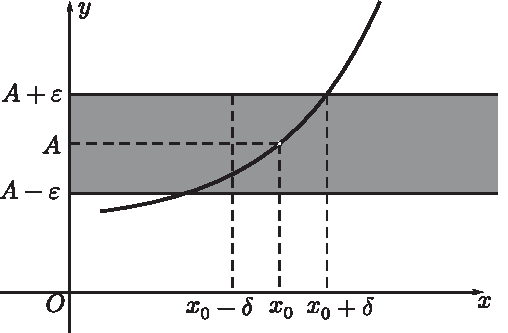
\includegraphics[scale=0.8]{pictures/C-1/极限1.pdf}
	\end{center}
	\sj \sj 
	\caption{极限的定义图解}
\end{figure}
\sj
\subsection{自变量趋于无穷大时函数的极限}
\tdefination[函数极限2]
设函数$f(x)$在当$|x|$大于某一正数时恒有定义.如果存在常数$A$,对于任意给定的正数$\varepsilon$(不论它多么小),总存在正数$X$使得当$x$满足不等式$|x|>X$时,对应的函数值$f(x)$都满足不等式
\begin{equation}
	|f(x)-A|<\varepsilon
\end{equation}
那么常数$A$就叫做函数$f(x)$当$x \to x_0$的\dy[极限]{JX},记作
\begin{equation}
	\lim\limits_{x\to \infty}f(x)=A \huo f(x)\to A(x \to \infty )
\end{equation}

\subsection{无穷小与无穷大}
\tdefination[无穷小]
如果函数$f(x)$当$x\to x_0\left(\mbox{或}x \to \infty  \right) $时的极限为$0$,那么称函数$f(x)$为当$x\to x_0\left(\mbox{或}x \to \infty  \right) $时的\dy[无穷小]{WQX}.记为
\begin{equation}
	\lim\limits_{x \to x_0}f(x)=0,\lim\limits_{x\to \infty}f(x)=0.
\end{equation}
特别地,以$0$为极限的数列${x_n}$称为$n\to \infty$时的\dy[无穷小]{WQX}.
\jg

\defination[无穷大]
设函数$f(x)$在$x_0$的某一去心邻域内有定义(或$|x|$趋于某一正数时有定义).如果对于任意给定的正数$M$(不论它多么大),总存在正数$\delta$(或正数$X$),只要$x$适合不等式$0<|x-x_0|<\delta$(或$|x|>X$),对应函数值$f(x)$总满足不等式
\begin{equation*}
	|f(x)|>M
\end{equation*}
那么称函数$f(x)$为当$x\to x_0\left(\mbox{或}x \to \infty  \right) $时的\dy[无穷大]{WQD}.记为
\begin{equation}
	\lim\limits_{x \to x_0}f(x)=\infty,\lim\limits_{x\to \infty}f(x)=\infty.
\end{equation}

\subsection{单侧极限}
\tdefination[左极限]
在 $\lim\limits_{x \to x_0}f(x)=A$的定义中,把$0<|x-x_0 |<\delta$改为$x_0-\delta <x<x_0$ ,那么$A$就叫做函数$f(x)$当$x \to x_0$时的\dy[左极限]{ZJX}.记作
\begin{equation}
	\lim\limits_{x \to x_0^-}f(x)=A \huo f(x_0^-)=A \huo \lim\limits_{x \to x_0 - 0}f(x)=A
\end{equation}

\defination[右极限]
在 $\lim\limits_{x \to x_0}f(x)=A$的定义中,把$0<|x-x_0 |<\delta$改为$x_0 <x<x_0+\delta$ ,那么$A$就叫做函数$f(x)$当$x \to x_0$时的\dy[右极限]{YJX}.记作
\begin{equation}
	\lim\limits_{x \to x_0^+}f(x)=A \huo f(x_0^+)=A \huo \lim\limits_{x \to x_0 + 0}f(x)=A
\end{equation}

\subsection{利用定义求函数的极限的解题方法}
\texample[可以直接求得$\delta$与$\varepsilon$的关系]
任意一个$\varepsilon$满足$|f(x)-A|<\varepsilon$,都能找到一个正数$\delta$使$0 < |x - x_0| < \delta$或$|x| > \delta$ ,这就说明了$\varepsilon$与$\delta $有个对应关系,即
\begin{equation}
	\delta=\varphi(\varepsilon)
\end{equation}
\par $\delta=\varphi(\varepsilon)$这个关于$\varepsilon$的函数可以是任意的.所以我们利用极限的定义来证明某个函数的极限时,只需找到$\varepsilon$和$\delta$之间的对应关系.这时,我们可以先利用$|f(x)-A|<\varepsilon$这个条件,然后构造出 $|x - x_0| < \varphi(\varepsilon)$的形式即可.(对于求数列的极限时$\delta$换成$N$即可.)

\examples 证明下列极限\\[0.5em]
\hspace*{0.8em} $1.\,\,\lim\limits_{x \to 3}2x-1=5$

\proof  设$\exists \delta,\forall \varepsilon$,当$0<|x-3|<\delta $时,$|2x-1-5|=|2x-6|=2|x-3|<\varepsilon$\quad \quad 【构造$|x-x_0 | < \varphi (\varepsilon)$】\\[0.5em]
即$\displaystyle |x-3|<\frac{\varepsilon}{2}$,故取$\displaystyle \delta = \frac{\varepsilon}{2}$时成立,证毕.\\[1.5em]
\hspace*{0.8em} $2.\,\,\displaystyle \lim\limits_{x \to \infty }\frac{1}{x}=0$\\[1em]
\proof  设$\exists N,\forall \varepsilon$,当$|x|>N$时,$\displaystyle \left| \frac{1}{x}-0\right| =\left| \frac{1}{x}\right|<\varepsilon$\hspace{13em}【构造$|x-x_0 | < \varphi (\varepsilon)$】\\[0.5em]
即$\displaystyle |x|>\frac{1}{\varepsilon}$,故取$\displaystyle N = \frac{1}{\varepsilon}$时成立,证毕.\\

\example[不能直接求得$\delta$与$\varepsilon$的关系]
\noindent 【方法一】放缩法\vspace{0.3em}
\par 这个时候我们可以将$|f (x) - A|$进行适当的放大,使得$\delta $与$\varepsilon$的关系容易求得,一般的放缩方法有:\\[0.5em]
\noindent (1) 将分母恒大于零的部分(可以含$x$)删去;\\[0.5em]
\noindent (2) 将分子恒小于零的部分删去(可以含$x$);\\[0.5em]
\noindent (3) 将幂函数的底数部分进行放缩.

\examples 证明$\displaystyle \lim\limits_{x \to 1}\sqrt{3x+1}=2.$

\proof 设$\exists \delta,\forall \varepsilon$,当$0<|x-1|<\delta $时,$\displaystyle |\sqrt{3x+1}-2|=\frac{3(x-1)}{\sqrt{3x+1}+2}\le \frac{3}{2}|x-1|<\varepsilon$\hspace{4em}【放缩构造】\\[0.5em]
即$\displaystyle |x-1|<\frac{2}{3}\varepsilon$,又$\displaystyle \sqrt{3x+1}$定义域为$\displaystyle x>-\frac{1}{3}$,那么$\displaystyle x-1>-\frac{4}{3}$,在一定范围内有$\displaystyle |x-1|<\frac{4}{3}$\hspace{1em}【判断定义域】\\[0.5em]
故取$\displaystyle \delta = \min \left\lbrace  \frac{2}{3}\varepsilon,\frac{4}{3} \right\rbrace $时成立,证毕.\hspace{27em}【取最小值】\\

\noindent 【方法二】先设后求再取值法\vspace{0.8em}
\par 放缩不是唯一的方法,我们还可以先设后求再取$\delta $最小值.\\[0.3em]
\noindent (1) 先化简式子,且含$|x-a|$项,这个时候可以用该方法;\\[0.5em]
\noindent (2) 设$\delta $的值为$f(a)$ (可以含$a,x$,也可以是常数);\\[0.5em]
\noindent (3) 解出$x$的范围,对非$|x - a|$的项进行放缩,将式子放大,同时使得非$|x - a|$的项转换为常量;\\[0.5em]
\noindent (4) 反解出$\delta = \varphi (\varepsilon)$;\\[0.5em]
\noindent (5) 取$\delta = \min \lbrace f(a),\varphi(\varepsilon)\rbrace$.\vspace{0.5em}
\par 当然通常放缩法和先设后求再取值法会结合用,这样就可以解决大部分题目.
\par 但是在后面的证明过程中,一般简单的函数极限可以直接用,所以一般情况下不会用定义证明极限.

\examples 证明$\lim\limits_{x \to a}x^2=a^2$

\proof 由于$|x^2-a^2|=|(x-a)(x+a)|=|x-a|\cdot |x+a| $,\hspace{16em}【找到$|x-a|$项】\\[0.5em]
设$\displaystyle |x-a|<\frac{1}{2}$,则$\displaystyle |x+a|=|x-a+2a|\le |x-a|+|2a|<\frac{1}{2}+|2a|.$ \hspace*{2em}【赋值$|x-a|$项,并放缩得出未知项的范围】\\[0.5em]
所以,设$\exists \delta,\forall \varepsilon$,当$0<|x-1|<\delta $时,$\displaystyle |x^2-a^2|=|x-a|\cdot |x+a|<\left( \frac{1}{2}+|2a|\right)|x-a|<\varepsilon $,\\[0.5em]
即$\displaystyle|x-a|<\frac{\varepsilon}{\frac{1}{2}+2|a|}$.\hspace{29em}【反解出$|x-a|$的范围】\\[0.5em]
故取$\displaystyle \delta = \min \left\lbrace  \frac{\varepsilon}{\frac{1}{2}+2|a|},\frac{1}{2} \right\rbrace $时成立,证毕.\hspace{26em}【取最小值】

\subsection{证明函数的极限不存在的方法}
\ttheorem[序列极限]
设函数$f (x)$在$a$点的一个空心邻域内有定义,并且$\lim\limits_{x \to a}f(x)=l$.假若是一串在该空心邻域内取值的序列,且
\begin{equation*}
	\lim\limits_{n \to \infty}x_n=a
\end{equation*}
则有
\begin{equation}
	\lim\limits_{n \to \infty}f(x_n)=l
\end{equation}
\par 这个定理为我们提供了一种\textbf{证明函数极限不存在的办法}:对于一个定义在$a$点的某空心邻域内的函数$f(x)$,如果能找到两串序列$\lbrace x'_n \rbrace $与$\lbrace x''_n\rbrace$它们都在$a$的该空心邻域内取值,且当$n\to \infty $时都以$a$为极限,而极限$\lim\limits_{n \to \infty }x'_n$与 $\lim\limits_{n \to \infty }x''_n$都存在但不相等,则$f(x)$在$x \to a$时不可能有极限.\jg

\example[证明函数的极限不存在]
\sj \examples 证明:函数$\displaystyle \sin \frac{1}{x}$在$x\to 0$时没有极限.

\proof 取$\displaystyle x'_n=\frac{1}{2n\pi }$,则$\displaystyle \sin \frac{1}{x'_n}=0$;而取$\displaystyle x''_n=\frac{1}{2n\pi+\frac{\pi}{2} }$,则$\displaystyle \sin \frac{1}{x'_n}=1.$\\[0.5em]
这时由于$n \to \infty \Rightarrow x'_n\to 0,x''_n \to 0, $且
\begin{equation*}
	\lim\limits_{n \to \infty} \sin \frac{1}{x'_n} \ne \lim\limits_{n \to \infty} \sin \frac{1}{x''_n} 
\end{equation*}
因此,函数$\displaystyle \sin \frac{1}{x}$在$x\to 0$时没有极限.

\section{利用极限运算法则和两个准则求极限}
\subsection{极限运算法则}
\ttheorem[极限运算法则1]
两个无穷小的和是无穷小.

\tl 有限个无穷小的和是无穷小.
\newpage
\theorem[极限运算法则2]
有界函数与无穷小的乘积是无穷小.

\tl 常数与无穷小的乘积是无穷小.

\tl 有限个无穷小的乘积是无穷小.\jg

\theorem[极限运算法则3]
如果$\lim f(x) = A, \lim g(x) = B$(这些函数都必须存在极限),那么
\begin{equation}
	\lim [f(x)\pm g(x)]=\lim f(x)\pm \lim g(x)=A \pm B
\end{equation}
\begin{equation}
	\lim[f(x)\cdot g(x)]=\lim f(x)\cdot \lim g(x)=A\cdot B
\end{equation}
若$B\ne 0$,那么
\begin{equation}
	\lim \left[ \frac{f(x)}{g(x)}\right] =\frac{\lim f(x)}{\lim g(x)}=\frac{A}{B}
\end{equation}

\tl 如果$\lim f(x)$存在,而$c$为常数,那么
\begin{equation}
	\lim [cf(x)]=c \lim f(x)
\end{equation}

\tl 如果$\lim f(x)$存在而$n$为正整数,那么
\begin{equation}
	\lim [f(x)]^n=[\lim f(x)]^n
\end{equation}

\theorem[极限运算法则4]
如果$\varphi(x) \ge \psi(x),$而$\lim \varphi(x)=A,\lim \psi(x)=B,$则$A \ge B.$\jg

\subsection{极限运算准则}
\ttheorem[单调有界数列极限一定存在]
(1)  \quad 若$x_{n+1} \le x_n(n\mbox{为正整数})$,且$x_n \ge m,$则$\lim\limits_{n \to \infty }x_n = A $存在,且$A \ge m$;
\par (2)  \quad 若$x_{n+1} \ge x_n(n\mbox{为正整数})$,且$x_n \le M,$则$\lim\limits_{n \to \infty }x_n = A $存在,且$A \le M$.

\theorem[夹逼定理]
设$g(x) \le f(x) \le h(x)$,若$\lim\limits_{x \to m}g(x)=A,\lim\limits_{x \to m}=A,(-\infty \le m \le +\infty)$则$\lim\limits_{x \to m}f(x)=A.$\jg

\subsection{例题}
\texample[利用极限运算法则和两个准则求极限]\sj
\examples 证明:$\lim\limits_{n \to \infty}q^n=0.(|q|<1)$

\proof 设$\displaystyle |q|=\frac{1}{1+a},a>0,$则$\displaystyle 0< q^n=\frac{1}{(1+a)^n}=\frac{1}{C^0_na^0=C^1_na^1+C^2_na^2+\cdots+C^n_na^n}<\frac{1}{C^1_na^1}=\frac{1}{na}.$\\[0.5em]
又$\displaystyle \lim\limits_{n \to \infty}\frac{1}{na}=0,\lim\limits_{n\to \infty}0=0,$由夹逼定理可得
\begin{equation*}
	\lim\limits_{n\to \infty}0 \le \lim\limits_{n \to \infty}q^n \le \lim\limits_{n \to \infty}\frac{1}{na}
\end{equation*}
故$\lim\limits_{n \to \infty}q^n=0.$\jg

\examples 证明:$\displaystyle a_n=\frac{a^n}{n!}(a\mbox{是大于1的任意常数})$存在极限.

\proof 当$n>[a]+1$时,有
\begin{equation*}
	0\le a_n =\frac{a^{[a]}}{[a]!}\cdot \frac{a}{[a]+1}\cdot \frac{a}{[a]+2}\cdot \,\,\cdots \,\,\cdot \frac{a}{n}<\frac{a^{[a]}}{[a]!}\cdot \frac{a}{n}
\end{equation*}
注意到$\displaystyle \frac{a^{[a]}}{[a]!}$是一个常数,所以$\displaystyle \lim\limits_{n \to \infty}\frac{a^{[a]}}{[a]!}\cdot \frac{a}{n}=0,$由夹逼定理可得
\begin{equation*}
	\lim\limits_{n \to \infty}a_n=0.
\end{equation*}

\examples 设常数$a>1,$对于任意自然数$k$,证明:
\begin{equation*}
	\lim\limits_{n \to \infty}\frac{n^k}{a^n}=0.
\end{equation*}
\hspace*{-0.5em}\proof 令$t=a-1$,则$t>0$,那么
\[
a_n=(1+t)^n=1+nt+\frac{n(n-1)}{2!}t^2+\cdots+\frac{n(n-1)\cdot(n-k)}{(k+1)!}t^{k+1}+\cdots+t^n,
\]
因此,当$n>1$时,$\displaystyle a^n>\frac{n(n-1)\cdots(n-k)}{(k+1)!}t^{k+1}$,于是
\[
0 \le \frac{n^k}{a^n}\le \frac{n^k}{\displaystyle \frac{n(n-1)\cdots(n-k)}{(k+1)!}t^{k+1}}=\frac{(k+1)!}{t^{k+1}}\cdot \frac{n^k}{n(n-1)\cdots(n-k)}=\frac{(k+1)!}{t^{k+1}}\cdot\frac{n^k}{\lambda_{k+1}n^{k+1}+\lambda_kn^k+\cdots+\lambda_1n+\lambda_0}
\]
其中$\lambda_0,\lambda_1,\cdots,\lambda_{k+1}$均为非零常数.注意到$\displaystyle \frac{(k+1)!}{t^{k+1}}$为常数,则
\begin{equation*}
	\begin{split}
		&\quad \, \lim\limits_{n \to \infty}\frac{(k+1)!}{t^{k+1}}\cdot\frac{n^k}{\lambda_{k+1}n^{k+1}+\lambda_kn^k+\cdots+\lambda_1n+\lambda_0}\\
		&=\lim\limits_{n \to \infty}\frac{(k+1)!}{t^{k+1}}\cdot\frac{1}{n}\cdot \frac{n^k}{\lambda_{k+1}+\lambda_kn^{-1}+\cdots+\lambda_1n^{-k}+\lambda_0n^{-k-1}}=0
	\end{split}
\end{equation*}
因此,由夹逼定理可得
\begin{equation*}
	\lim\limits_{n \to \infty}\frac{n^k}{a^n}=0.
\end{equation*}

\section{利用等价无穷小求极限}
\subsection{无穷小的分类}
\tdefination[无穷小的分类]
设$\alpha,\beta $是同一变化过程中的无穷小,$\displaystyle \lim \frac{\beta}{\alpha}$是这一过程的极限,$c$为常数,那么\\[0.5em]
\noindent (1) \quad $\displaystyle \lim \frac{\beta }{\alpha}=0$,则称$\beta $是$\alpha $的\dy[高阶无穷小]{GJWQX},记作$\beta = o(\alpha)$.\\[0.5em]
\noindent (2) \quad  $\displaystyle \lim \frac{\beta }{\alpha}=\infty$,则称$\beta $是$\alpha $的\dy[低阶无穷小]{DJWQX1}.\\[0.5em]
\noindent (3) \quad  $\displaystyle \lim \frac{\beta }{\alpha}=c \ne 0$,则称$\beta $是$\alpha $的\dy[同阶无穷小]{TJWQX}.\\[0.5em]
\noindent (4) \quad  $\displaystyle \lim \frac{\beta }{\alpha}=1$,则称$\beta $是$\alpha $的\dy[等价无穷小]{DJWQX2},记作$\beta \sim \alpha$.\\[0.5em]
\noindent (3) \quad  $\displaystyle \lim \frac{\beta }{\alpha^k}=c \ne 0$,则称$\beta $是$\alpha $的\dy[$k$阶无穷小]{KJWQX}.

\warn[
{\large \bf 0与``0"的区别}\vspace*{0.5em}\\
\hspace*{1em}(1)\quad ``0"指的是无穷小,设$\alpha$是某一变化过程中的无穷小,也就是说$x$趋于某一值时,极限为0.\vspace*{0.5em}\\
\hspace*{1em}(2)\quad 当0指的是实数0时,$\lim 0 \cdot f(x)=0$,这与$f(x)$无关,即使$\lim f(x)=\infty$,其结果仍然是0,因为0在这里是实数,而不是无穷小.
]


\subsection{常见的等价无穷小}
\ttheorem[常见的等价无穷小]
以下等价无穷小均为$x \to 0$这一变化过程,其中$x$也可替换为一个函数,即$f(x) \to 0$的情况也适用.
\begin{equation}
	\tan x \sim \sin x \sim x \sim \arcsin x \sim \arctan x
\end{equation}
\begin{equation}
	\ln (1+x) \sim x
\end{equation}
\begin{equation}
	x \sim \e^x -1
\end{equation}
\begin{equation}
	1-\cos x \sim \frac{x^2}{2}
\end{equation}
\begin{equation}
	\sec x -1 =\frac{1}{\cos x}-1 \sim \frac{x^2}{2}
\end{equation}
\begin{equation}
	(1+x)^a-1 \sim 1-ax
\end{equation}
\begin{equation}
	a^x-1 \sim \ln a \cdot x \,(a>0,a \ne 1)
\end{equation}
\subsection{等价无穷小求极限的本质}
等价无穷小求极限本质上是极限与1的相乘,而有等价无穷小的定义,1可以换成极限$\displaystyle 1=\lim\limits_{x \to x_0}\frac{\alpha }{\beta}$,再运用极限乘法运算法则计算即可.

\example[等价无穷小的误用]\sj
\examples \label{例 1.8}求极限$\displaystyle \lim\limits_{x \to 0}\frac{\tan x -\sin x}{\sin^3 x}$.

\errsolve  由于$\tan \sim \sin x \sim x$得$\displaystyle \lim\limits_{x \to 0}\frac{\tan x -\sin x}{\sin^3 x}=\lim\limits_{x \to 0}\frac{x-x}{\sin^3 x}=\lim\limits_{x \to 0}0=0.$

\errreason  在运用等价无穷小的时候没有考虑极限运算法则成立的条件.

\solvereason $\displaystyle \lim\limits_{x \to 0}\frac{\tan x -\sin x}{\sin^3 x}=\lim\limits_{x \to 0}\frac{\tan x}{\sin^3 x} - \lim\limits_{x \to 0}\frac{\sin x}{\sin^3 x}$实际上运用了法则$\lim [f(x)-g(x)]=\lim f(x)-\lim g(x),$\\[1em]即完整的错解解题步骤应为
\begin{equation*}
	\lim\limits_{x \to 0}\frac{\tan x -\sin x}{\sin^3 x}=\lim\limits_{x \to 0}\frac{\tan x}{\sin^3 x} - \lim\limits_{x \to 0}\frac{\sin x}{\sin^3 x}
	=\lim\limits_{x \to 0}\frac{\tan x}{\sin^3 x}\cdot \lim\limits_{x \to 0} \frac{x}{\tan x}-\lim\limits_{x \to 0}\frac{x}{\sin^3 x}
\end{equation*}
而极限运算法则成立的条件是$\lim f(x),\lim g(x)$存在,而$\displaystyle \lim\limits_{x \to 0}\frac{\tan x}{\sin^3 x}$不存在,因此解题错误.

\solve $\displaystyle \lim\limits_{x \to 0}\frac{\tan x -\sin x}{\sin^3 x}=\lim\limits_{x \to 0}\frac{\sin x(\sec x-1)}{\sin^3 x}=\lim\limits_{x \to 0}\frac{\sec x-1}{\sin^2 x} \cdot \lim\limits_{x \to 0}\frac{\frac{x^2}{2}}{\sec x -1} \cdot \lim\limits_{x \to 0}\frac{\sin x^2}{x^2}
=\frac{\frac{x^2}{2}}{x^2}=\frac{1}{2}.$\jg

\examples 求极限$\displaystyle \lim_{x \to 0} \frac{\sin \left(x^2 \sin{\frac{1}{x}}\right) }{x}.$

\errsolve $\displaystyle \lim_{x \to 0}\frac{\sin \left(x^2 \sin{\frac{1}{x}}\right) }{x}=\lim_{x \to 0}\frac{x^2 \sin \frac{1}{x}}{x}=\lim_{x \to 0}x\sin\frac{1}{x}=0.$

\errreason 对极限概念的理解不清晰,不仔细,没有严格判断等价无穷小的定义式是否满足极限的定义.

\solvereason 实际上,该错误解答的完整版本应该为:
\[
\lim_{x \to 0} \frac{\sin \left(x^2 \sin{\frac{1}{x}}\right) }{x}=\lim_{x \to 0} \frac{\sin \left(x^2 \sin{\frac{1}{x}}\right) }{x}\cdot\frac{x^2\sin \frac{1}{x}}{\sin \left( x^2 \sin \frac{1}{x}\right) }=\lim_{x \to 0}\frac{x^2\sin\frac{1}{x}}{x}=\lim_{x \to 0}x\sin \frac{1}{x}=0.
\]
但是极限
\[
\lim_{x \to 0}\frac{x^2\sin \frac{1}{x}}{\sin \left( x^2\sin \frac{1}{x}\right) }
\]
中,若$\displaystyle \sin \frac{1}{x}$取0,则这个极限式无意义(分母为0).故$\displaystyle x \ne \frac{1}{k \pi}(k \in Z).$\hspace*{11.5em}【判断定义域】\\[0.5em]
\hspace*{2em}这样的话,在点$x = 0$的任何一个去心邻域中都有无穷多个点没有定义,所以不存在一个去心邻域满足该极限式,
故极限不存在.\hspace*{24em}【判断是否能找到满足的去心邻域】\\[0.5em]
这里再次强调一下0与``0"的区别: 分母为0的时候并不是指无穷小量,而是真正意义上的0.

\solve 设$\exists \delta, \forall \varepsilon,$使得当$|x-0|<\delta$时,$\displaystyle \left| \frac{\sin \left( x^2\sin\frac{1}{x}\right) }{x}-0\right|<\varepsilon$,\\[0.5em]
由不等式$|\sin x|\le |x|$,得
\[
\left| \frac{\sin \left( x^2\sin\frac{1}{x}\right) }{x}\right| \le \left| \frac{ \left( x^2\sin\frac{1}{x}\right) }{x}\right| =\left| x \sin \frac{1}{x} \right|.
\]
由$\displaystyle \left| \sin \frac{1}{x} \right| \le 1$,得
\[
\left| \frac{\sin \left( x^2\sin\frac{1}{x}\right) }{x}\right| \le \left| \frac{ \left( x^2\sin\frac{1}{x}\right) }{x}\right| =\left| x \sin \frac{1}{x} \right|.\le |x|<\varepsilon
\]

\subsection{例题}
\sj
\example[等价无穷小的运用]
在下面的例题中,为了方便,省略了含有等价无穷小本质的式子.但是建议读者在实际做题的过程中还是要写完整,方便利用定义检查式子的合理性.
\examples 求极限$\displaystyle \lim_{x \to \infty}\left(\cos \frac{3}{x} \right)^{x^2} $

\solve 令$\displaystyle t=\frac{1}{x}$,则$x=\frac{1}{t},x\to \infty ,t \to 0.$
\[
\lim_{x \to \infty}\left(\cos \frac{3}{x} \right)^{x^2} =\lim_{t \to 0}(\cos 3t)^{\frac{1}{t^2}}=\lim_{t \to 0}\left[\left( 1-2\sin^2\frac{3t}{2}\right)^{\frac{1}{2\sin^2\frac{3t}{2}}} \right]^{\frac{2\sin^2\frac{3t}{2}}{t^2}} =\e^{\displaystyle -\lim_{t \to 0}\frac{2\sin^2\frac{3t}{2}}{t^2}}
\]
因为$\displaystyle \lim_{t \to 0}\frac{2\left( \displaystyle \frac{3t}{2}\right)^2 }{t^2}=\frac{9}{2},\,\therefore \lim_{x \to \infty }\left(\cos \frac{3}{x} \right)^{x^2}=\e^{ \displaystyle  -\lim_{t \to 0}\frac{2\sin^2\frac{3t}{2}}{t^2}}=\e ^{-\frac{9}{2}} $

\solveother 令$\displaystyle t=\frac{1}{x}$,则$\displaystyle x=\frac{1}{t},x\to \infty ,t \to 0.$
\[
\lim_{x \to \infty}\left( \cos \frac{3}{x}\right)^{x^2} =\lim_{t \to 0}(\cos 3t)^{\frac{1}{t^2}}=\e^{\lim\limits_{t \to 0}\ln(\cos 3t)^{\frac{1}{t^2}}}
\]
\[
\because \lim\limits_{t \to 0}\frac{1}{t^2}\ln(\cos 3t)=\lim\limits_{t \to 0}\frac{1}{t^2}\ln (\cos 3t)=\lim\limits_{t \to 0}\frac{1}{t^2}\ln \left[1+\left(-2\sin^2\frac{3t}{2}\right)\right]=\lim_{t \to 0}\frac{-2\sin^2\frac{3t}{2}}{t^2}=\lim\limits_{t \to 0}\frac{-2\left(\frac{3t}{2}\right)^2}{t^2}=-\frac{9}{2}.
\]
\[
\therefore \lim_{x \to \infty}\left( \cos \frac{3}{x}\right)^{x^2}=\lim\limits_{t \to 0}(\cos 3t)^{\frac{1}{t^2}}=\e^{\lim\limits_{t \to 0}\ln(\cos 3t)^{\frac{1}{t^2}}}=\e^{-\frac{9}{2}}.
\]

\inference[等价无穷小类型\uppercase\expandafter{\romannumeral1}]
以上是利用两种等价无穷小的解法,下面对这两种等价无穷小的用法归类.(这两个极限选一个用即可).若一个极限表达式有下列的形式(或者经过换元、取对数等方法变成这种形式),则很有可能用到这两种极限.
\begin{equation}
	\lim f(x)^{g(x)}
\end{equation}
其中$\lim f(x)=1,\lim g(x)$存在.

解法一\qquad 变形为:
\begin{equation}
	\lim\big[1+\big(f(x)-1\big)\big]^{g(x)}=\lim\big[1+\big(f(x)-1\big)\big]^{\frac{g(x)[f(x)-1]}{f(x)-1}}=\e^{\lim g(x)\cdot [f(x)-1]}
\end{equation}
而此时$\lim g(x) \cdot [f(x)-1]$是容易求得的.


解法二\qquad 变形为:
\begin{equation}
	\lim\big[1+\big(f(x)-1\big)\big]^{g(x)}=\e^{\lim \ln[1+\left( f(x)-1\right) ]}=\e^{\lim g(x)\cdot [f(x)-1]}
\end{equation}
而此时$\lim g(x) \cdot [f(x)-1]$也是容易求得的.

\examples 已知函数$f(x)$满足$\displaystyle \lim_{x \to 0}\frac{\sqrt{1+f(x)\sin 2x}-1}{\e^{3x}-1}=2$,求$\displaystyle \lim_{x \to 0}f(x).$

\solve $\displaystyle \lim_{x \to 0}\frac{\sqrt{1+f(x)\sin 2x}-1}{\e^{3x}-1}=\lim\limits_{x \to 0}\frac{1/2f(x)\sin 2x}{3x}=\lim_{x \to 0}\frac{1/2f(x)2x}{3x}=\frac{1}{3}\lim_{x\to 0}f(x)=2.$
\[
\therefore \lim_{x \to 0}f(x)=6.
\]

下面给出一个较难看出错误的例题.

\examples \label{例 1.12}求极限$\displaystyle \lim_{x \to 0}\left[ \frac{(1+x)^{\frac{1}{x}}}{\e}\right]^{\frac{1}{x}}.$

\errsolve $\displaystyle \lim_{x \to 0}\left[ \frac{(1+x)^{\frac{1}{x}}}{\e}\right]^{\frac{1}{x}}=\lim_{x \to 0}\left[ \frac{\e}{\e}\right]^{\frac{1}{x}}=1.$

\errreason 在运用等价无穷小的时候没有考虑极限运算法则成立的条件.

\solvereason $\displaystyle \lim_{x \to 0}\left[ \frac{(1+x)^{\frac{1}{x}}}{\e}\right]^{\frac{1}{x}}=\e^{\lim\limits_{x \to 0}\frac{1}{x}\ln\frac{(1+x)^{\frac{1}{x}}}{\e}},$
\[
\lim_{x \to 0}\frac{1}{x}\ln\frac{(1+x)^{\frac{1}{x}}}{\e}=\lim\limits_{x \to 0}\frac{1}{x}\left[ \ln(1+x)^{\frac{1}{x}} -\ln \e\right]=\lim\limits_{x \to 0}\frac{1}{x}\cdot\lim\limits_{x \to 0}\left[ \ln(1+x)^{\frac{1}{x}} -\ln \e\right]=\lim_{x \to 0}\frac{1}{x} \cdot \lim\limits_{x \to 0} \left[ \ln \e -\ln \e \right]=0.
\]
实际上,在$\displaystyle \lim\limits_{x \to 0}\frac{1}{x}\left[ \ln(1+x)^{\frac{1}{x}}-\ln \e \right]=\lim\limits_{x \to 0}\frac{1}{x}\cdot\lim\limits_{x \to 0}\left[ \ln(1+x)^{\frac{1}{x}} -\ln \e\right]$中用到了$\lim \big[f(x)\cdot g(x)\big]=\lim f(x) \cdot \lim  g(x)$,即用到了极限运算法则,而$\displaystyle \lim_{x \to 0}\frac{1}{x}$不存在,因此这种运算错误.

\solve $\displaystyle \lim_{x \to 0}\left[ \frac{(1+x)^{\frac{1}{x}}}{\e}\right]^{\frac{1}{x}}=\lim_{x \to 0}\left\lbrace1+\left[\frac{(1+x)^{\frac{1}{x}}}{\e}-1\right]\right\rbrace^{\frac 1x}=\lim_{x \to 0}\left\lbrace1+\left[\frac{(1+x)^{\frac{1}{x}}}{\e}-1\right]\right\rbrace^{ \frac{1}{(1+x)^{\frac 1x}-1}\cdot \frac{(1+x)^{\frac 1x}-1}{x}},$
\[
\because \lim\limits_{x \to 0}\left[\frac{(1+x)^{\frac{1}{x}}}{\e}-1\right]=0,\therefore \lim_{x \to 0}\left\lbrace1+\left[\frac{(1+x)^{\frac{1}{x}}}{\e}-1\right]\right\rbrace^{ \frac{1}{(1+x)^{\frac 1x}-1}\cdot \frac{(1+x)^{\frac 1x}-1}{x}}=\e^{\lim\limits_{x\to 0}\frac{(1+x)^\frac 1x-1}{x}},
\]
\[
\because \lim\limits_{x\to 0}\frac{\frac{(1+x)^\frac 1x}{\e}-1}{x}=\lim\limits_{x\to 0}\frac{(1+x)^\frac 1x-\e}{\e x}=\lim\limits_{x \to 0}\frac{\e^{\frac{1}{x}\ln(1+x)}-\e}{\e x}\xlongequal[]{\e^x-1 \sim x} \lim\limits_{x \to 0}\frac{\frac{1}{x}\ln(1+x)-1}{x}=\lim_{x \to 0}\frac{\ln (1+x)-x}{x^2}
\]
\[
\xlongequal[]{\ln(1+x)-x\sim-\frac{1}{2}x^2} \lim\limits_{x \to 0}\frac{-\frac{1}{2}x^2}{x^2}=-\frac{1}{2}
\]
\[
\therefore \lim_{x \to 0}\left[ \frac{(1+x)^{\frac{1}{x}}}{\e}\right]^{\frac{1}{x}}=\e^{\lim\limits_{x\to 0}\frac{(1+x)^\frac 1x-1}{x}}=\e^{-\frac{1}{2}}=\frac{\sqrt{\e}}{\e}.
\]

\inference[等价无穷小求极限]\sj
\begin{enumerate}
	\item 判断并构造等价无穷小的类型(7 种);
	\item 利用等价无穷小求极限的本质列出计算式;
	\item 判断等价无穷小的极限式中能否找到满足定义域的去心邻域使得极限存在:
	\begin{enumerate}[(i)]
		\item 若存在,则利用等价无穷小解题;
		\item 若不存在,则用其它方法求解(如利用函数定义、夹逼准则等).
	\end{enumerate}
	\item 检验计算的每一步是否都符合极限运算法则的前提条件.
\end{enumerate}
\vspace*{-2em}
\warn[
\hspace*{2em}1. 以上等价无穷小都只在$x\to 0$的情况下才成立,$x$趋于其它值时不成立.\\
\hspace*{2em}2. 只有等价无穷小的定义式存在极限的前提下,即在函数$f (x)$的定义域内能找到一个完整的去心邻域,$x$才可以用任意函数$f(x)$替换.若等价无穷小的定义式都不存在极限,又谈何等价无穷小.\\
下面给出常见的一些不可以用等价无穷小替换的函数.\jg\\
\examples $\displaystyle x \to 0,\sin\left(x \sin \frac 1x\right) \not \sim x\sin \frac{1}{x},\sin\left(x\cos \frac 1x\right)\not \sim x \cos \frac 1x$\\
\hspace*{2em}3. 在运用等价无穷小计算极限的时候要特别要注意在替换的过程中只有符合极限的运算法则,才可以进行
替换(通常极限的运算法则不明显,需要仔细计算),前面已经给出了两个详细的例子.
]

\section{函数连续性}
\subsection{函数连续性的定义}
\tdefination[函数在某点的连续性\uppercase\expandafter{\romannumeral1}]
设函数$y=f(x)$在点$x_0$的某一邻域内有定义,如果
\begin{equation}
	\lim\limits_{\Delta x \to 0}\Delta y=\lim\limits_{\Delta x \to 0}\big[f(x_0+\Delta x)-f(x_0)\big]=0.
\end{equation}
那么就称函数$y=f(x)$在点$x_0$处\dy[连续]{LX}.

\defination[函数在某点的连续性\uppercase\expandafter{\romannumeral2}]
设函数$y=f(x)$在点$x_0$的某一邻域内有定义,如果
\begin{equation}
	\lim\limits_{x \to x_0} f(x)=f(x_0).
\end{equation}
那么就称函数$y=f(x)$在点$x_0$处\dy[连续]{LX}.\jg

即$f(x)$在点$x_0$处连续$\Longleftrightarrow \forall \varepsilon>0,\exists \delta>0,$当$|x-x_0|<\delta$时,都有$|f(x)-f(x_0)|<\varepsilon$

\defination[左连续]
如果$\lim\limits_{x \to x_0^-}f(x)=f(x_0^-)$存在且等于$f(x_0)$,即$f(x_0^-)=f(x_0)$,那么就称函数$y=f(x)$在点$x_0$处\dy[左连续]{ZLX}.

\defination[右连续]
如果$\lim\limits_{x \to x_0^+}f(x)=f(x_0^+)$存在且等于$f(x_0)$,即$f(x_0^+)=f(x_0)$,那么就称函数$y=f(x)$在点$x_0$处\dy[右连续]{YLX}.

\warn[\hspace*{2em}函数在某点连续的充要条件是在该点的左极限和右极限都存在且都等于函数该点处的函数值.或者说函数在该点既左连续又右连续.(证明函数在某点处是否连续的方法)]


\defination[函数在某个区间的连续性]
在区间上每一点都连续的函数,叫做在该区间上的连续函数,或者说函数在该区间上连续.如果区间包括端点,那么函数在右端点是指右端点的左连续,在左端点是指左端点的右连续.

\blackbf[连续函数的图形是一条连续而不间断的线(可能是直线,也可能是曲线).]

\subsection{函数的间断点}
\tdefination[函数的间断点]
设函数$y=f(x)$在点$x_0$的某一邻域内有定义.在此前提条件下,如果函数有下列三种情况之一:\\[0.5em]
(1) 在$x=x_0$处没有定义;\hspace{12em}(2) 虽在$x=x_0$处有定义,但是$\displaystyle \lim\limits_{x \to x_0}f(x)$不存在;\\[0.5em]
(3) 虽在$x=x_0$处有定义,$\displaystyle \lim\limits_{x \to x_0}f(x)$存在,但$\displaystyle \lim_{x \to x_0}f(x) \ne f(x_0)$.\\[0.5em]
那么就称函数$f(x)$在点$x_0$处不连续,而点$x_0$称为函数$f(x)$的\dy[不连续点]{BLXD}或\dy[间断点]{JDD}.

如果$x_0$是函数$f(x)$的间断点,但左极限$f(x_0^-)$和右极限$f(x_0^+)$都存在,那么点$x_0$就称为函数$f(x)$的\dy[第一类间断点]{DYLJDD},不是第一类间断点的任何间断点都是\dy[第二类间断点]{DELJDD}.常见的具体分类见下表\ref{函数间断点的分类}.
\begin{table}[!htb]
	\centering
	\renewcommand{\arraystretch}{1}
	\setlength{\tabcolsep}{14mm}{
		\begin{tabular}{cc}
			\toprule[1.5pt] 
			第一类间断点 & 第二类间断点 \\
			\midrule
			可去间断点 & 无穷间断点\\
			跳跃间断点 & 震荡间断点\\
			\bottomrule[1.5pt]
		\end{tabular}  
	}
	\caption{函数间断点的分类}
	\renewcommand{\arraystretch}{1}
	\label{函数间断点的分类}
\end{table} 
\vspace*{-3em}

\defination[无穷间断点]
若$x_0$是函数$f(x)$的间断点,且$\lim\limits_{x \to x_0}f(x)=\infty $,那么我们称点$x_0$是函数的\dy[无穷间断点]{WQJDD}.\jg

\simpleexamples $\displaystyle x=\frac{\pi}{2}$是函数$y=\tan x$的无穷间断点.

\defination[振荡间断点]
若$x_0$是函数$f(x)$的间断点,且当$x \to x_0$时,函数值在多个值之间变动无穷多次,那么我们称点$x_0$是函数$f(x)$的\dy[振荡间断点]{ZDJDD}.\jg

\simpleexamples $\displaystyle x = 0$是函数$\displaystyle y =\sin\frac{1}{x}$的振荡间断点.
\warn[
\kg 若点$x_0$是函数$f(x)$的振荡间断点,那么在函数$f(x)$在点$x_0$处的任意的去心邻域都无确定的值.
进一步说,如果函数$f(x)$的导函数是$f'(x)$,点$x_0$是导函数$f'(x)$的振荡间断点,那么在$x_0$的任意去心邻域中函数$f(x)$的导数都不存在.
]
\vspace*{-1em}

\defination[可去间断点]
若点$x_0$是函数$f(x)$的间断点,且$f(x)$在点$x_0$处没有定义,而$\lim\limits_{x \to x_0}f(x)=f(x_0),$那么我们称点$x_0$是函数$f(x)$的\dy[可去间断点]{KQJDD}.\jg

\simpleexamples $\displaystyle x=1$是函数$\displaystyle y=\frac{x^2-1}{x-1}$的可去间断点.

\defination[跳跃间断点]
若点$x_0$是函数$f(x)$的间断点,且$f(x)$在点$x_0$处有定义,而$f(x_0^-)=f(x_0^+)$,那么我们称点$x_0$是函数$f(x)$的\dy[跳跃间断点]{TYJDD}.

\simpleexamples $\displaystyle x=0$是函数
$
\displaystyle
\begin{cases}
	x-1&,x<0\\
	0&,x=0\\
	x+1&,x>0
\end{cases}
$
的跳跃间断点.

\begin{tcolorbox}[sidebyside,colframe=red!75!black, colback=yellow!10!white,title=注意,sidebyside align=top seam,
	righthand width=4cm,fonttitle =\CJKfamily{heiti}]
	\kg 可去间断点的定义是左右极限相等即可,与函数在该点处是否有定义无关.关于这个很容易犯错,下面给出一个例子详细说明.
	\[
	f(x)=
	\begin{cases}
		x^2-1,&x<-3\\
		-1,&x=-3\\
		-3x-1,&-3<x\le 0
	\end{cases}
	\]
	如图,$\lim\limits_{x \to -3^-}f(x)=\lim\limits_{x \to -3^-}x^2-1=(-3)^2-1=8.$\\[0.5em]
	$\lim\limits_{x \to -3^+}=\lim\limits_{x \to -3^+}-3x-1=(-3)^2-1=8.$\\[0.5em]
	所以,$\lim\limits_{x \to -3^-}f(x)=\lim\limits_{x \to -3^+}f(x)=8 \neq f(-3).$\\[0.5em]
	即$x=-3$是函数$f(x)$的可去间断点.
	\tcblower
	\centering
	\vspace*{1cm}
	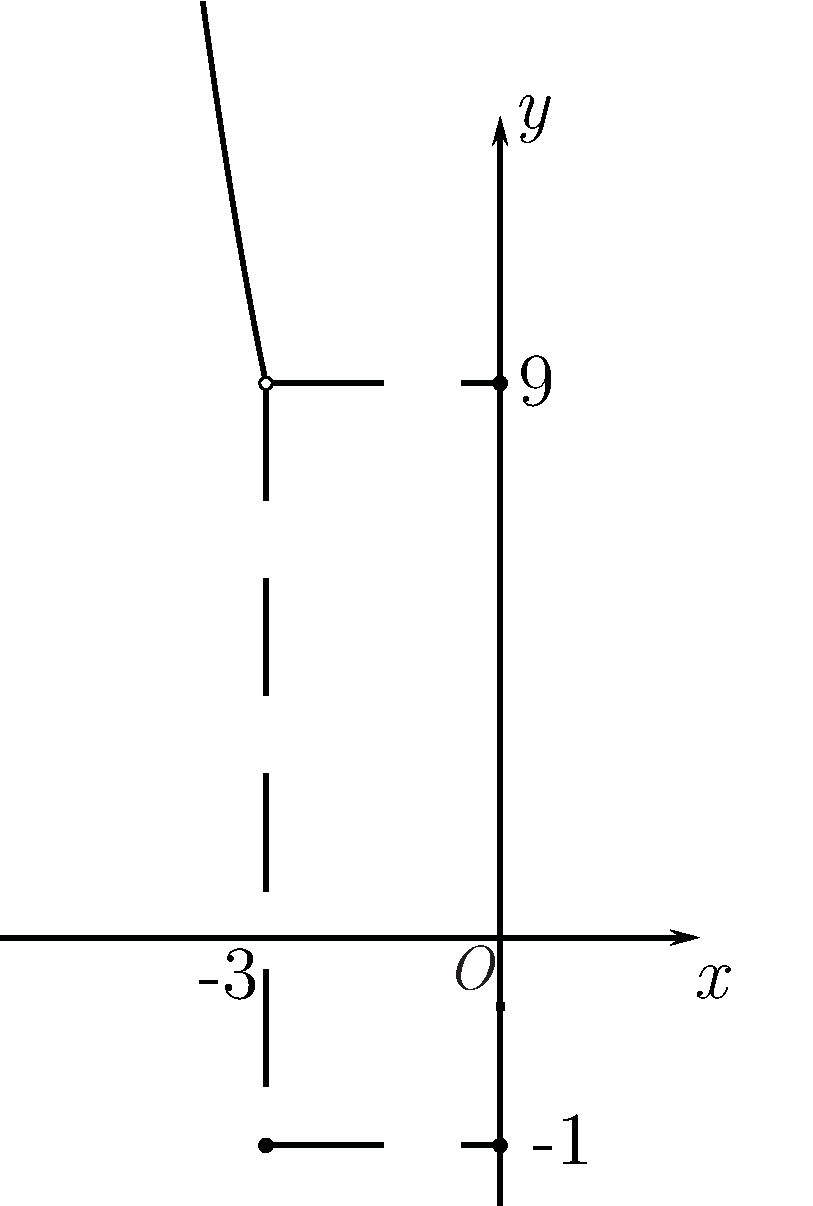
\includegraphics[width=\linewidth]{pictures/C-1/可去间断点.pdf}
\end{tcolorbox}

\inference[判断间断点的类型]
\begin{center}
	\begin{tikzpicture}[node distance=1.2cm]
		%定义流程图具体形状
		\node (A) [minimum height=0cm,draw, node distance=1cm,inner sep=8pt] {\quad 判断$x$处是否有左右极限\quad \quad };
		\node (A2) [minimum height=0cm,draw, below of=A,node distance=1.2cm,inner sep=8pt,xshift =9cm] {无穷间断点/振荡间断点};
		\node (B) [minimum height=0cm,draw, below of=A,node distance=2.4cm,inner sep=8pt] {\quad   判断左右极限是否相等 \quad \quad  };
		\node (B2) [minimum height=0cm,draw, below of=B,node distance=1.2cm,inner sep=8pt,xshift =8.05cm] {跳跃间断点};
		\node (C) [minimum height=0cm,draw, below of=B,node distance=2.4cm,inner sep=8pt] {\quad   判断$x$ 处的函数值 \quad \quad  };
		\node (C2) [minimum height=0cm,draw, below of=C,node distance=1.2cm,inner sep=8pt,xshift =8.45cm] {函数在$x$处连续};
		\node (D) [minimum height=0cm,draw, below of=C,node distance=2.4cm,inner sep=8pt] {\quad   可去间断点 \quad \quad  };
		
		
		%连接具体形状
		\draw[arrows={-Stealth[scale=0.8]}](A) -- (B) node[midway,left=0.5cm,above=-0.3cm]{有} ;
		\draw[arrows={-Stealth[scale=0.8]}](A) --+(0,-1.2cm) node[midway,right=3.5cm,above=-0.3cm]{没有}|-(A2) ;
		\draw[arrows={-Stealth[scale=0.8]}](B) -- (C) node[midway,left=0.5cm,above=-0.3cm]{相等} ;
		\draw[arrows={-Stealth[scale=0.8]}](B) --+(0,-1.2cm) node[midway,right=3.5cm,above=-0.3cm]{不相等}|-(B2) ;
		\draw[arrows={-Stealth[scale=0.8]}](C) -- (D)node[midway,left=1.3cm,above=-0.3cm]{函数值$=$极限} ;
		\draw[arrows={-Stealth[scale=0.8]}](C) --+(0,-1.2cm) node[midway,right=3.5cm,above=-0.3cm]{函数值$\neq$极限/无定义}|-(C2) ;
	\end{tikzpicture}
\end{center}

\subsection{连续函数的运算}
\ttheorem[连续函数的加减乘除]
设函数$f(x)$和$g(x)$在点$x_0$处连续,则它们的和(差)$f \pm g$、积$f \cot g$及商$\dfrac{f}{g}\,(g(x_0)\neq 0)$都在点$x_0$处连续.

\theorem[反函数的连续性]
如果函数$y=f(x)$在一个区间上连续且单调,那么它的反函数也在对应的区间连续且单调与原函数相同.


\theorem[复合函数的连续性\uppercase\expandafter{\romannumeral1}]
设函数$\lim\limits_{x \to x_0}g(x)=u_0$,,且函数$y=f(u)$在$u=u_0$处连续,则
\begin{equation}
	\lim\limits_{x \to x_0}f\big[g(x)\big]=\lim\limits_{u \to u_0}f(u)=f(u_0)
\end{equation}
\vspace*{-2em}

\warn
[
\kg $g(x)$可以不在点$x=x_0$处有连续,但是必须有极限.
]

\theorem[复合函数的连续性\uppercase\expandafter{\romannumeral2}]
设函数$u=g(x)$在$x=x_0$处连续,且$g(x_0)=u_0$,函数$y=f(x)$在$x=u_0$处连续,则复合函数$y=f\big[g(x)\big]$也在$x=x_0$处连续.\jg

\theorem[初等函数的连续性]
一切初等函数在其定义域内都是连续函数.\jg

\subsection{连续函数的性质}

\defination[最大值与最小值]
对于在区间$I$上有定义的函数$y=f(x)$,如果有$x_0 \in I$,使得任意一个$x$都有
\[
f(x)\le f(x_0)\quad\big(\,f(x) \geq f(x_0) \,\big)
\]
那么我们称$f(x_0)$是函数$y=f(x)$在区间$I$上的最大值(最小值).
\jg

\theorem[最大值最小值定理]
在闭区间上连续的函数在该区间上一定有界且一定能取到它的最大值和最小值.

\warn
[
\kg 如果函数在开区间内连续,或者在闭区间上有间断点,那么函数不一定有界且不一定能取到它的最大值或最小值.特别地,如果函数单调,且在开区间内连续,那么这个函数一定无界且无最大值和最小值.
]


\theorem[零点存在性定理]
设函数$f(x)$在闭区间$[a,b]$上连续,且$f(a)$与$f(b)$异号,即$f(a)\cdot f(b)<0$,则在开区间$(a,b)$内至少有一点$\xi$,使得
\[
f(\xi)=0
\]

\theorem[介值定理]
设函数$f(x)$在闭区间$[a,b]$上连续,且在这区间的取不同的函数值$f(a)=A,f(b)=B$,则对于$A$与$B$之间的任意一个数$C$,在开区间$(a,b)$内至少有一点$\xi$,使得
\[
f(\xi)=C(a<\xi<b)
\]

\tl 在闭区间$[a,b]$上连续的函数$f(x)$的值域为$[m,M]$,其中$m$与$M$依次为$f(x)$在$[a,b]$上的最小值与最大值.

\section{补充题型}
\subsection{求递归数列的极限}
\texample[求递归数列的极限]\sj
\examples 已知$x_1>0,x_{n+1}=\dfrac{1}{2}\left(x_n+\dfrac{a}{x_n}\right),(a>0,n=1,2,\ldots),$证明$\lim\limits_{n \to \infty} x_n$存在,并求该极限.

\solve $\displaystyle x_{n+1}=\frac 12\left(x_n+\frac{a}{x_n}\right)\ge \frac 12 \cdot 2\sqrt{x_n\cdot \frac{a}{x_n}}=\sqrt{a}$,所以$n>2$时,$x_n \ge \sqrt{a},$又
\[
x_{n+1}-x_n=\frac{1}{2}\left(\frac{a}{x_n}-x_n\right)\le\frac{1}{2}\left(\frac{a}{\sqrt{a}}-\sqrt{a}\right)=0
\]
所以数列$\{x_n\}$是单调递减数列,所以$\max x_n=\max\{x_1,x_2\}$,即$0<x_n<\max{x_1,x_2}$,即$\{x_n\}$是有界数列.
综上,数列$\{x_n\}$是单调有界数列,由极限存在法则知$\lim\limits_{n \to \infty}x_n$一定存在.设$\lim\limits_{n \to \infty}x_n=\lim\limits_{n \to \infty}x_{n+1}=c>0.$则$n \to \infty$时,有
\[
x_{n+1}=\frac{1}{2}\left(x_n+\frac{a}{x_n}\right)\,(n \to \infty) \quad \Rightarrow \quad c=\frac 12\left( c+\frac ac \right) \quad \Rightarrow \quad c^2=a \quad \Rightarrow \quad c=\sqrt{a}. 
\]
故$\lim\limits_{n \to \infty}x_n=\sqrt{a}.$

\examples 已知$x_1=1,x_{n+1}=\sqrt{2+x_n},\,(n=1,2,\ldots),$证明$\lim\limits_{n \to \infty }x_n$存在,并求该极限.

\solve 下面用数学归纳法证明$x_n<2$.
\begin{enumerate}[(i)]
	\item 当$n=1$时,$x_n=x_1=1<2$成立.
	\item 设$n=k$时,$x_n=x_k<2$成立.
	\item 当$n=k+1$时,$x_n=x_{k+1}=\sqrt{2+x_k}<\sqrt{2+2}=2,$也成立.
\end{enumerate}
所以$0<x_n<2.$故数列$\{x_n\}$是有界数列.又
\[
x_{n+1}-x_n=\sqrt{2+x_n}-x_n=\frac{2}{\sqrt{2+x_n}+x_n}>0.
\]
所以数列$\{x_n\}$是单调递增数列,又数列$\{x_n\}$有界,故数列$\{x_n\}$是单调有界数列,由极限存在法则可知$\lim\limits_{n \to \infty}x_n$一定存在.设$\lim\limits_{n \to \infty}x_n=\lim\limits_{n \to \infty}x_{n+1}=c>0.$则$n \to \infty$时,有
\[
x_{n+1}=\sqrt{2+x_n} \quad \Rightarrow \quad c=\sqrt{2+c} \quad \Rightarrow \quad c^2-c-2=0 \quad \Rightarrow \quad (c-2)(c+1)=0 \quad \Rightarrow \quad c=2.
\]
故$\lim\limits_{n \to \infty}x_n=2.$

\inference[求递归数列的极限]
\vspace*{1em} \noindent  \hspace*{0.2em}  \tcbox[colframe =ForestGreen
, colback =ForestGreen!15!white,boxrule=0.5mm,size=small,on line]{\color{ForestGreen}{{\CJKfamily{heiti}题目模板}}}\hspace{1.5em}
已知$x_1=a,x_{n+1}=f(x_n),$判断$\lim\limits_{n \to \infty }x_n$是否存在,若存在则求该极限.\jg\jg

\noindent \highlights[第一步 \quad 找答案]

做这类题,首先要做的就是先把答案猜出来,具体方法如下:
假设$\lim\limits_{n \to \infty}x_n$存在,且$x_n>0$,得到式子$\lim\limits_{n \to \infty}x_{n+1}=c>0$,即$c=f(c)$,求出$c$的值.($x_n<0$类似)
\begin{enumerate}[(i)]
	\item 若无解,则$\lim\limits_{n \to \infty}x_n$不存在;
	\item 若有解,注意判断解的合理性,通常只有一个解$c_0>0\big(x_n>0\big)$或$c_0<0\big(x_n<0\big)$,则$\lim\limits_{n \to \infty}x_n=c_0$.
\end{enumerate}
\jg

\noindent \highlights[第二步 \quad 证有界]

由上面的极限可以知道,
\begin{enumerate}[]
	\item 若数列$\{x_n\}$单调递增,则证$x_n \le c_0$;
	\item 若数列$\{x_n\}$单调递减,则证$\max \{x_1,x_2\} \ge x_n \ge c_0$.
\end{enumerate}
\sj
\warn
[
\kg 可以先不证明数列的单调性,但是要用赋值法先确定数列的单调性,就可以找到证明的方向,就可以容易用数学归纳法证明.
]
\jg

\noindent \highlights[第三步 \quad 证单调]

证单调直接用定义即可:\sj
\begin{multicols}{2}
	\noindent1.$\,\,x_{n+1}-x_n=f(x_n)-x_n$.
	\begin{enumerate}[(i)]
		\item $x_{n+1}-x_n>0\Rightarrow\{x_n\}$是单调递增数列;
		\item $x_{n+1}-x_n<0\Rightarrow\{x_n\}$是单调递减数列.
	\end{enumerate}
	2.$\,\,\dfrac{x_{n+1}}{x_n}=\dfrac{f(x_n)}{x_n}$.
	\begin{enumerate}[(i)]
		\item $x_{n+1}/x_n>1\Rightarrow \{x_n\}$是单调递增数列;
		\item $x_{n+1}/x_n<1\Rightarrow \{x_n\}$是单调递减数列;
	\end{enumerate}
\end{multicols}
\sj
\warn
[
\kg 在有变号的数列中第二种方法不适用.
]
\jg

\noindent \highlights[第四步 \quad 求极限]

由于$x_n$单调有界,由极限存在法则可知$\lim\limits_{x_n}$一定存在.$\lim\limits_{n \to \infty}x_n=\lim\limits_{n \to \infty}x_{n+1}=c>0,$即$c=f(c)$,求解这个方程后可以求出$c$的值,在步骤一中已经求出,可以直接写结果.
\warn
[
\kg $\lim\limits_{n \to \infty}x_n=\lim\limits_{n \to \infty}x_{n+1}=c$成立的前提条件是数列${x_n}$单调有界(或$\{x_n\}$收敛).
]

\subsection{极限存在求参数}
\texample[极限存在求参数]\sj

\examples 求实数$a,b$使得
\[
\lim\limits_{x \to 1}\frac{\sqrt{ax^2-2ax+b}-2}{x^2-2x+1}
\]
存在,并求出该极限.

\solve 由于$\lim\limits_{x \to 1}(x^2-2x+1)=0$.即分母为无穷小量.要使极限存在,则分子也为无穷小量,即
\[
\lim\limits_{x \to 1}\big[\sqrt{ax^2-2ax+b}-2\big]=0 \quad \Rightarrow \quad \sqrt{a-2a+b}-2=0 \quad \Rightarrow \quad \sqrt{b-a}=2 \quad \Rightarrow b-a=4.
\]
代入原极限式,并令$t=x-1,$,则$x=t+1,x\to1,t \to 0,$可得
\[
\begin{split}
	\lim\limits_{x \to 1}\frac{\sqrt{ax^2-2ax+b}-2}{x^2-2x+1}&=\lim\limits_{t \to 0}\frac{\sqrt{at^2+b-a}-2}{t^2}=\lim\limits_{t \to 0}\frac{\sqrt{at^2+4}-2}{t^2}\\
	&=\lim\limits_{t \to 0}\frac{at^2}{t^2\big(\sqrt{at^2+4}+2\big)}=\lim\limits_{t \to 0}\frac{a}{\sqrt{at^2+4}+2}=\frac{a}{4}.
\end{split}
\]
所以,当$b-a=4$时,均有
\[
\lim\limits_{x \to 1}\frac{\sqrt{ax^2-2ax+b}-2}{x^2-2x+1}=\frac a4.
\]

\examples 求实数$a,b$使得
\[
\lim\limits_{x \to 0}\frac{1+a\cos2x+b\cos4x}{x^4}
\]
存在,并求该极限.

\solve 
\[
\begin{split}
	\lim\limits_{x \to 0}\frac{1+a\cos2x+b\cos4x}{x^4}&=\lim\limits_{x \to 0}\frac{1+a\cos2x+b\cos4x}{x^4}\\
	&=\lim\limits_{x \to 0}\frac{1+a\cos 2x+b(2 \cos^22x-1)}{\big(\sin^2x\big)^2}\\
	&=\lim\limits_{x \to 0}\frac{1+a\cos 2x+2b \cos^22x-b}{\left(\frac{\cos 2x-1}{2}\right)^2}\\
	&=4\lim\limits_{x \to 0}\frac{2b\left(\cos^2 2x+\frac{a}{2b}\cos 2x +\left( \frac{a}{2b}\right)^2 -\frac{a^2}{16b^2}  \right)+1-b }{\left(\cos 2x-1\right)^2}\\
	&=4\lim\limits_{x \to 0}\frac{2b\left(\cos^2 2x+\frac{a}{2b}\cos 2x +\left( \frac{a}{2b}\right)^2 \right)+1-\frac{a^2}{8b} -b }{\left(\cos 2x-1\right)^2}\\
	&=4\lim\limits_{x \to 0}\frac{2b\left(\cos 2x +\frac{a}{4b}\right)^2+1-\frac{a^2}{8b} -b }{\left(\cos 2x-1\right)^2}\\
\end{split}
\]
要使极限存在,则要消去分母$\left(\cos 2x-1\right)^2$,比对系数得:
\[
\begin{cases}
	\dfrac{a}{4b}=-1\\[0.5em]
	1-\dfrac{a^2}{8b}-b=0
\end{cases}
\quad 
\Rightarrow
\quad 
\begin{cases}
	a=-\dfrac{4}{3}\\[0.5em]
	b=\dfrac{1}{3}
\end{cases}
\]
综上,当
$
\begin{cases}
	a=-\dfrac{4}{3}\\[0.5em]
	b=\dfrac{1}{3}
\end{cases}
$
时,极限
$
\lim\limits_{x \to 0}\dfrac{1+a\cos2x+b\cos4x}{x^4}
$
存在,且为$\dfrac{8}{3}.$

\subsection{分数型极限}

\texample[分数型极限]
关于这个题型先给出一个定理.

\theorem[分数型极限]
\begin{equation}
	\lim\limits_{x \to \infty}\frac{a_nx^n+a_{n-1}x^{n-1}+\cdots+a_2x^2+a_1x+a_0}{b_mx^m+b_{m-1}x^{m-1}+\cdots+b_2x^2+b_1x+b_0}=
	\begin{cases}
		0&,n<m\\
		\dfrac{a_n}{b_m}&,n=m\\
		\infty&,n>m
	\end{cases}
\end{equation}
\begin{equation}
	\lim\limits_{x \to 0}\frac{a_nx^n+a_{n-1}x^{n-1}+\cdots+a_2x^2+a_1x+a_0}{b_mx^m+b_{m-1}x^{m-1}+\cdots+b_2x^2+b_1x+b_0}=
	\begin{cases}
		\infty&,n<m\\
		\dfrac{a_n}{b_m}&,n=m\\
		0&,n>m
	\end{cases}
\end{equation}
\warn
[
\kg 这个定理只适合变量趋于0或$\infty$的情况.
]
通常这种类型还有几种变形,下面给出一个例子.

\examples 求极限$\lim\limits_{x \to +\infty}\dfrac{(x+1)(x^2+1)\cdot\,\cdots\,\cdot(x^n+1)}{\big[(nx)^n+1\big]^{\frac{n+1}{2}}}$.

\solve 由上面的定理可知,我们只需要考虑分子和分母的最高次项即可.\\[0.5em]
因为$(x+1)(x^2+1)\cdots(x^n+1)$的最高次项为$\displaystyle x^{\frac{n(n+1)}{2}}$,$\big[(nx)^n+1\big]^{\frac{n+1}{2}}$的最高次项为$\displaystyle (nx)^{\frac{n(n+1)}{2}}$.所以
\[
\lim\limits_{x \to +\infty}\dfrac{(x+1)(x^2+1)\cdot\,\cdots\,\cdot(x^n+1)}{\big[(nx)^n+1\big]^{\frac{n+1}{2}}}=\lim\limits_{x \to +\infty}\dfrac{x^{\frac{n(n+1)}{2}}}{(nx)^{\frac{n(n+1)}{2}}}=\frac{1}{n^{\frac{n(n+1)}{2}}}.
\]

\vspace*{-2em}
\summarize
[
\kg 其实看起来解题过程比较复杂,但是其实本质比较简单,弄清楚这种题型的做题方法如下:\\
1. 观察式子,判断题型是否为分数型;\\
2. 确定为分数型题型后,判断分数的分母和分子最高的次数的大小;\\
3. 运用定理运算极限即可.\\
\kg 特别注意的是,有些时候不是很好判断是否为分数型,像上面的例题.这个时候可以观察分子分母是否是高次多项式.如果分子和分母都是高次多项式,那么就可以尝试用分数型的解题方法来尝试解题.\\
\kg 可能还有的题需要换元以后才能得到这个分数型极限.
]

\subsection{已知一个极限式求另一极限式}
\examples 若$\displaystyle \lim\limits_{x \to 0}\left(\frac{f(x)-1}{x}-\frac{\sin x}{x^2}\right)=2$,求$\lim\limits_{x \to 0}f(x).$

\solve 记$\alpha = \dfrac{f(x)-1}{x}-\frac{\sin x}{x^2},$由题可知$\lim\limits_{x \to \alpha =0},$即
\[
f(x)=1+\alpha x+\frac{\sin x}{x}+2x \quad \Rightarrow \quad \lim\limits_{x \to 0}f(x)=\lim\limits_{x \to 0}\left( 1+ \alpha x +\frac{\sin x}{x} +2x\right) 
\]
由极限四则运算,得
\[
\lim\limits_{x \to 0}f(x)=\lim\limits_{x \to 0}\left( 1+ \alpha x +\frac{\sin x}{x} +2x\right) =1+0+1+0=2.
\]
\sj
\summarize
[
\kg 这是一类知道含$f(x)$的多项式的极限,求$\lim f(x)$的一类题,很巧妙地运用了换元法.
]

\subsection{求和式的极限}
\texample[求和式的极限]\sj
求和式的极限在高等数学教材中目前有两种可行的方法:定积分法和夹逼定理法.\jg

\noindent \highlights[1.定积分法]

如果函数$y=f(x)$在区间$[a,a+\lambda]$上可积,那么由定积分的定义可知定积分的值与区间的分割方式无关,那么我们将区间$[a,a+\lambda]$进行$n$等分;定积分的值也与$\xi_i$的取法无关,那么在分割后的每个小区间$[x_i,x_{i+1}]$中$\xi_i$取$x_i$,那么这样以后,我们就有:
\begin{equation}
	S=\int_{a}^{a+\lambda}f(x)\,\d x=\lim\limits_{n \to \infty}\sum_{i=1}^{n}f(x_i)\cdot \Delta x_i
	\label{定积分定义}
\end{equation}
由于区间$[a,a+\lambda]$$n$等分,那么
\begin{equation}
	\Delta x_i = \frac{a+\lambda -a}{n}=\frac{\lambda}{n}
\end{equation}
\begin{equation}
	x_i=a_i\cdot \Delta x_i=a+\frac{\lambda i}{n}
\end{equation}
代入\eqref{定积分定义}得,
\begin{equation}
	S=\int_{a}^{a+\lambda}f(x)\,\d x=\lim\limits_{n \to \infty}\sum_{i=1}^{n}f(x_i)\cdot \Delta x_i=\lim\limits_{n \to \infty}\sum_{i=1}^{n}f\left(a+\frac{\lambda i}{n}\right)\cdot \frac{\lambda}{n}=\lim\limits_{n \to \infty} \frac{\lambda}{n}\cdot \sum_{i=1}^{n}f\left(a+\frac{\lambda i}{n}\right)
\end{equation}
即
\begin{equation}
	\lim\limits_{n \to \infty} \frac{\lambda}{n}\cdot \sum_{i=1}^{n}f\left(a+\frac{\lambda i}{n}\right)=\int_{a}^{a+\lambda}f(x)\,\d x
\end{equation}
特别地,当$a=0$时,有
\begin{equation}
	\lim\limits_{n \to \infty} \frac{\lambda}{n}\cdot \sum_{i=1}^{n}f\left(\frac{\lambda i}{n}\right)=\int_{0}^{\lambda}f(x)\,\d x
\end{equation}
进一步,如果$\lambda =1$,那么
\begin{equation}
	\lim\limits_{n \to \infty} \frac{1}{n}\cdot \sum_{i=1}^{n}f\left(\frac{ i}{n}\right)=\int_{0}^{1}f(x)\,\d x
\end{equation}

这样定积分就为我们求和式的极限在$n \to \infty$时的值给出了一个较为简单的算法.为此,我们需要构造如下的形式:
\begin{equation}
	\lim\limits_{n \to \infty} \frac{1}{n}\cdot \sum_{i=1}^{n}f\left(\frac{i}{n}\right)
\end{equation}
即找到关于$\dfrac{i}{n}$的函数$f\left(\dfrac{i}{n}\right)$.\\[0.5em]
下面给出几个典型的例题.

\examples 求极限$\displaystyle \lim\limits_{n \to \infty}\frac 1n \sum_{k=1}^{n}\frac{1}{1+\left( \frac{k}{n}\right)^2 }$.

\solve $\displaystyle \lim\limits_{n \to \infty}\frac 1n \sum_{k=1}^{n}\frac{1}{1+\left( \frac{k}{n}\right)^2 }=\int_{0}^{1}\frac{1}{1+x^2}\,\d x=[\arctan x]_0^1=\frac{\pi}{4}-0=\frac{\pi}{4}=\frac{\pi}{4}.$

\summarize
[
\kg 本题的被积函数为$f(x)=\dfrac{1}{1+x^2},$可以代入验证$\displaystyle f\left(\dfrac{k}{n} \right)=\dfrac{1}{1+\left(\frac{k}{n} \right)} $.
]

\examples 求极限$\displaystyle \lim\limits_{n \to \infty}\sum_{k=1}^{n}\frac{k^4}{n^5 }$.

\solve $\displaystyle \lim\limits_{n \to \infty}\sum_{k=1}^{n}\frac{k^4}{n^5 }=\lim\limits_{n \to \infty} \frac 1n \sum_{k=1}^{n}\frac{k^4}{n^4}=\lim\limits_{n \to \infty} \frac 1n \sum_{k=1}^{n}\left( \frac{k}{n}\right)^4=\int_{0}^{1}\left[\frac 15 x^5 \right]_0^1=\frac 15-0=\frac 15.$

\examples 求极限$\displaystyle \lim\limits_{n \to \infty}\sum_{k=1}^{n}\frac{2}{n}\cdot \left[3\left( 1+\dfrac{2k}{n}\right)  -6\right] $.

\solve 
$
\displaystyle
\lim\limits_{n \to \infty}\sum_{k=1}^{n}\frac{2}{n}\cdot \left[3\left( 1+\dfrac{2k}{n}\right)  -6\right]
=\lim\limits_{n \to \infty}\frac{2}{n} \cdot \sum_{k=1}^{n}\left[3\left( 1+\dfrac{2k}{n}\right)  -6\right]
=\int_{0}^{2}[3(1+x)^5-6]\,\d x
$
\begin{align*}
	&=3\int_{0}^{2}(1+x)^5\,\d(1+x)-6\int_{0}^{2}\,\d x=3\int_{1}^{3}t^5\,\d t-6\int_{0}^{2}\,\d x=3\left[\frac 16 t^6\right]_1^3-6[x]_0^2=\frac{1}{2}(3^6-1)-6(2-0)\\
	&=\frac 12(729-1)-12=364-12=352.
\end{align*}

\summarize
[
\kg 此题被分割的区间上限不再是 1, 而是 2, 在做题需要注意分割区间($\lambda$的值),不要直接认为是 1.
]

\vspace*{-2em}
\examples 求极限$\displaystyle \lim\limits_{n \to \infty}\left[ \frac 1n +\frac {1}{n+1}+\cdots+\frac{1}{3n}\right] $.

\solve 
$
\displaystyle
\lim\limits_{n \to \infty}\left[ \frac 1n +\frac {1}{n+1}+\cdots+\frac{1}{3n}\right] 
=\lim\limits_{n \to \infty}\sum_{k=0}^{2n}\frac{1}{n+k}
=\lim\limits_{n \to \infty}\frac{1}{2n}\cdot \sum_{k=0}^{2n}\frac{2n}{n+k}
=\lim\limits_{n \to \infty}\frac{1}{2n}\cdot \sum_{k=0}^{2n}\frac{1}{\frac{1}{2}+\frac{k}{2n}}
$
\[
=\int_{0}^{1}\frac{2}{1+2x}\,\d x=\big[\ln(1+2x)\,\big]_0^1=\ln 3.
\]

\summarize
[
\kg 本题没有给出和式表达式,需要我们自己写成和式的形式,以方便构造积分的形式.\\
\kg 本题中和式的上限不是$n$而是$2n$,那么这个时候整个积分区间就不是被等分成$n$份,而是$2n$份,因此,我们要构造关于变量$\dfrac{i}{2n}$的函数,即
\begin{equation}
	\lim\limits_{n \to \infty}\frac{1}{2n}\cdot\sum_{i=1}^{2n}f\left(\frac{i}{2n}\right)
\end{equation}
\kg 积分的上下限由变量$\frac{i}{n}$(本题$\frac{i}{2n}$)的范围所确定,如本题$i =1,2,\ldots,2n,\lim\limits_{n \to \infty}\dfrac{i}{2n}=0,1.$.因此积分的上下限是0,1.
]

\noindent \highlights[2. 夹逼定理法]

\vspace*{1em} \noindent  \hspace*{0.2em}  \tcbox[colframe =ForestGreen
, colback =ForestGreen!15!white,boxrule=0.5mm,size=small,on line]{\color{ForestGreen}{{\CJKfamily{heiti}总思路}}}\hspace{1.5em}
设求$\lim\limits_{n \to \infty}f(n),$其中$\lim\limits_{n \to \infty}f(n)$是无穷多个式子之和.\\[0.5em]
(1) 将$f(n)$的所有项都缩小为所有项中的最小值求和化简得到式$f_{\min}(n)$,\\[0.3em]
(2) 将$f(n)$的所有项都放大为所有项中的最大值求和化简得到式$f_{\max}(n)$,\\[0.3em]
(3) 证明$\lim\limits_{n \to \infty}f_{\min}(n)=\lim\limits_{n \to \infty}f_{\max}(n)=c.$\\[0.5em]
从而$\lim\limits_{n \to \infty}f(n)=\lim\limits_{n \to \infty}f_{\min}(n)=\lim\limits_{n \to \infty}f_{\max}(n)=c.$

\examples 求极限$\displaystyle \lim\limits_{n \to \infty}\left(\frac{1}{n^2+n+1}+\frac{2}{n^2+n+2}+\cdots+\frac{n}{n^2+n+n}\right)$

\solve 因为$1 \le i \le n$时,$\displaystyle \frac{i}{n^2+n+n}\le\frac{i}{n^2+n+i}\le \frac{i}{n^2+n+1}$,则
\[
\frac{1+2+\cdots+n}{n^2+n+n}\le \frac{1}{n^2+n+1}+\frac{2}{n^2+n+2}+\cdots+\frac{n}{n^2+n+n} \le \frac{1+2+\cdots+n}{n^2+n+1}
\]
又
\[
\lim\limits_{n \to \infty}\frac{1+2+\cdots +n}{n^2+n+n}=\frac 12 \cdot \lim\limits_{n \to \infty}\frac{n(1+n)}{n(n+2)}=\frac 12 \cdot \lim\limits_{n \to \infty}\frac{n+1}{n+2}=\frac{1}{2}.
\]

\[
\lim\limits_{n \to \infty}\frac{1+2+\cdots +n}{n^2+n+1}=\frac 12 \cdot \lim\limits_{n \to \infty}\frac{n(1+n)}{n^2+n+1}=\frac 12 \cdot \lim\limits_{n \to \infty}\frac{n^2+n}{n^2+n+1}=\frac{1}{2}.
\]
\\
故
$
\displaystyle \lim\limits_{n \to \infty}\frac{1+2+\cdots +n}{n^2+n+n}=\lim\limits_{n \to \infty}\frac{1+2+\cdots +n}{n^2+n+1}=\frac 12.
$
由夹逼定理可知
\[
\lim\limits_{n \to \infty}\left(\frac{1}{n^2+n+1}+\frac{2}{n^2+n+2}+\cdots+\frac{n}{n^2+n+n}\right)=\frac 12.
\]

\vspace*{-2em}
\summarize
[
\kg 对于含有分式的和式,一般先观察式子,如果分母的次数比分子高2次(或者更高),那么夹逼法则一定能做.\\
如果分母的次数仅比分子高1次,那么我们可以尝试用方法一定积分来做.
]

\examples 求极限$\lim\limits_{n \to \infty}\sqrt[n]{a_z^n+a_2^n+\cdots+a_m^n}\,\big(n,m \in \mathbb{N}^*,i=1,2,\ldots,m \big)$.

\solve 不妨设$M=\max{a_1,a_2,\ldots,a_m}$,则
\[
M=\sqrt[n]{M}\le \sqrt[n]{a_z^n+a_2^n+\cdots+a_m^n} \le \sqrt[n]{mM^n}=\sqrt[n]{m}\cdot M
\]
而$\lim\limits_{n \to \infty}\sqrt[n]{m}=1,\lim\limits_{n \to \infty }\sqrt[n]{m}\cdot M=M$,由夹逼定理可知
\[
\lim\limits_{n \to \infty}\sqrt[n]{a_z^n+a_2^n+\cdots+a_m^n}=M.
\]

\summarize
[
\kg 对于未知大小的元素之和,可以先规定最大值(最小值),方便计算.
]
	
	%第二章-导数与微分
	
\chapter{导数与微分}
\section{导数的定义}
\subsection{某点导数的基本定义}
\tdefination[导数定义1]
设函数$y=f(x)$在点$x_{0}$的某一邻域内有定义,当自变量$x$在$x_{0}$取得增量$\Delta x$(点$x_0+\Delta x$仍在该邻域内)时,相应地,因变量取得增量$\Delta y=f(x_0+\Delta x)-f(x_0)$;如果$\Delta y$与$\Delta x$之比当$\Delta x$ $\to$0时的极限存在,那么称函数$y=f(x)$在点$x_0$处\highlight{red}{可导},并这个极限为函数$y=f(x)$\highlight{red}{在$x_0$点的导数\index{DS@导数}},记为$f'(x_0)$,即
\begin{equation}
	f'(x_0)=\lim\limits_{\Delta x\to 0}\frac{\Delta y}{\Delta x}=\lim\limits_{\Delta x\to 0}\frac{f(x_0+\Delta x)-f(x_0)}{\Delta x}
\end{equation}
也可记作:
\begin{equation}
	y'|_{x=x_0} \huo \frac{\d y}{\d x}\bigg|_{x=x_0}\huo \frac{\d f(x)}{\d x}\bigg|_{x=x_0}
\end{equation}
\kg 由于在以后的证明中很少用到函数极限定义证明,以下仅给出几道较典型的例题。\\
\kg 在这些例题中有很多运用到了三角公式(可以在附章查阅)和等价无穷小的知识。\\ 

\texample[用函数极限定义证明以下函数的导数] \sj
\examples 用函数极限定义证明以下函数的导数\vspace{0.8em} \\
1.\enspace$f(x)=C$(C为常数)\vspace{0.8em}\\ 
\solve $f'(x)=\lim\limits_{h\to 0}\di \frac{f(x+h)-f(x)}{h}$=$\lim\limits_{h\to 0}$ $\di\frac{C-C}{h}$=0,即
\vspace*{-0.5em}
\begin{equation}
	\nonumber
	f'(x)=(C)'=0
\end{equation}
2.\enspace$f(x)=x^{\mu}$($\mu \in R$)
\vspace{0.8em} \\ \solve $f'(x)=\lim\limits_{h\to 0} \di\frac{f(x+h)-f(x)}{h}=\lim\limits_{h\to 0}\di\frac{(x+h)^{\mu}-x^\mu}{h}=x^{\mu-1}\cdot \lim\limits_{h\to 0}\frac{(1+\frac{h}{x})^\mu-1}{\frac{h}{x}}\\
\hspace*{7em}=x^{\mu-1}\cdot\lim\limits_{h\to 0}\frac{\mu\cdot\frac{h}{x}}{\frac{h}{x}}=\mu x^{\mu-1}$\vspace{0.8em}\\即
\begin{equation}
	\nonumber
	f'(x)=(x^\mu)'=\mu x^{\mu-1}
\end{equation}
3.\enspace$f(x)=\sin x$
\vspace{0.8em} \\ \solve $f'(x)=\lim\limits_{h\to 0}\di\frac{f(x+h)-f(x)}{h}=\lim\limits_{h\to 0}\di\frac{\sin (x+h)-\sin x}{h}=\lim\limits_{h\to 0}\di\frac{1}{h}\cdot 2\cos\di\bigg(x+\frac{h}{2}\bigg)\cdot\sin\di\frac{h}{2}$\\  
\hspace*{7em} $=\lim\limits_{h\to 0}\frac{\di\sin\frac{h}{2}}{\di\frac{h}{2}}\cdot\cos\bigg(x+\di\frac{h}{2}\bigg)\cdot\di\sin\frac{h}{2}=\cos x$
\\即
\vspace{0.8em}
\begin{equation}
	\nonumber
	f'(x)=(\sin x)'=\cos x
\end{equation}
4.\enspace$f(x)=a^x(a>0,a\neq1)$
\vspace{0.8em} \\ \solve
$f'(x)=\lim\limits_{h\to 0}\di \frac{f(x+h)-f(x)}{h}=\lim\limits_{h\to0}\frac{a^{x+h}-a^x}{h}=a^x\cdot\lim\limits_{h\to0}\frac{a^h-1}{h}=a^x\cdot\lim\limits_{h\to0}\frac{h\cdot \ln a}{h}=\ln a\cdot a^x$\\
即
\vspace*{0.5em}
\begin{equation}
	\nonumber
	f'(x)=(a^x)'=a^x\cdot\ln a
\end{equation}
5.\enspace$f(x)=\log_a x(a>0,a\neq1)$
\vspace{0.8em} \\ \solve $f'(x)=\lim\limits_{h\to0}\di\frac{f(x+h)-f(x)}{h}=\lim\limits_{h\to0}\di\frac{\log_a (x+h)-\log_a x}{h}=\lim\limits_{h\to0}\di\frac{1}{h}\cdot\log_a\bigg(1+\di\frac{h}{x}\bigg)=\di\frac{1}{h}\cdot\lim\limits_{h\to0}\di\frac{x}{h}\cdot\log_a\bigg(1+\di\frac{h}{x}\bigg)$\\
令$u=\di\frac{h}{x},h\to0,u\to0$,得
\begin{equation}
	\nonumber f'(x)=\frac{1}{x}\cdot\lim\limits_{h\to0}\frac{x}{h}\cdot\log_a\bigg(1+\frac{h}{x}\bigg)=\frac{1}{x}\cdot\lim\limits_{u\to0}\frac{1}{u}\cdot\log_a(1+u)=\frac{1}{x}\cdot\lim\limits_{u\to0}\log_a(1+u^{\frac{1}{u}})=\frac{1}{x}\cdot\lim\limits_{u\to0}\log_a e=\frac{1}{x}\cdot\frac{1}{\ln a}=\frac{1}{x\cdot\ln a}
	\end{equation}
即\\
\begin{equation}
	\nonumber
	f'(x)=(\log_a x)'=\frac{1}{x\cdot\ln a}
\end{equation}
\subsection{导函数与单侧导数}
\tdefination[导数定义2]
如果函数$y=f(x)$在开区间$I$内的每点处都可导,那么就称函数$f(x)$在开区间$I$内可导。这时,对于任意$x\in I$,都对应着$f(x)$的一个确定的导数值。这样就构成了一个新的函数,这个函数叫做原来函数的导函数,简称导数。记作
\begin{equation}
	\nonumber
	f'(x)\huo y'\huo \frac{\d y}{\d x}\huo \frac{\d f(x)}{\d x}
\end{equation} 
则$f(x)$在$x_0$处的导数也可表示为
\begin{equation}
	f'(x_0)=f'(x)|_{x=x_0}
\end{equation} 
\vspace{-2em}
\warn[\kg $f'(x)$是导函数,也就是说$f'(x)$是函数,而$f'(x_0)$是$f(x)$在点$x_0$处的导数或者说$f'(x_0)$是导函数$f'(x)$在$x=x_0$处的值。]
\tdefination[单侧导数]
函数$y=f(x)$在点$x_0$处的\highlight{red}{\index{ZDS@左导数}左导数},\highlight{red}{\index{ZDS@右导数}右导数}分别为
\begin{equation}
	f'_-(x_0)=\lim\limits_{\Delta x\to0^-}\frac{f(x_0+\Delta x)-f(x_0)}{\Delta x} \kg 	f'_+(x_0)=\lim\limits_{\Delta x\to0^+}\frac{f(x_0+\Delta x)-f(x_0)}{\Delta x}
\end{equation}
左导数与右导数统称为\highlight{red}{\index{DCDS@单侧导数}单侧导数}。\\
\kg 函数$y=f(x)$在点$x_0$可导的充分必要条件为\textbf{左导数与右导数存在且相等}。\\
\kg 如果函数$f(x)$在开区间$(a,b)$内可导,且$f'_+(a),f'_-(b)$都存在,那么就说$f(x)$在闭区间$[a,b]$内可导。
\section{利用基本求导法则与导数公式求函数的导数}
\subsection{几个补充的函数}\vspace*{0.5em}
\noindent 1.\enspace 双曲函数与反双曲函数\vspace*{1em}\\
双曲正弦函数 \kg sh $x=\di\frac{e^x-e^{-x}}{2}$  \kg \kg 反双曲正弦函数\kg arsh $x=\ln(x+\sqrt{x^2+1})$\vspace*{1em}\\
双曲余弦函数 \kg ch $x=\di\frac{e^x+e^{-x}}{2}$  \kg \kg 反双曲余弦函数\kg arch $x=\ln(x\pm\sqrt{x^2+1})\left\{\begin{aligned}
		&  \, x>0:+\\
		&  \, x<0:-\\
		\end{aligned}\right.
		$\vspace*{1em}\\
双曲正切函数 \kg th $x=\di\frac{e^x-e^{-x}}{e^x+e^{-x}}$  \kg \kg 反双曲正切函数\kg arth $x=\di\frac{1}{2}\ln\di\frac{1+x}{1-x}$\vspace*{1em}\\
2.\enspace 三角函数的补充函数\vspace*{1em}\\
余割函数 \kg csc $x=\di\frac{1}{\sin x}$  \kg \kg 正割函数\kg sec $x=\di\frac{1}{\cos x}$\vspace*{1em}\\
余切函数 \kg cot $x=\di\frac{1}{\tan x}$  \kg \kg 反三角函数\kg  $\arcsin x$,$\arccos x$,$\arctan x$,arccsc $x$,arcsec $x$,arccot $x$
\subsection{基本函数的求导公式}\vspace*{-3em}
\begin{flalign*}
 & 1.\enspace(C)'=0(C\text{为常数})   && 2.\enspace(x^\mu)'=\mu x^{\mu-1}\vspace{1em}&&\\
& 3.\enspace(\sin x)'=\cos x   & &4.\enspace(\cos x)'=-\sin x\vspace{1em}&&\\
& 5.\enspace(\tan x)'=\text{sec}^2 x   && 6.\enspace(\cot x)'=-\csc^2 x\vspace{1em}&&\\
& 7.\enspace(\sec x)'=\sec x\cdot\tan x   && 8.\enspace(\csc x)'=-\csc x\cdot \tan x\vspace{1em}&&\\
& 9.\enspace(a^x)'=a^x\cdot\ln a(a>0,a\neq1)   &&10.\enspace(\log_a x)'=\frac{1}{x\cdot\ln a}(a>0,a\neq1)\vspace{1em}&&\\
& 11.\enspace(\arcsin x)'=\frac{1}{\sqrt{1-x^2}}   & &12.\enspace(\arccos x)'=-\frac{1}{\sqrt{1-x^2}}\vspace{1em}&&\\
& 13.\enspace(\arctan x)'=\frac{1}{1+x^2}   
& &14.\enspace(\text{arccot}\hspace{0.2em} x)'=-\frac{1}{1+x^2}\vspace{1em}&&\\
&15.\enspace(\text{ch}\hspace{0.2em} x)'=\text{sh}\hspace{0.2em} x   & &16.\enspace(\text{sh}\hspace{0.2em} x)'=\text{ch}\hspace{0.2em} x\vspace{1em}&&\\
&17.\enspace(\text{th}\hspace{0.2em}x)'=\frac{1}{\text{ch}^2x}&
\end{flalign*}
\subsection{函数求导法则}
设$f(x),g(x)$可导,则
\begin{flalign*}
&1.\enspace[f(x)+g(x)]'=f'(x)+g'(x) &2.&\enspace[Cf(x)]'=Cf'(x)(C\text{为常数})\vspace{1em}&&\\
&3.\enspace[f(x)\cdot g(x)]'=f'(x)\cdot g(x)+f(x)\cdot g'(x) &4.&\enspace\bigg[\frac{f(x)}{g(x)}\bigg]'=\frac{f'(x)\cdot g(x)-f(x)\cdot g'(x)}{[g(x)]^2}&&
\end{flalign*}
\subsection{反函数的求导法则}
设$x=f(y)$在区间$I_y$内单调、可导且$f'(y)$,则它的反函数$y=f^{-1}(x)$在$I_x=f(I_y)$内也可导,则
\begin{equation}
	[f^{-1}(x)]'=\frac{1}{f'(y)}\huo \frac{\d y}{\d x}=\frac{1}{\di\frac{\d x}{\d y}}
\end{equation}
\subsection{复合函数的求导法则}
设$y=f(u),u=g(x)$,且$f(u),g(x)$都可导,则复合函数$y=f[g(x)]$的导数为;
\begin{equation}
	\frac{\d y}{\d x}=\frac{\d y}{\d u}\cdot\frac{\d u}{\d x}\huo y'(x)=f'(u)\cdot g'(x)
\end{equation}
\section{函数的微分}
\subsection{微分的定义}
\vspace{-0.5em}
\defination[微分的定义]
设函数$y=f(x)$在某区间内有定义$x_0$,及$x_0+\Delta x$在这区间内,如果函数的增量
\begin{equation}
	\Delta y=f(x_0+\Delta x)-f(x)
\end{equation}
表示为:
\begin{equation}
	\Delta y=A\Delta x+o(\Delta x)
\end{equation}
其中$A$是不依赖于$\Delta x$的常数,那么称函数$y=f(x)$在点$x_0$处是\highlight{red}{可微}的,而$A\Delta x$叫做函数在点$x_0$相应于自变量增量$\Delta x$的\highlight{red}{\index{WF@微分}微分},记作$
\d y$,即:
\begin{equation}
	\d y=A\Delta x
\end{equation}
\kg 函数$y=f(x)$在点$x_0$处可微的充分必要条件是函数$y=f(x)$在点$x_0$可导,且当$f(x)$在点$x_0$可微时,其微分一定是
\begin{equation}
	\d y=f'(x_0)\Delta x
\end{equation}
当$\Delta x\to 0$时,有
\begin{equation}
	\lim\limits_{\Delta x\to 0}\frac{\Delta y}{\d y}=\lim\limits_{\Delta x\to 0}\frac{\Delta y}{f^{'}(x_0)\Delta x}=\frac{1}{f^{'}(x_0)}\lim\limits_{\Delta x\to 0}\frac{\Delta y}{\Delta x}=\frac{1}{f^{'}(x_0)}f'(x_0)=1\vspace*{0.5em}
\end{equation} 
从而,当$\Delta x\to 0$时,$\Delta y$与$\d y$是等价无穷小,于是这时有
\begin{equation}
	\Delta y=\d y+o(\d y)
\end{equation}

\kg 即$\d y$是$\Delta y $的主部\footnote{设$\alpha$,$ \beta$ 都是在同一个自变量的变化过程中的无穷小,如果$\beta=\alpha +o(\alpha)$,则称$\alpha$是$\beta$的主部},又由于$\d y=f'(x_0)\Delta x$是$\Delta x$的线性函数。所以在$f'(x_0)\neq0$的条件下,我们说$\d y$是$\Delta x$的线性主部(当$\Delta x\to 0$时)。于是我们得到以下结论:
\\  \kg 在$f'(x_0)\neq0$的条件下,以微分$\d y=f'(x_0)\Delta x$近似代替增量$\Delta y=f(x_0+\Delta x)-f(x_0)$时,其误差为$o(\d y)$
\subsection{微分的几何意义}
如,在直角坐标系中,函数$y=f(x)$的图形是一条曲线相对与某一固定的$x_0$值,曲线上有一个确定点$M(x_0,y_0)$,当自变量$x$有微小增量$\Delta x$时,就得到曲线上另一点$N(x_0+\Delta x,y_0+\Delta y)$,从图可知
\begin{equation}
	\nonumber
	MQ=\Delta x=\d x,NQ=\Delta y
\end{equation}
过点$M$作曲线的切线$MT$,它的倾角为$\alpha$,则
\begin{equation}
	\nonumber
	QP=MQ\cdot \tan\alpha=\Delta x\cdot f'(x_0)
\end{equation}
即
\begin{equation}
	\nonumber
	\d y=QP
\end{equation}
\myitem{$\bullet${\normalsize\textbf{微分的几何意义的应用}}\vspace{0.5em}\\
\kg 对于可微函数$y=f(x)$而言,当$\Delta y$是曲线$y=f(x)$上的点的纵坐标的增量时,$\d y$就是曲线的切线上的点的纵坐标的相应增量,当$|\Delta x|$很小时,$|\Delta y-\d y|$比$|\Delta x|$小得多。因此在点$M$的邻近,我们可以用切线段来近似代替曲线段。在局部范围内用线性函数近似替代非线性函数,在几何上就是局部用切线段近似代替曲线段。这在数学上称为\textbf{非线性函数的局部线性化}。这是微分学的基本思想方法之一。这种思想方法在自然科学和工程问题的研究中是经常采用的。}
\subsection{基本初等函数的微分公式}
从函数的微分表达式
\begin{equation}
	\d y=f'(x)\, \d x\huo \d f(x)=f'(x)\, \d x
\end{equation}
\kg 可以看出,要计算函数的微分只需要计算函数的导数,再乘以自变量的微分,例如:$\d(\sin x)=\cos x \d x$,其它基本初等函数的微分也类似,故在此不再赘述。(参见基本函数求导公式)
\subsection{微分运算法则}
由函数和差商积的求导法则,可推得相应的微分法则。
\begin{flalign*}
	&1.\enspace d(u\pm v)=\d u+\d v &2.&\enspace \d(uv)=v\d u+u\d v&&\\
	&3.\enspace\d(Cu)=C\d u &4.&\enspace\d\bigg(\frac{u}{v}\bigg)=\frac{v\d u-u\d v}{v^2}&&
\end{flalign*}
设$y=f(u)$及$u=g(x)$都可导,则复合函数$y=f[g(x)]$的微分为
\begin{equation}
	\d y=y'_x\,\d x=f'(u)g'(x)\,\d x
\end{equation}
由于$g(x)\,\d x=\d u$,所以,复合函数$y=f[g(x)]$的微分公式也可以写成
\begin{equation}
\d y=f'(u)\,\d u\huo \d y=y'_u\,\d u
\end{equation}
\kg 由此可见,无论$u$是自变量还是中间变量。微分形式$\d y=f'(u)\,\d u$保持不变。这一性质称为微分形式不变性,这性质表明,当变换自变量时,微分形式$\d y=f'(u)\,\d u$并不改变。
\warn[\kg 微分形式不变性仅适用于一阶微分,对于二阶及以上的微分并不成立,这个在高阶导数和高阶微分中会详细说明。]
\section{隐函数的导数}
\subsection{隐函数与显函数的概念}
\defination[显函数定义]
等号左端是因变量的符号,而右端是含有自变量的式子,当自变量取定义域内任一值时,由这式子能确定对应的函数值。用这种方式表达的函数叫做\highlight{red}{\index{XHS@显函数}显函数},例:$y=x^3+3x^2+x+1,y=\sin x,y=\ln x+\sqrt{1-x^2}.$

\defination[隐函数定义]
一般地,如果变量$x$和$y$满足一个方程$F(x,y)=0$,在一定条件下,当$x$取某区间的任一值时,相应地总有满足这方程的唯一的$y$值存在,那么就说方程$F(x,y)=0$在该区间内确定了一个\highlight{red}{\index{YHS@隐函数}隐函数}。把一个隐函数化成显函数,叫做\highlight{red}{\index{YHSDXH@隐函数的显化}隐函数的显化}。例:$x^2+y^3-1=0,e^{xy}+x+y-2=0.$
\subsection{隐函数的导数}
对于任意一个隐函数$F(x,y)=0$,对其求导,只需两边同时对$x$求导,即
\begin{equation}
	\frac{\d}{\d x}[F(x,y)]=0
\end{equation}
其中需要注意的是,由于$y$是$x$的因变量,所以在求导的过程中$y$要看成$f(x)$来求导,即
\begin{equation}
\frac{\d}{\d x}y=\frac{\d y}{\d x}=y'=f'(x)
\end{equation}
\examples 求由方程$e^y+xy-e=0$所确定的隐函数的导数
\\ \solve 我们把方程两边分别对$x$求导数,方程左边求导得:
\begin{equation}
	\nonumber
\frac{\d}{\d x}(\e^y+xy-\e)=\e^y\frac{\d y}{\d x}+y+x\frac{\d y}{\d x}
\end{equation}
方程左边求导得:
\begin{equation}
	\nonumber
(0)'=0
\end{equation}
所以
\begin{equation}
	\nonumber
	\e^y\frac{\d y}{\d x}+y+x\frac{\d y}{\d x}=0
\end{equation}
即\begin{equation}
	\frac{\d y}{\d x}=-\frac{y}{x+\e^y}(x+\e^y\neq0)
\end{equation}
\kg 有些时候对于复杂的显函数也可以用隐函数求导的方法进行求导,常见的方法就是\highlight{red}{\index{DSQDF@对数求导法}对数求导法},下面给出两个典型例题:\vspace*{0.5em}\\
\examples 求函数$y=\sin x$的导数
\\ \solve 等式两边分别取对数,得$\ln y=\sin x\cdot \ln x$
\\我们把方程两边分别对$x$求导数,得
\begin{equation}
	\nonumber
\frac{1}{y}y'=\cos x\cdot \ln x+\sin x\cdot \frac{1}{x}
\end{equation}
即\begin{equation}
	\nonumber
	y'=y\bigg(\cos x\cdot \ln x+\frac{\sin x}{x}\bigg)=x^{\sin x}\bigg(\cos x\cdot \ln x+\frac{\sin x}{x}\bigg)
\end{equation}
\examples 求函数$y=\sqrt{\di\frac{(x-1)(x-2)}{(x-3)(x-4)}}$的导数
\\ \solve 等式两边取对数,得
\sj
\begin{equation}
	\nonumber
	\ln y=\frac{1}{2}[\ln(x-1)+\ln(x-2)-\ln(x-3)-\ln(x-4)]
\end{equation}
我们将方程两边分别对$x$求导数,得
\begin{equation}
	\nonumber
	\frac{1}{y}y'=\frac{1}{2}\bigg(\frac{1}{x-1}+\frac{1}{x-2}+\frac{1}{x-3}+\frac{1}{x-4}\bigg)
\end{equation}
即\begin{equation}
	\nonumber
	y'=\frac{1}{2}y\bigg(\frac{1}{x-1}+\frac{1}{x-2}+\frac{1}{x-3}+\frac{1}{x-4}\bigg)
\end{equation}
\section{由参数方程所确定的函数的导数}
\subsection{参数方程所确定的函数的定义}
\defination[参数方程所确定的函数]
一般地,若\highlight{red}{\index{CSFC@参数方程}参数方程}
\begin{equation}
	\left\{ \begin{aligned}
		&\, x=\varphi(t)\\
		&\, y=\psi (t)\\
	\end{aligned}\right.
\end{equation}
确定$y$与$x$的关系,则称此函数关系所表达的函数为由上述\highlight{red}{参数方程所确定的函数}。
\subsection{参数方程所确定的函数的导数}
\noindent1.\enspace 参数方程的一阶导数
对于一个由下列参数方程所确定的函数
\begin{equation}
	\nonumber
	\left\{ \begin{aligned}
		&\, x=x(t)\\
		&\, y=y (t)\\
	\end{aligned}\right.
\end{equation}
其导数的计算式为
\begin{equation}
	\frac{\d y}{\d x}=\frac{\d y}{\d t}\cdot \frac{\d t}{\d x}=\frac{\d y}{\d t}\cdot\frac{1}{\bigg(\di\frac{\d x}{\d t}\bigg)}=\frac{y'(t)}{x'(t)}
\end{equation}
\examples 已知椭圆的参数方程为
\begin{equation}
	\nonumber
	\left\{ \begin{aligned}
		&\, x=a\cos t\\
		&\, y=b\sin t\\
	\end{aligned}\right.
\end{equation}
求椭圆在$t=\di\frac{\pi}{4}$相应的点处的切线方程。\\
\solve 当$t=\di\frac{\pi}{4}$时,椭圆上相应的点$M_0$的坐标为
\begin{equation}
	\nonumber
	\left\{ \begin{aligned}
		&\, x_0=a\cos \frac{\pi}{4}=\frac{\sqrt{2}a}{2}\\
		&\, y_0=b\cos \frac{\pi}{4}=\frac{\sqrt{2}b}{2}\\
	\end{aligned}\right.
\end{equation}
曲线在$M_0$的切线斜率为:
\begin{equation}
	\nonumber
	\frac{\d y}{\d x}\bigg|_{t=\frac{\pi}{4}}=\frac{(b\sin t)'}{(a\cos t)'}\bigg|_{t=\frac{\pi}{4}}=\frac{b\cos t}{-a\sin t}\bigg|_{t=\frac{\pi}{4}}=-\frac{b}{a}
\end{equation}
代入点斜式方程,即得椭圆在点$M_0$处的切线方程
\begin{equation}
	\nonumber
	y-\frac{\sqrt{2}}{2}b=-\frac{b}{a}\bigg(x-\frac{\sqrt{2}}{2}a\bigg)
\end{equation}
化简得
\begin{equation}
	\nonumber
	bx+ay-\sqrt{2}ab=0
\end{equation}
2.\enspace 参数方程的二阶导数
对于一个由下列参数方程所确定的函数
\begin{equation}
	\nonumber
	\left\{ \begin{aligned}
		&\, x=x(t)\\
		&\, y=y (t)\\
	\end{aligned}\right.
\end{equation}
其二阶导数的计算式为
\begin{equation}
	\frac{\d^2 y}{\d x^2}=\frac{\d\bigg(\di\frac{\d y}{\d x}\bigg)}{\d x}=\frac{\d\di\bigg(\frac{\d y}{\d x}\bigg)}{\d t}\cdot \frac{\d t}{\d x}=\di\frac{\di\d\bigg[\frac{(\frac{\d y}{\d t})}{(\frac{\d x}{\d t})}\bigg]}{\d t}\cdot \frac{\d t}{\d x}=\bigg(\frac{y^{'(t)}}{x^{'(t)}}\bigg)'\cdot\frac{1}{x^{'(t)}}
\end{equation}
\section{高阶导数与高阶微分}
\subsection{高阶导数的定义}
\defination[高阶导数定义]
一般地,函数$y=f(x)$的导数$f'(x)$叫做函数$y=f(x)$的\highlight{red}{\index{YJDS@一阶导数}一阶导数}。类似地,一阶导数的导数叫做\highlight{red}{\index{EJDS@二阶导数}二阶导数},二阶导数的导数是\highlight{red}{\index{SJDS@三阶导数}三阶导数} $\cdots\cdots$一般地,$(n-1)$阶导数的导数叫做\highlight{red}{$n$阶导数},分别记作
\begin{equation}
	y',y'',y''',\cdots,y^{(n)}\huo \frac{\d y}{\d x},\frac{\d^2 y}{\d x^2},\frac{\d^3 y}{\d x^3},\cdots,\frac{\d^n y}{\d x^n},
\end{equation}
函数$y=f(x)$具有$n$阶导数,也可以说函数$f(x)$为\highlight{red}{$n$阶可导}。如果函数$f(x)$在点$x$处具有$n$阶导数,那么$f(x)$在点$x$的某一领域内必定有一切低于$n$阶的导数。二阶及二阶以上的导数统称\highlight{red}{\index{GJDS@高阶导数}高阶导数}。
\subsection{一般高阶导数的求法}
\noindent 1.\enspace 多次连续求导
\\2.\enspace 找到相邻阶导数的关系(递推关系)\\
3.\enspace 利用递推数列的相关解法推出通式,进而写出高阶导数的通式\\
下面给出一个具体例子\vspace{0.5em}\\
\examples 求函数$y=\sin x$的$n$阶导数
\\ \solve $y'=\cos x=\sin\bigg(x+\di\frac{\pi}{2}\bigg),y''=\cos \bigg(x+\di\frac{\pi}{2}\bigg)=\sin\bigg(x+\di\frac{\pi}{2}+\frac{\pi}{2}\bigg)=\sin\bigg(x+2\cdot\di\frac{\pi}{2}\bigg),\cdots$
我们就可以观察出一定的规律:每求一次导数,三角函数相当于加了$\di\frac{\pi}{2}$角度,即
\begin{equation}
	y^n=\sin\bigg(x+n\cdot\frac{\pi}{2}\bigg)
\end{equation}
\sj\sj\sj
\summarize[\kg 对于一般的函数求其$n$阶导数,都是先求其$1,2,3$阶导函数,找到其中的规律从而写出通式。常见函数$n$阶导函数有:
\begin{equation}
	(a^x)^{(n)}=a^x\cdot\ln^na(a>0,a\neq1)\xrightarrow{\di  a=\e}(\e^x)^{(n)}=\e^x
	\end{equation}
\begin{equation}
	{[(a+bx)^{\mu}]}^{(n)}=
\mu(\mu-1)(\mu-2)\cdots(\mu-n+1)b^n(a+bx)^{\mu-n}
\end{equation}
\begin{equation}
	(\sin x)^n=\sin\bigg(x+n\cdot\frac{\pi}{2}\bigg)
\end{equation}
\begin{equation}
	(\cos x)^n=\cos\bigg(x+n\cdot\frac{\pi}{2}\bigg)
\end{equation}
\begin{equation}
\ln(1+x)^{(n)}=(-1)^{n-1}\frac{(n-1)!}{(1+x)^n}
	\end{equation}
\begin{equation}
	\bigg(\frac{1}{a+bx}\bigg)^{(n)}=(-1)^{n}\frac{n!b^n}{(a+bx)^{n+1}}(b\neq0)
  \end{equation}]
\subsection{函数运算的高阶导数}
\noindent 1.\enspace 加减运算函数的$n$阶导数\\
\kg 设函数$u=u(x),v=v(x)$在点$x$处有$n$阶导数,那么$u(x)+v(x),u(x)-v(x)$在点$x$处也具有$n$阶导数,且
\begin{equation}
	(u\pm v)^{(n)}=u^{(n)}+v^{(n)}
\end{equation}
2.\enspace 乘法运算函数的$n$阶导数
\\ \kg 设函数$u=u(x),v=v(x)$在点$x$处具有$n$阶导数,
\begin{equation}
	\nonumber
	(uv)'=u'v+uv'\vspace{-0.3em} 
\end{equation}
\begin{equation}
	\nonumber
	(uv)''=u''v+2u'v'+uv'' 
\end{equation}
\begin{equation}
	\nonumber
	(uv)'''=u'''v+3u''v'+3u'v''+uv'''  
\end{equation}
以此类推,由数学归纳法可得:
\begin{equation}
	(uv)^{(n)}=u^{(n)}v+nu^{n-1}v'+\frac{n(n-1)}{2!}u^{(n-2)}v''+...+\frac{n(n-1)\cdots(n-k-1)}{k!}u^{(n-k)}v^{(k)}+\cdots+uv^{(n)}
\end{equation}
即
\begin{equation}
	(uv)^{(n)}=\sum_{k=0}^{n}C_{n}^{k}u^{(n-k)}v^{(k)}
\end{equation}
上式称为\highlight{red}{\index{LBNCGS@莱布尼茨公式}莱布尼茨公式}。我们可以用二项式定理来辅助记忆:
\begin{equation}
	(u+v)^{(n)}=\sum_{k=0}^{n}C_n^k u^{(n-k)}v^{(k)}=u^nv^0+nu^{(n-1)}v^1+\frac{n(n-1)}{2!}u^{(n-2)}v^2+\cdots+\frac{n(n-1)\cdots(n-k+1)}{k!}u^{(n-k)}v^k+\cdots+u^0v^n
\end{equation}
把二项式定理中的$k$次幂换成$k$阶导数(零阶导数为原函数),$u+v$换成$uv$即可。
\section{微分中值定理}
\subsection{罗尔定理}
\theorem[费马(Fermat)引理]
设函数$f(x)$在点$x_0$的某邻域$U(x_0)$内有定义,并且在$x_0$处可导,如果对任意的$x\in U(x_0)$,有
\begin{equation}
	f(x)\leq f(x_0) \huo f(x)\geq f(x_0)
\end{equation}
那么$f'(x_0)=0$.
\vspace{1em}\\  \proof 不妨设$x\in U(x_0)$时,$f(x)\leq f(x_0)$,于是,对于$x_0+\Delta x\in U(x_0)$,有
\sj
\begin{equation}
	\nonumber
	f(x_0+\Delta x)\leq f(x_0) \Rightarrow f(x_0+\Delta x)-f(x_0)\leq 0
\end{equation}
那么当$\Delta x>0$时,
\begin{equation}
	\nonumber
	\frac{f(x_0+\Delta x)-f(x_0)}{\Delta x}\leq 0
\end{equation}
当$\Delta x<0$时,
\begin{equation}
	\nonumber
	\frac{f(x_0+\Delta x)-f(x_0)}{\Delta x}\geq 0
\end{equation}
由于函数$f(x)$在$x_0$可导,那么
\begin{equation}
	\nonumber
	\begin{aligned}
		&f'(x_0)=f'_+(x_0)=\lim\limits_{\Delta x\to 0^+}\frac{f(x_0+\Delta x)-f(x_0)}{\Delta x}\leq 0\\
		&f'(x_0)=f'_-(x_0)=\lim\limits_{\Delta x\to 0^-}\frac{f(x_0+\Delta x)-f(x_0)}{\Delta x}\geq 0\\
	\end{aligned}
\end{equation}
所以$0\leq f'(x_0)\leq 0$,即$f'(x_0)=0$.
\\同理可证$f(x)\geq f(x_0)$的情况。\\
我们也通常称导数等于0的点为\highlight{red}{\index{ZD@驻点}驻点}(或\highlight{red}{\index{WDD@稳定点}稳定点},\highlight{red}{\index{LJD@临界点}临界点}).
\\ 

\sj
\theorem[罗尔(Rolle)定理]
\noindent 设函数$f(x)$满足\\
\kg(1)\enspace 在闭区间$[a,b]$上连续;\\
\kg(2)\enspace 在开区间$[a,b]$内可导;\\
\kg(3)\enspace 在区间端点处的函数值相等,即$f(a)=f(b)$,\\
那么,在$(a,b)$内至少有一点$\xi $,使得$f'(\xi)=0$.\vspace{0.5em}\\
\proof 由于函数$f(x)$在闭区间$[a,b]$上连续,那么一定存在最大值$M$,最小值$m$.
\\ (i)\enspace $M=m$\\
\kg 当$M=m$时,这个时候函数的图像便是一条直线,那么,任意$\xi \in(a,b)$,都有$f(\xi)\leq f(x)$,由费马引理,得
\begin{equation}
\nonumber
f'(\xi)=0\sj
\end{equation}
(ii)\enspace$M\geq m $\\
\circled{1} $M=f(a)=f(b)$.\\
\kg 当$M=f(a)=f(b)$时,由于$M>m$,那么$x_m\neq a,x_m\neq b$,即有$f(x)\geq f(x_m)$.由费马引理,得
\begin{equation}
	\nonumber
	f'(x_m)=0
\end{equation}
取$\xi=x_m$即可。\\
\circled{2} $m=f(a)=f(b)$.\\
\kg 当$m=f(a)=f(b)$时,由于$M>m$,那么$x_M\neq a,x_M\neq b$,即有$f(x_M)\geq f(x)$.由费马引理,得
\begin{equation}
	f'(x_M)=0
\end{equation}
取$\xi=x_M$即可。\\
\circled{3} $m<f(a)=f(b)<M$.\\
\kg 当$m<f(a)=f(b)<M时$,$x_M,x_m\neq a,b.$.即有$f(x_M)\geq f(x)\geq f(x_m)$.那么由费马引理得
\begin{equation}
	f'(x_M)=0\kg f'(x_m)=0
\end{equation}
取$\xi=x_M,x_m$即可。
\subsection{拉格朗日中值定理}
罗尔定理中$f(a)=f(b)$这个条件是相当特殊的,它使罗尔定理的应用受到限制。所以我们将罗尔定理推广到拉格朗日中值定理.\\

\sj
\theorem[拉格朗日(Lagrange)中值定理]

\noindent 设函数$f(x)$满足:
\\ \kg(1)\enspace 在闭区间$[a,b]$上连续;\\
\kg (2)\enspace 在开区间$(a,b)$内可导;\\
那么,在$(a,b)$内至少有一点$\xi(a<\xi<b)$使得
\begin{equation}
	\frac{f(b)-f(a)}{b-a}=f'(\xi)\sj
\end{equation}
\\ \proof 既然是罗尔定理的推广,我们想办法构造罗尔定理的条件,即函数的端点值相等。那么我们只需要将原函数减去直线(有向向量)$AB$即可。设直线$AB$的方程为
\begin{equation}
	\nonumber
	L(x)=f(a)+\frac{f(b)-f(a)}{b-a}(x-a)
\end{equation}
那么,我们构造一个辅助函数
\begin{equation}
	\nonumber
	F(x)=f(x)-L(x)=f(x)-f(a)-\frac{f(b)-f(a)}{b-a}(x-a)
\end{equation}
可以得到
\begin{equation}
\nonumber
	F(a)=f(a)-f(a)-\frac{f(b)-f(a)}{b-a}(a-a)=0-0=0
\end{equation}
\begin{equation}
	\nonumber
	F(b)=f(b)-f(a)-\frac{f(b)-f(a)}{b-a}(b-a)=f(b)-f(a)-[f(b)-f(a)]=0
\end{equation}
所以,$F(a)=F(b)=0$.由罗尔定理得,在$(a,b)$内至少有一点$\xi(a<\xi<b)$,使得$F‘(\xi)=0$.
\begin{equation}
	\nonumber
	F‘(\xi)=f'(\xi)-L‘(\xi)=f'(\xi)-\frac{f(b)-f(a)}{b-a}=0
\end{equation}
即\begin{equation}
	\nonumber
	\frac{f(b)-f(a)}{b-a}=f'(\xi)
\end{equation}
\myitem{\textbf{\normalsize 定理的几何意义}\vspace{0.5em}\\
\kg 如图,由于$\di\frac{f(b)-f(a)}{b-a}$代表的是函数端点连线$AB$的斜率,而$f'(\xi)$代表的是函数在点$C$处的切线斜率。\\ 那么,拉格朗日中值定理的几何意义为:如果连续函数$y=f(x)$的弧$\wideparen{AB} $上除端点外处处具有不垂直于$x$轴的切线,那么这弧上至少有一点$C$,使曲线在点$C$处的切线平行于弦$AB$.}
\
	
	%第三章-不定积分
	\chapter{不定积分}
\section{不定积分的基本概念}
\defination[原函数]
如果在区间$I$上,可导函数$F(x)$的导函数为$f(x)$,即对任一$x\in I$都有
\begin{equation}
	F'(x)=f(x)\huo \d F(x)=f(x)\,\d x
\end{equation}
那么函数$F(x)$就称为$f(x)$(或$f(x)\,\d x$)在区间$I$上的一个\highlight{red}{原函数\index{YHS{原函数}}}。\\
\kg 例如,$(\sin x)'=\cos x$,故$\sin x$是$\cos x$的一个原函数。
\\ 

\sj
\theorem[原函数存在定理]
如果函数$f(x)$在区间$I$上连续,那么在区间$I$上存在可导函数$F(x)$.使对任一$x\in I$都有
\begin{equation}
	F‘(x)=f(x)
\end{equation}
简单地说就是:\textbf{连续函数一定有原函数}(详见\ref{theorem:4}$\,$证明)
\warn[\kg 由于常数$C$的导数$(C)‘=0$,故一个函数的原函数有多个,可表示为$F(x)+C$($C$为常数)。]
\defination[不定积分]
在区间$I$上,函数$f(x)$的带有任意常数项的原函数称为$f(x)$(或$f(x)\,\d x$)在区间$I$上的不定积分,记作
\begin{equation}
	\int f(x)\,\d x
\end{equation}
其中记号$\di\int$称为积分号,$f(x)$称为被积函数,$f(x)\,\d x$称为被积表达式,$x$称为积分变量
\\ 由此可知,如果$F(x)$是函数$f(x)$在区间$I$上的一个原函数,那么$F(x)+C$就是$f(x)$的\highlight{red}{\index{BDJF@不定积分}不定积分},即
\begin{equation}
	\int f(x)\,\d x=F(x)+C
\end{equation}
\kg 函数$f(x)$的原函数的图形称为$f(x)$的\highlight{red}{\index{JFQX@积分曲线}积分曲线}。
\section{不定积分的性质}
\theorem[不定积分性质1]
设函数$f(x)$及$g(x)$的原函数存在,则
\begin{equation}
	\int [f(x)+g(x)]\,\d x=\int f(x)\,\d x+\int g(x)\,\d x
\end{equation}
\proof 设$f(x)$的原函数为$F(x)+C_1$,$g(x)$的原函数为$G(x)+C_2$,$f(x)+g(x)$的原函数为$F(x)+G(x)+C_3$,即
\sj
\begin{equation}
	\nonumber
	\int f(x)\,\d x=F(x)+C_1,\int g(x)\,\d x=G(x)+C_2,\int[f(x)+g(x)]\,\d x=F(x)+G(x)
+C_3\end{equation}
由于常数相加仍然是常数,即可令$C_3=C_1+C_2$,则上式成立。


\theorem[不定积分性质2]
设函数$f(x)$的原函数存在,则
\begin{equation}
	\int kf(x)\,\d x=k\int f(x)\,\d x
\end{equation}
\section{积分表}
\subsection{基本积分表}
\sj\sj
\begin{flalign*}
	& 1.\, \int k\,\d x=kx+C(k\text{为常数})   && 2.\, \int x^\mu\,\d x=\frac{x^{\mu+1}}{\mu+1}+C(\mu\neq-1)\vspace*{1em}&&\\
	& 3.\, \int \frac{\d x}{x}=\ln |x|+C   & &4.\, \int\frac{\d x}{1+x^2}=\arctan x+C\vspace{1em}&&\\
	& 5.\, \int\frac{\d x}{\sqrt{1-x^2}}=\arcsin x+C   && 6.\, \int \cos x \,\d x=\sin x+C\vspace{1em}&&\\
	& 7.\,\int\sin x \, \d x=-\cos x+C  && 8.\, \int \sec^2 x \,\d x=\tan x+C\vspace{1em}&&\\
	& 9.\,\int \csc^2 x \,\d x=-\cot x+C   &&10.\, \int \sec x\tan x \,\d x=\sec x+C\vspace{1em}&&\\
	& 11.\,\int \csc x\cot x \,\d x=-\csc x+C   & &12.\,\int \e^x \,\d x=\e^x+C\vspace{1em}&&\\
	& 13.\,\int a^x \,\d x=\frac{a^x}{\ln a}+C   
	& &14.\, \int\text{sh} x \,\d x=\text{ch}x+C\vspace{1em}&&\\
	&15.\, \int \text{ch}x \,\d x=\text{sh}\hspace{0.2em} x+C   & &16.\,\int-\frac{\d x}{\sqrt{1-x^2}}=\arccos x+C\vspace{1em}&&\\
	&17.\, \int\frac{1}{\text{ch}^2x}\,\d x=\text{th}\hspace{0.2em} x+C   & &18.\, \int\frac{1}{\text{sh}^2x} \,\d x=-\frac{1}{\text{th }x}+C\vspace{1em}&&
\end{flalign*}
\subsection{扩展积分表}
\vspace{1em}
\noindent 注:下列常数$a>0$,部分内容涉及三角函数的变换(参阅附章三角函数公式)以及不定积分的运算法则(参阅\ref{sec:1})\vspace{-0.5em}\\
19.\enspace $\di\int \tan x \,\d x=-\ln |\cos x|+C$
\vspace{1em}\\ \proof $\di\int \tan x \,\d x=\int \frac{\sin x}{\cos x} \,\d x=-\int\frac{1}{\cos x} \,\d (\cos x)=-\ln|\cos x|+C.$\\
20.\enspace $\di\int \cot x \,\d x=\ln |\sin x|+C$
\vspace{1em}\\ \proof $\di\int \cot x \,\d x=\int \frac{\cos x}{\sin x} \,\d x=\int\frac{1}{\sin x} \,\d (\sin x)=\ln|\sin x|+C.$\vspace{0.5em}\\
21.\enspace $\di\int \csc x \,\d x=\int\frac{1}{\sin x} \,\d x=\frac{1}{2}\ln \bigg|\frac{1-\cos x}{1+\cos x}\bigg|+C=\ln\bigg |\tan \frac{x}{2}\bigg|+C=\ln|\csc x+\cot x|+C
$
\vspace{1em}\\ \proof $\di\int \csc x \,\d x=\int \frac{1}{\sin x} \,\d x=\int\frac{\sin x}{\sin^2 x} \,\d x=-\frac{1}{1-\cos^2 x} \,\d (\cos x)=-\frac{1}{2}\int \bigg(\frac{1}{1-\cos x}+\frac{1}{1+\cos x}\bigg) \,\d(\cos x)$\vspace{0.5em}\\
\hspace*{9.5em}=$-\di\frac{1}{2}\ln \bigg|\di\frac{1+\cos x}{1-\cos x}\bigg|+C=\di\frac{1}{2}\ln \bigg|\di\frac{1-\cos x}{1+\cos x}\bigg|+C=\ln\bigg|\tan \frac{x}{2}\bigg|+C. $
\vspace{1em}\\
22.\enspace $\di\int \sec x \,\d x=\int\frac{1}{\cos x} \,\d x=\frac{1}{2}\ln \bigg|\frac{1+\sin x}{1-\sin x}\bigg|+C=\ln|\sec x+\tan x|+C
$
\vspace{1em}\\
\proof 证明与18相似,证明略\vspace{0.5em}\\
23.\enspace $\di\int\frac{1}{a^2+x^2} \,\d x=\frac{1}{a}\arctan\frac{x}{a}+C$\vspace{1.5em}\\
\proof $\di\int\frac{1}{a^2+x^2} \,\d x=\frac{1}{a^2}\int\frac{1}{1+(\frac{x}{a})^2} \,\d x=\frac{1}{a}\int\frac{1}{1+(\frac{x}{a})^2}\,\d\bigg(\frac{x}{a}\bigg)=\frac{1}{a}\arctan\frac{x}{a}+C.$
\vspace{0.5em}\\ 
24.\enspace $\di\int\frac{1}{a^2-x^2} \,\d x=\frac{1}{2a}\ln \bigg|\frac{a+x}{a-x}\bigg|+C$\vspace{1.5em}\\
\proof $\di\int\frac{1}{a^2-x^2} \,\d x=\frac{1}{2a}\int\bigg(\frac{1}{a+x}+\frac{1}{a+x}\bigg) \,\d x=\frac{1}{2a}\ln \bigg|\frac{a+x}{a-x}\bigg|+C.$\vspace{0.5em}\\
25.\enspace$\di\int\frac{1}{\sqrt{a^2-x^2}} \,\d x=\arcsin \frac{x}{a}+C$\vspace{1.5em}\\
\proof $\di\int \frac{1}{\sqrt{a^2-x^2}} \,\d x=\frac{1}{a}\int\frac{1}{\sqrt{1-(\frac{x}{a})^2}}\d \bigg(\frac{x}{a}\bigg)=\arcsin \frac{x}{a}+C.\vspace{0.5em}\\$
26.\enspace $\di\frac{1}{\sqrt{x^2\pm a^2}} \,\d x=\ln \big| \, x+\sqrt{x^2\pm a^2}\,\big|+C$\vspace{1.5em}\\
\proof 由于正负号证法相似,故下面只证明正号情况。\\
令$x=a\tan t \, \bigg(\di-\frac{\pi}{2}<t<\frac{\pi}{2}\bigg)$,则\vspace{1em}\\
$\di\int \frac{1}{\sqrt{x^2+a^2}} \,\d x=\int\frac{a\sec^2 t}{\sqrt{a^2\sec^2t}} \,\d t=\int \frac{1}{\cos t} \,\d t=\frac{1}{2}\ln \bigg|\frac{1+\sin t}{1-\sin t}\bigg|+C=\ln |\sec t+\tan t|+C$.\vspace{1em}\\
如下图所示的直角三角形,可知当$\tan t=\di\frac{x}{a}$时,$\sec t=\di\frac{\sqrt{x^2+a^2}}{a}$,由上式得,\vspace{1em}\\
$\di\int\frac{1}{\sqrt{x^2+a^2}}\,\d x=\ln|\sec t+\tan t|+C=\ln\bigg|\frac{x}{a}+\frac{\sqrt{x^2+a^2}}{a}\bigg|+C=\ln\big|x+\sqrt{x^2+a^2}\big|+C'.$\vspace{1em}\\
27.$\di\int \sqrt{x^2\pm a^2} \,\d x=\frac{x}{2}\sqrt{x^2\pm a^2}+\frac{a^2}{2}\ln\big(\, x+\sqrt{x^2\pm a^2}\,\big)+C$\vspace{1em}\\
\proof 由于正负号证法相似,故下面只证明正号的情况\vspace{0.5em}\sj
\begin{flalign*}
\int \sqrt{x^2+a^2} \,\d x &=\int (x)'\sqrt{x^2+a^2} \,\d x=x\sqrt{x^2+a^2}-\int x(\sqrt{x^2+a^2})' \,\d x=x\sqrt{x^2+a^2}-\int\frac{x^2}{\sqrt{x^2+a^2}} \,\d x&\\
&=x\sqrt{x^2+a^2}-\int\frac{x^2+a^2-a^2}{\sqrt{x^2+a^2}} \,\d x=x\sqrt{x^2+a^2}-\int\sqrt{x^2+a^2} \,\d x+\int \frac{a^2}{\sqrt{x^2+a^2}} \,\d x&\\
&=x\sqrt{x^2+a^2}-\int \sqrt{x^2+a^2} \,\d x+a^2\int\frac{1}{\sqrt{x^2+a^2}} \,\d x&
\end{flalign*}
故$\di\int\sqrt{x^2+a^2} \,\d x=x\sqrt{x^2+a^2}-\int\sqrt{x^2+a^2} \,\d x+a^2\ln\big|\, x+\sqrt{x^2+a^2}\,\big|$,即
\begin{equation}
	\nonumber
	2\int\sqrt{x^2+a^2} \,\d x=x\sqrt{x^2+a^2}+a^2\ln\big|\, x+\sqrt{x^2+a^2}\,\big|.
\end{equation}
\begin{equation}
	\nonumber
	\int \sqrt{x^2+a^2} \,\d x=\frac{x}{2}\sqrt{x^2+a^2}+\frac{a^2}{2}\ln\big( \, x+\sqrt{x^2+a^2}\,\big)+C.
\end{equation}
\section{不定积分的运算法则}
\label{sec:1}
\subsection{第一类换元法}
\theorem[第一类换元法]
 设$f(x)$的原函数为$F(x)$,$u=u(x)$可导,则有换元公式
\begin{equation}
	\int f[u(x)]u'(x) \,\d x=\int f(u) \,\d u
\end{equation}
\myitem{\textbf{定理的应用}\\
	\kg 本质上是运用公式$u'(x) \,\d x=\d u$进行换元,使得$f(x)$变为$f(u)$后更容易求得积分。有些时候为了方便求出积分,在利用这个公式前需要进行对$f(x) \,\d x$进行构造变换成$f(u) \,\d u$的形式,下面给出几个例题具体说明。}\vspace{1em}
\examples 求$\di\int 2\cos 2x \, \d x$.\\
\solvereason 观察式子,可以发现令$u=2x$,而易知$\d(2x)=2 \,\d x$.\\
\solve $\di\int 2\cos 2x \,\d x=\int \cos 2x \,\d(2x)=\int \cos u \,\d u=\sin u+C=\sin 2x+C.$\sj
\warn[\kg 在普通的积分式中通常有一个隐含条件:$(x)'=1$,有时候这是构造的关键,就像本题应完整写为:
\begin{equation}
	\nonumber
	\int 2\cos 2x \,\d x=\int \cos 2x(2x)' \,\d x=\int \cos 2x \,\d(2x)=\int \cos u \,\d u=\sin u+C=\sin 2x+C.
	\end{equation}
但因为书写的简洁性与方便性,可以省略$(x)'=1$的步骤,$(x)'=1$的更多应用见第二类换元法。]
\examples 求$\di\int x\sqrt{1-x^2} \,\d x$\\
\solvereason 观察式子,注意到根式内含有二次项,根号外含有一次项,故联想$\d(x^2)=2x \,\d x.$\\
\solve $\di\int x\sqrt{1-x^2} \,\d x=\frac{1}{2}\int \sqrt{1-x^2} \,\d(x^2)=-\frac{1}{2}\cdot\frac{2}{3}(1-x^2)^{\frac{3}{2}}+C=-\frac{1}{3}(1-x^2)^{\frac{3}{2}}+C.$\sj
\warn[\kg 在对变量换元的方法熟悉后,可以不写出换元的过程。]
\subsection{第二类换元法}
\theorem[第二类换元法]  设$f(x)$的原函数为$F(x)$,$x=\varphi(t)$是单调可导的函数,且$\varphi(t)\neq 0$.假设$f[\varphi (t)]\varphi'(t)$存在原函数,则有换元公式
\begin{equation}
	\di\int f(x) \,\d x=\int f[\varphi(t)] \,\d [\varphi(t)]=\int f[\varphi(t)]\varphi'^{(t)} \,\d t
\end{equation}
\myitem{\textbf{定理的应用}\\
\kg 本质上是将原变量$x$换成另外一个变量$t$使得原来不易求的积分式转换成另一个易求的积分式,即先找到这两个变量之间的函数关系$x=\varphi (t)$,再利用公式$\d x=\d[\varphi(t)]=\varphi'(t) \,\d t$进行微分变量的转换,这里要强调的是最后的结果仍然要用原来的变量$x$来表示,即将变量$t$再转化为原变量$x$,只需将$t=\varphi^{-1}(x)$代入即可。下面给出几个例题具体说明。}
\examples 求$\di\int \sqrt{a^2-x^2} \,\d x.(a>0)$\\
\solvereason 观察式子,由基本公式的补充公式(见附章)联想到$\sin^2 x+\cos^2 x=1$来化去根式。\\
\solve 设$\di x=a\sin t,-\frac{\pi}{2}<t<\frac{\pi}{2}$,则$\sqrt{a^2-x^2}=\sqrt{a^2-a^2\sin^2 t}=a\cos t,\d x=\d(a\sin t )=a\cos t \,\d t$,则
\sj
\begin{flalign*}
	\int \sqrt{a^2-x^2}\,\d t&=\int a\cos t\cdot a\cos t \,\d t=a^2\int \cos^2 t \,\d t=a^2\int \frac{1+\cos 2t}{2} \,\d t=\frac{t^2}{2}\bigg(\int 1 \,\d t+\int \cos 2t \,\d t\bigg)&\\
	&=\frac{a^2}{2}\bigg(t+\frac{1}{2}\sin 2t\bigg)+C
\end{flalign*}
由于$x=a\sin t$,故$t=\arcsin\di\frac{x}{a}$,则$\di\cos t=\sqrt{1-\sin^2 t}=\sqrt{1-\bigg(\frac{x}{a}\bigg)^2}=\frac{\sqrt{a^2-x^2}}{a}$,即
\begin{flalign*}
	\int \sqrt{a^2-x^2}&=\frac{a^2}{2}\bigg(t+\frac{1}{2}\sin 2t\bigg)+C=\frac{a^2}{2}t+\frac{a^2}{2}\sin t\cos t+C=\frac{a^2}{2}\arcsin \frac{x}{a}+\frac{a^2}{2}\cdot\frac{x}{a}\cdot\frac{\sqrt{a^2-x^2}}{a}+C&\\
	&=\frac{a^2}{2}\arcsin\frac{x}{a}+\frac{1}{2}x\sqrt{a^2-x^2}+C.
\end{flalign*}
\sj\sj
\warn[\kg 对于求含有根号且根号内某两个数具备平方差(和)的关系时的积分,我们通常会进行三角换元从而去根号,然后再运用三角函数的公式进行化简和变形,这就要求我们要熟记并能灵活运用附章中关于三角函数的所有公式。下面给出一个新颖的三角函数公式进行换元的例子。]
\examples 求$\di\int \cot^4 x \,\d x.$
\vspace{0.5em}\\ \solvereason 观察式子,由基本公式的补充公式(见附章)联想到$\csc^2 x-\cot^2 x=1$来进行降幂。\\
\solve 
$	\di\int \cot^4 x \,\d x=\int \cot ^2 x(\csc^2 x-1) \,\d x=\int \cot^2 x\csc^2 x \,\d x-\int \cot^2 x \,\d x$\\
\hspace*{9.6em}$\di	=-\int\cot^x \,\d(\cot x)-\int(\csc^2-1) \,\d x=-\frac{1}{3}\cot^3 x+\cot x+x+C.$
	\subsection{分部积分法}
	设函数$u=u(x)$及$v=v(x)$具有连续导数,则两个函数乘积的导数公式为
	\begin{equation}
		(uv)'=u'v+uv'
	\end{equation} 
移项得
\begin{equation}
	uv'=(uv)'-u'v
	\end{equation}
对这个等式两边求不定积分,得
\begin{equation}
	\int uv' \,\d x=uv-\int u'v \,\d x
\end{equation}
方便期间,我们可以利用$u'\d x=\d u,v'\d x=\d v$进行转换,写成下列形式
\begin{equation}
	\int u \,\d v=uv-\int v \,\d u
\end{equation}
这个公式称为\highlight{red}{\index{FBJFGS@分部积分公式}分部积分公式}\\
\myitem{\textbf{定理的应用}\\
\kg 如果求$\di\int u \,\d v$有困难,而求$\di\int v \,\d u$比较容易时,这个公式就给了我们一个很便捷的思路。}\vspace{0.5em}
\examples 求$\di\int x\cos x \,\d x.$\\
\solve $\di\int x\cos x \,\d x=\int x \,\d \sin x=x\sin x-\int \sin x \,\d x=x\sin x+\cos x+C $
	
	%第四章-定积分
	    \chapter{定积分}
\section{定积分的基本概念}
\subsection{曲边梯形的面积}
设$y=f(x)$在区间$[a,b]$上非负,连续。由直线$x=a,x=b,y=0$及曲线$y=f(x)$所围成的图形称为\highlight{red}{\index{QBTX@曲边梯形}曲边梯形},其中曲线弧称为\highlight{red}{曲边}。\\
\thispagestyle{empty}
\kg 下面用\highlight{red}{\index{YSF@元素法}元素法}\footnote{元素法在定积分的应用会详细讲解}详细地说明曲边梯形面积的求法。\\
\kg (1)\enspace\textbf{分割}。用任意一组分点把区间$[a,b]$分成长度为$\Delta x_i$($i=1,2,\cdots,n$)的$n$的小区间$[x_{i-1},x_i]$,相应地把曲边梯形分成$n$个窄曲边梯形,第$i$个窄曲边梯形的面积设为$\Delta S_i$,则
\begin{equation}
	S=\sum_{i=1}^{n}\Delta S_i
\end{equation}
\kg (2)\textbf{计算$\Delta S_i$的近似值}(利用窄曲边梯形的面积$\approx$窄边矩形的面积=高$\times$宽,在每个小区间$[x_{i-1},x_i]$上用其中某一点$\xi_i$处的高来近似代替同一个小区间上窄矩形的变高)
\begin{equation}
	\Delta S_i\approx f(\xi_i)\Delta x_i(x_{i-1}\leq \xi_i\leq x_i)
\end{equation}
\kg (3)\textbf{求和},得$S$的近似值
\begin{equation}
	S=\sum_{i=1}^{n}\Delta S_i\approx\sum_{i=1}^{n} f(\xi_i)\Delta x_i
\end{equation}
\kg (4)\textbf{求极限},记$\lambda=\text{max}\{\Delta x_i,1\leq i\leq n\}$,($\lambda$的几何意义是所有分得的小区间中长度最大的区间。当$\lambda\to0$时,所有的小区间长度都趋于0,这个时候分得的每个区间足够小,上式便不是估计式,而是等式)得
\begin{equation}
	S=\sum_{i=1}^{n}\Delta S_i=\lim\limits_{\lambda\to 0}\sum_{i=1}^{n}f(\xi_i)\Delta x_i
\end{equation}
\subsection{定积分的定义}
通过计算曲边梯形的面积,我们可以类比得到定积分的定义。
\\ 

\sj
\defination[定积分定义]
设函数$f(x)$在$[a,b]$上有界,在区间$[a,b]$中任意插入若干个分点
\begin{equation}
	\nonumber
	a=x_0<x_1<x_2<\cdots<x_{n-1}<x_n=b
\end{equation}
把区间$[a,b]$分成$n$个小区间:
\begin{equation}
	[x_1,x_2],[x_2,x_3],\cdots,[x_{n-1},x_n]
\end{equation}
各个小区间的长度依次为:
\begin{equation}
	\nonumber
	\Delta x_1=x_2-x_1,\Delta x_2-x_3,\cdots,\Delta x_n=x_n-x_{n-1}
\end{equation}
在每个小区间$[x_{i-1},x_i]$上任取一点$\xi_i(x_{i-1}\leq \xi_i\leq x_i)$,作函数值$f(\xi_i)$与小区间长度$\Delta x_i$的乘积$f(\xi_i)\Delta x_i$,并求和
\begin{equation}
	S=\sum_{i=1}^{n}f(\xi_i)\Delta x_i
\end{equation}
\kg 记$\lambda=\text{max}\{\Delta x_i,1\leq i\leq n\}$\footnote{无特殊说明,在本章节中$\lambda$都表示$\max \{\Delta x_i,1\leq x_i\leq n\}$},如果$\lambda\to 0$时,上式的极限总存在,且与闭区间$[a,b]$的分法及点$\xi_i$的取法无关,那么称这个极限为函数$f(x)$在区间$[a,b]$上的\highlight{red}{\index{DJF@定积分}定积分}(简称\highlight{red}{\index{JF@积分}积分}),记作
\begin{equation}
	\int_{a}^{b}f(x)\,\d x=\lim\limits_{\lambda\to0}\sum_{i=1}^{n}f(\xi_i)\Delta x_i
\end{equation}
\kg 其中函数$f(x)$叫做\highlight{red}{\index{BJHS@被积函数}被积函数},$f(x)\d x$叫做\highlight{red}{\index{BJBDS@被积表达式}被积表达式},$x$叫做\highlight{red}{\index{JFBL@积分变量}积分变量},$a$叫做\highlight{red}{\index{JFXX@积分下限}积分下限},$b$叫做\highlight{red}{\index{JFSX@积分上限}积分上限},$[a,b]$叫做\highlight{red}{\index{JFQJ@积分区间}积分区间}。\\
\kg 由于积分的定义与极限有关,故我们也可以用$\varepsilon-\delta$语言来表述定积分的定义。
\\ \kg 设有常数$I$,如果对于任意给定的正数$\varepsilon$,总存在一个正数$\delta$,使得对于区间$[a,b]$的任何分法,不论$\xi_i$在$[x_{i-1},x_i]$中怎样选取,只要$\lambda=\max\{\Delta x_i,1\leq i\leq n\}<\delta$,总有
\begin{equation}
	\bigg|\sum_{i=1}^{n}f(\xi_i)\Delta x_i-I \,\bigg|<\varepsilon\sj
\end{equation}
\noindent 成立,那么我们称$I$函数$f(x)$在区间$[a,b]$上的定积分,记作$\di\int_{a}^{b}f(x)\,\d x$.
\warn[\kg 定积分的值只与被积函数和被积区间有关,而与积分变量的记法无关。例如
\begin{equation}
	\int_{a}^{b}f(x) \,\d x=\int_{a}^{b}f(t) \,\d t=\int_{a}^{b}f(u) \,\d u\sj
	\end{equation}
\kg $\di\sum_{i=1}^{n}f(\xi_i)\Delta x_i$通常称为$f(x)$的积分和。如果$f(x)$在{$[a,b]$}上的定积分存在,那么就称$f(x)$在{$[a,b]$}上可积。]
\noindent \textbf{补充\hspace{1em} 积分存在的条件}\\

\sj
\theorem[积分存在条件1]
设函数$f(x)$在$[a,b]$上连续,则$f(x)$在$[a,b]$上可积。\\

\sj
\theorem[积分存在条件2]
设函数$f(x)$在$[a,b]$上有界,且只有\textbf{有限个}间断点,则$f(x)$在$[a,b]$上可积。
下面只给出一个不可积的函数:狄利克雷函数(Dirichlet)函数
\begin{equation}
	\nonumber
	D(x)=\begin{cases}
		\, 1, & x \in Q \\
		\, 0, & x \in q
	\end{cases}
\end{equation}
这个函数有无穷个间断点,故它是不可积的函数。
\subsection{定积分的几何意义}
定积分$\di\int_{a}^{b}f(x) \,\d x$表示曲线$y=f(x)$,两条直线$x=a,x=b$与$x$轴上方所围成的曲边梯形减去$x$轴下方所围成的图形面积。例如$\di\int_{a}^{b}f(x) \,\d x=S_2-S_1-S_3$.
\section{定积分的运算法则}
\subsection{定上下限定积分的性质}
首先,我们对定积分的定义再补充两个规定:
\begin{equation}
	\int_{a}^{b}f(x) \,\d x=0
\end{equation}
\begin{equation}
	\int_{a}^{b}f(x) \,\d x=-\int_{b}^{a}f(x) \,\d x
\end{equation}
由上式可知,交换定积分的上下限时,定积分的绝对值不变而符号相反。\\

\sj
\theorem[定上下限积分性质1]
设$\alpha$与$\beta$均为常数,则
\begin{equation}
	\int_{a}^{b}[\alpha f(x)+\beta g(x)] \,\d x=\alpha\int_{a}^{b}f(x) \,\d x+\beta\int_{a}^{b}g(x) \,\d x
\end{equation}
\proof $\di\int_{a}^{b}[\alpha f(x)+\beta g(x)] \,\d x=\lim\limits_{\lambda\to0}\sum_{i=1}^{n}[\alpha f(\xi_i)+\beta g(\xi_i)]\Delta x_i$\vspace{-1em}\\
\hspace*{14.7em}$=\di\lim\limits_{\lambda\to0}\sum_{i=1}^{n}\alpha f(\xi_i)\Delta x_i+\lim\limits_{\lambda\to0}\sum_{i=1}^{n}\beta g(\xi_i)\Delta x_i$\\
\hspace*{14.7em}$=\di\alpha\lim\limits_{\lambda\to0}\sum_{i=1}^{n}f(\xi_i)\Delta x_i+\beta\lim\limits_{\lambda\to0}\sum_{i=1}^{n}g(\xi_i)\Delta x_i$\\
\hspace*{14.7em}$=\alpha \di\int_{a}^{b}f(x)\,\d x+\beta \int_{a}^{b}g(x)\,\d x$\\

\theorem[定上下限积分性质2]
设$a<c<b$,则
\begin{equation}
	\int_{a}^{b}f(x) \,\d x=\int_{a}^{c}f(x) \,\d x+\int_{c}^{b}f(x) \,\d x
\end{equation}
\proof 因为函数$f(x)$在区间$[a,b]$上可积,所以不论把区间$[a,b]$怎样分,积分和的极限都不会改变,因\vspace{-0.5em}\\ 此,\textbf{在分区时,可以使$c$点永远是个分点}。那么,$[a,b]$上的积分和等于$[a,c]$上的积分和加上$[c,b]$上的积分和,即
\begin{equation}
	\sum_{[a,b]}f(\xi_i)\Delta x_i=\sum_{[a,c]}f(\xi_i)\Delta x_i+\sum_{[c,b]}f(\xi_i)\Delta x_i
\end{equation}
令$\lambda\to0$,两端同时取极限,即得
\begin{equation}
	\int_{a}^{b}f(x) \,\d x=\int_{a}^{c}f(x) \,\d x+\int_{c}^{b}f(x) \,\d x
\end{equation}
\kg 实际上,由于有了定积分的补充定义,无论$a,b,c$的位置如何,上式都成立。\\
\kg 这个性质表明定积分对于积分区间具有\textbf{可加性}.\\

\theorem[定上下限积分性质3]
\label{theorem:1}
如果在区间$[a.b]$上$f(x)>0$,那么
\begin{equation}
	\int_{a}^{b}f(x) \,\d x\geq0
\end{equation}
\proof 因为$f(x)\geq 0$,所以$f(\xi_i)\geq0$,又由于$\Delta x_i(i=1,2,\cdots,n\geq0)$,所以\sj
\begin{equation}
	\sum_{i=0}^{n}f(\xi_i)\Delta x_i\geq0 \Rightarrow \int_{a}^{b}f(x) \,\d x=\lim\limits_{\lambda\to0}\sum_{i=1}^{n}f(\xi_i)\Delta x_i\geq 0
\end{equation}

\theorem[定上下限积分性质4]
\label{theorem:2}
如果在区间$[a,b]$上$f(x)\geq g(x)$,那么
\begin{equation}
	\int_{a}^{b}f(x) \,\d x\geq \int_{a}^{b}g(x) \,\d x
\end{equation}
\proof 因为$f(x)-g(x)\geq0$,由\ref{theorem:1}\hspace*{0.3em}得
\begin{equation}
	\int_{a}^{b}f(x)-g(x) \,\d x=\int_{a}^{b}f(x) \,\d x-\int_{a}^{b}g(x) \,
	\d x\geq0
\end{equation}
证毕。\\

\sj
\theorem[定上下限积分性质5]
\label{theorem:3}
设$M$及$m$分别是函数$f(x)$在区间$[a,b]$上的最大值及最小值,则
\begin{equation}
	m(b-a)\leq \int_{a}^{b}f(x) \,\d x\leq M(b-a)
\end{equation}
\proof 因为$m\leq f(x)\leq M$,由 \ref{theorem:2}\hspace*{0.3em}得
\sj 
\begin{equation}
	\nonumber
	m(b-a)=\int_{a}^{b}m \,\d x\leq \int_{a}^{b}f(x) \,\d x\leq \int_{a}^{b}M \,\d x=M(b-a)
\end{equation}
证毕。\\
\kg 这个定理为我们\textbf{估计定积分的值}提供了一种简单的方法,例如:
\begin{equation}
	\nonumber
	1=(2-1)\times1^3\leq \int_{1}^{2}x^3 \,\d x\leq (2-1)\times2^3=8
\end{equation}

\sj
\theorem[积分中值定理]
\label{theorem:4}
如果函数$f(x)$在积分区间$[a,b]$上连续,那么在区间$[a,b]$上至少存在一个点$\xi$,使得
\begin{equation}
	\int_{a}^{b}f(x)\,\d x=f(\xi)(b-a)(a\leq\xi\leq b)
\end{equation}
\proof 设$M$及$m$分别是函数$f(x)$在区间$[a,b]$上的最大值及最小值,则由\ref{theorem:3}\hspace*{0.3em} 得
\begin{equation}
	\nonumber
	m\leq\frac{1}{b-a}\int_{a}^{b}f(x) \,\d x\leq M
\end{equation}
又$m\leq f(x)\leq M$,由介值定理可知在区间$[a,b]$上至少存在一个点$\xi$,使得$f(\xi)=C\in[m,M]$.\vspace{0.5em}\\
而由于定积分$\di\frac{1}{b-a}\int_{a}^{b}f(x)\,\d x$也是一个具体的常数,且$\di m\leq\frac{1}{b-a}\int_{a}^{b}f(x) \,\d x\leq M$,\\
由于$C\in [m,M]$是任意的数,则我们取$C=\di\frac{1}{b-a}\int_{a}^{b}f(x) \,\d x$,那么\\
在区间$[a.b]$上至少存在一个点$\xi$,使得
\begin{equation}
	\nonumber
	f(\xi)=\frac{1}{b-a}\int_{a}^{b}f(x)\,\d x \Rightarrow \int_{a}^{b}f(x)\,\d x=f(\xi)(b-a).
\end{equation}
\kg 积分中值公式也有几何解释如下:\\
\kg 在区间$[a,b]$上至少存在一个点$\xi$使得以区间$[a,b]$为底边的,以曲线$y=f(x)$为曲边的曲边梯形的面积等于同一底边而高为$f(\xi)$的一个矩形的面积。
\\ \kg 按积分中值公式可得:
\begin{equation}
	\nonumber
f(\xi)=\frac{1}{b-a}\int_{a}^{b}f(x) \,\d x
\end{equation}
称为\textbf{函数$f(x)$在区间$[a,b]$上的平均值}。
\subsection{变上限定积分函数的性质}
\noindent 1.变上限定积分函数的定义\\
\kg 设函数$f(x)$在区间$[a,b]$上连续,并且设$x$为$[a,b]$上的一点,那么我们称函数
\begin{equation}
	F(x)=\int_{a}^{x}f(x) \,\d x
\end{equation}
为\highlight{red}{\index{BSXJFHS@变上限定积分函数}变上限定积分函数}。由于定积分的值与标记变量无关,为了避免混淆,我们通常记作
\begin{equation}
	F(x)=\int_{a}^{x}f(t)\,\d t
\end{equation}
2.变上限定积分函数的重要性质\\

\sj
\theorem[变上限定积分函数的性质]
设函数$f(x)$在区间$[a,b]$上连续,那么变上限定积分函数
\begin{equation}
	\nonumber
	F(x)=\int_{a}^{x}f(t) \,\d t
\end{equation}
在区间$[a,b]$上可导,且导函数为
\begin{equation}
	\nonumber
	F‘(x)=\frac{\d}{\d x}\int_{a}^{x}f(t) \,\d t=\d x  \hspace{1em}(a\leq x\leq b)
\end{equation}
\proof 由积分中值定理,对于任意$x,x+\Delta x\in[a,b]$,都至少存在一点$\xi\in[x,x+\Delta x]$,使得\sj
\begin{equation}
	\nonumber
	F(x+\Delta x)-F(x)=\int_{a}^{x+\Delta x}f(t)\,\d t-\int_{a}^{x}f(t)\,\d t=\int_{a}^{x}f(t)\,\d t+\int_{x}^{x+\Delta x}f(t)\,\d t-\int_{a}^{x}f(t)\,\d t=\int_{x}^{x+\Delta x}f(t)\,\d t
\end{equation}
\begin{equation}
	\nonumber
	F(x+\Delta x)-F(x)=\int_{x}^{x+\Delta x}f(t)\d t=f(\xi)\Delta x
\end{equation}
即
\begin{equation}
	\nonumber
	\frac{F(x+\Delta x)-F(x)}{\Delta x}=f(\xi)
\end{equation}
由于任意$x,x+\Delta x\in[a,b]$上式都成立,那么我们不妨取$\Delta x\to 0$,即
\begin{equation}
	\nonumber
	\lim\limits_{\Delta x\to 0}	\frac{F(x+\Delta x)-F(x)}{\Delta x}=	\lim\limits_{\Delta x \to 0}f(\xi)
	\end{equation}
而
\begin{equation}
	\nonumber
	\lim\limits_{\Delta x\to 0}	\frac{F(x+\Delta x)-F(x)}{\Delta x}=F‘(x)
\end{equation}
又由于$\xi\in[x,x+\Delta x]$,$\Delta x\to0$,$\xi\to x$,故
\begin{equation}
	\nonumber
	\lim\limits_{\Delta x\to 0}f(\xi)=f(x)
\end{equation}
那么在区间$[a,b]$上有$F'(x)=f(x)$,考虑左端点和右端点的导数的情形,只需把上述推导过程中的$x$变成$a$即可。
故在区间$[a,b]$上都满足$F‘(x)=f(x)$
\\
这个定理说明了:\textbf{连续函数的变上限的积分就是该连续函数的一个原函数},即如果函数$f(x)$在$[a,b]$上连续,那么函数
\begin{equation}
	\nonumber
F(x)=\int_{a}^{x}f(t) \,\d t
\end{equation}
就是函数$f(x)$在$[a,b]$上的一个原函数。
	
	%第五章-向量与空间解析几何
    \include{chapter/C-5}
	
	%第七章-重积分
	\chapter{重积分}
\section{二重积分}
\subsection{二重积分的定义}
\thispagestyle{empty}

\tdefination[二重积分的定义]
设$z=f(x,y)$是定义在平面上的有界闭区域$D$上的函数,若对$D$的任意分割$\{D_1,D_2,\cdots,D_n\}$及任意选择的$(x_i,y_i) \in D_i (i=1,2,\cdots,n)$,当$\lambda \rightarrow 0$时,极限
\begin{equation}
	\lim_{\lambda \rightarrow 0} \sum^{n}_{i=1} f(x_i,y_i)\,\Delta \sigma_i
	\footnote{$\lambda$表示$n$个区域$D_i$其中的最大直径,$\Delta \sigma_i$表示$D_i$的最大面积.}
\end{equation}

总存在,则这个极限称为$f(x,y)$在$D$上的二重积分,记做
\begin{equation}
	\iint\limits_{D}f(x,y) \, \, \d \sigma \huo  \iint\limits_{D}f(x,y) \, \, \d x \d y
\end{equation}

\par 其中,$D$称作积分区域,而$f(x,y)$称作被积函数,$\d\sigma$称为面积元素.

\subsection{二重积分的性质}\label{二重积分的性质}

\ttheorem[二重积分的三个基本性质]
\vspace*{-1.5em}
\begin{enumerate}
	\setlength{\itemindent}{1em}
	\setlength{\topsep}{0.01em}
	\setlength{\itemsep}{0.01em}
	
	\item 常数因子可以提取:($k$为常数)
	\begin{equation}
		\iint\limits_{D}kf(x,y) \, \, \d \sigma =k\iint\limits_{D}f(x,y) \, \, \d \sigma 
	\end{equation}
	\eqsj
	\item 被积函数的可拆可合性:
	\begin{equation}
		\iint\limits_{D}\left[ f(x,y)\pm g(x,y)\right]  \, \, \d \sigma =\iint\limits_{D}f(x,y) \, \, \d \sigma \pm \iint\limits_{D}g(x,y) \, \, \d \sigma
	\end{equation}
	\eqsj
	\item 积分区域的可拆可合性:(设$D \rightarrow D_1+D_2$)
	\begin{equation}
		\iint\limits_{D}f(x,y) \, \, \d \sigma =\iint\limits_{D_1}f(x,y) \, \, \d \sigma + \iint\limits_{D_2}f(x,y) \, \, \d \sigma 
	\end{equation}
\end{enumerate}

\theorem[积分的保号性]
若函数$f$及$g$在$D$上满足不等式
\[
f(x,y) \le g(x,y), \quad \forall (x,y) \in D 
\]
则
\begin{equation}
	\iint\limits_{D}f(x,y) \, \, \d \sigma \le \iint\limits_{D}g(x,y) \, \, \d \sigma
	\label{积分的保号性}
\end{equation}
\par 特别地,由于$-|f(x,y)| \le f(x,y) \le |f(x,y)|$,带入式\eqref{积分的保号性},得到
\begin{equation}
	\left| \iint\limits_{D}f(x,y) \, \, \d \sigma \right|  \le \iint\limits_{D}|f(x,y)| \, \, \d \sigma
\end{equation}

\theorem[积分中值定理]
若函数$f(x,y)$在有界闭区域$D$上连续,则在$D$上至少存在一点$(x_0,y_0)$,使
\begin{equation}
	\iint\limits_{D}f(x,y) \, \, \d \sigma=f(x_0,y_0) \cdot S
\end{equation}
\par 其中$S$为区域$D$的面积.

\subsection{二重积分的计算}

\ttheorem[$X$型积分与$Y$型积分]
对于不同的积分区域主要可以划分为两种:$X$型积分与$Y$型积分
\begin{equation}
	\begin{split}
		\iint\limits_{D}f(x,y)\,\, \d x \d y &= \int_{a}^{b}\left[ \int_{\varphi_1(x)}^{\varphi_2(x)}f(x,y)\,\, \d x\right] \d y \\
		&= \int_{a}^{b}\left[ \int_{\varphi_1(y)}^{\varphi_2(y)}f(x,y)\,\, \d y\right] \d x 
	\end{split}
\end{equation}

\ttheorem[极坐标变换]
设$x,y$的极坐标方程为
$
\begin{cases}
	x = r \cos \theta,\\
	y = r\sin \theta . \\
\end{cases}
$
则
\begin{equation}
	\iint\limits_{D}f(x,y)\,\, \d x \d y= \int_{\alpha}^{\beta }\d \theta \int_{r_1(\theta)}^{r_2(\theta)}f(r \cos \theta , r \sin \theta )r\,\,\d r
\end{equation}

\ttheorem[广义极坐标变换]
设$x,y$的极坐标方程为
$
\begin{cases}
	x = ar \cos \theta,\\
	y = br\sin \theta . \\
\end{cases}
$
则
\begin{equation}
	\iint\limits_{D}f(x,y)\,\, \d x \d y= \int_{\alpha}^{\beta }\d \theta \int_{r_1(\theta)}^{r_2(\theta)}f(ar \cos \theta , br \sin \theta )abr\,\,\d r
\end{equation}

\ttheorem[一般变换]
设$x,y$满足
$
\begin{cases}
	x = x(\xi,\eta),\\
	y = y(\xi,\eta). \\
\end{cases}
$
则
\begin{equation}
	\iint\limits_{D}f(x,y)\,\, \d x \d y= \iint\limits_{D‘}f[x(\xi,\eta),y(\xi,\eta)]\,|J|\, \d \xi \d \eta
\end{equation}
其中$J$是变换的雅克比行列式,即
\renewcommand{\arraystretch}{1.5}
\begin{equation*}
	|J|=\frac{D(x,y)}{D(\xi,\eta)}=
	\left| 
	\begin{array}{cc}
		\displaystyle \frac{\partial x}{\partial \xi} & \displaystyle \frac{\partial y}{\partial \xi} \\
		\displaystyle \frac{\partial x}{\partial \eta} & \displaystyle \frac{\partial y}{\partial \eta} 
	\end{array}
	\right| 
\end{equation*}
\renewcommand{\arraystretch}{1}

\subsection{二重积分的几何应用}
\sj
\example[求隐函数的平面面积]
由二重积分的定义,记隐函数所围成的封闭曲面的面积为$S_D$,那么可以得到
\begin{equation}
	\iint\limits_{D} \, \, \d \sigma=\iint\limits_{D}\, \, \d x \d y=S_D
\end{equation}

\example[求空间曲面的面积]
若$S$由参数方程
$
\begin{cases}
	x = x(u,v),\\
	y = y(u,v),\\
	z= z(u,v).
\end{cases}
$
确定,记
$
\begin{cases}
	E = x_u^2 + y_u^2 +z_u^2,\\
	F = x_ux_v + y_uy_v + z_uz_v,\\
	G = x_v^2 + y_v^2 +z_v^2.
\end{cases}
$
则
\begin{equation}
	S=\iint\limits_{D'} \sqrt{EG-F^2}\, \, \d \sigma
\end{equation}

\section{三重积分}
\subsection{三重积分的定义}

\tdefination[三重积分的定义]
设三元函数$f(x,y,z)$是定义在光滑曲面所围成的空间区域$\Omega$上,若对$\Omega$的任意分割$\{\Omega_1,\Omega_2,\cdots,\Omega_n\}$及任意选择的$(x_i,y_i,z_i) \in \Omega_i (i=1,2,\cdots,n)$,当$\lambda \rightarrow 0$时,极限
\begin{equation}
	\lim_{\lambda \rightarrow 0} \sum^{n}_{i=1} f(x_i,y_i,z_i)\,\Delta V_i
	\footnote[1]{$\lambda$表示$n$个区域$\Omega_i$其中的最大直径,$\Delta V_i$表示$\Omega_i$的最大体积.}
\end{equation}

总存在,则这个极限称为$f(x,y)$在$D$上的三重积分,记做
\begin{equation}
	\iiint\limits_{\Omega}f(x,y,z) \, \, \d V \huo  \iiint\limits_{\Omega}f(x,y,z) \, \, \d x \d y \d z
\end{equation}

\par 其中,$\Omega$称作积分区域,而$f(x,y,z)$称作被积函数,$\d V$称为体积元素.

\subsection{三重积分的性质}
三重积分的基本性质和二重积分完全类似。具体请参见\ref{二重积分的性质}.


\subsection{三重积分的计算}

\ttheorem[投影法]
投影法可以认为是平行于$z$轴的线在投影区域内运动,连续地切割立体得到得到一条条立体内的线段$z_1(x,y) \rightarrow z_2(x,y)$,然后再把所有在投影区域内的所有线段进行积分,即
\begin{equation}
	\iiint\limits_{\Omega} \,\d x \d y  \d z = \iint\limits_{D_{xOy}}\,\d x \d y \int_{z_1(x,y)}^{z_2(x,y)}f(x,y,z) \,\d z
\end{equation}

\theorem[切片法]
切片法可以认为是用平行于$xOy$的平面$z=z_0\in [a,b]$去截立体得到的截面$D_{z_0}$,求出$D_{z_0}$后再把一片片截面积分拼成一个立体,即
\begin{equation}
	\iiint\limits_{\Omega} \,\d x \d y  \d z = \int_{a}^{b} \, \d z  \iint\limits_{D_{z}} f(x,y,z) \,\d x \d y
\end{equation}


\theorem[柱坐标变换]
柱坐标变换
$
\begin{cases}
	x =r \cos \theta,\\
	y = r \sin \theta ,\\
	z = z.
\end{cases}
$
下的三重积分计算公式为
\begin{equation}
	\iiint\limits_{\Omega} \,\d x \d y  \d z = \iiint\limits_{\Omega'} f(r\cos\theta,r\sin\theta,z)\,r \,\,\d r \d \theta  \d z
\end{equation}

\ttheorem[球坐标变换]
球坐标变换
$
\begin{cases}
	x =\rho \,\sin \varphi \cos \theta,\\
	y = \rho \,\sin \varphi \sin \theta ,\\
	z = \rho \,\cos \varphi .
\end{cases}
$
下的三重积分计算公式为
\begin{equation}
	\iiint\limits_{\Omega} \,\d x \d y  \d z = \iiint\limits_{\Omega'} f(\rho \,\sin \varphi \cos \theta,\rho \,\sin \varphi \sin \theta , \rho \,\cos \varphi)\, \rho^2 \sin \varphi \,\,\d \rho \d \varphi  \d \theta 
\end{equation}

\ttheorem[一般变换]
设$x,y,z$满足
$
\begin{cases}
	x = x(u,v,w),\\
	y = y(u,v,w), \\
	z = z(u,v,w).
\end{cases}
$
则
\begin{equation}
	\iiint\limits_{\Omega }f(x,y,z)\,\, \d x \d y= \iiint\limits_{\Omega‘}f[x(u,v,w),y(u,v,w),z(u,v,w)]\,|J|\, \,\d u \d v \d w
\end{equation}
其中$J$是变换的雅克比行列式,即
\renewcommand{\arraystretch}{1.5}
\begin{equation*}
	|J|=\frac{D(x,y,z)}{D(u,v,w)}=
	\left| 
	\begin{array}{ccc}
		\displaystyle \frac{\partial x}{\partial u} & \displaystyle \frac{\partial y}{\partial u} & \displaystyle \frac{\partial z}{\partial u} \\
		\displaystyle \frac{\partial x}{\partial v} & \displaystyle \frac{\partial y}{\partial v} & \displaystyle \frac{\partial z}{\partial v} \\
		\displaystyle \frac{\partial x}{\partial w} & \displaystyle \frac{\partial y}{\partial w} & \displaystyle \frac{\partial z}{\partial w} 
	\end{array}
	\right| 
\end{equation*}
\renewcommand{\arraystretch}{1}


\subsection{三重积分的几何应用}
\sj
\example[求立体的体积]
由三重积分的定义,记隐函数围成的封闭立体的体积为$V$,那么可以得到
\begin{equation}
	\iiint\limits_{\Omega} \, \, \d V=\iiint\limits_{\Omega}\, \, \d x \d y \d z=V
\end{equation}
	
	%第八章-曲线积分和曲面积分
	\thispagestyle{empty}
\chapter{曲线积分和曲面积分}
\section{第一型曲线积分}
\subsection{第一型曲线积分的基本概念}
\tdefination[第一型曲线积分的定义]
设$f(x,y,z)$在分段光滑的曲线$L$上有定义,对$L$任意分割成$n$段,第$i$段的弧长为$\Delta s_i$及在第$i$段任意选择的$(\xi_i,\eta_i,\zeta_i)$,当$\lambda = \max\limits_{1 \le i \le n} {\Delta s_i}\rightarrow 0$时,极限
\begin{equation}
	\lim_{\lambda \rightarrow 0} \sum^{n}_{i=1} f(\xi_i,\eta_i,\zeta_i)\,\Delta s_i
\end{equation}
总存在,则这个极限称为函数$f(x,y,z)$沿曲线$L$的第一型曲线积分或弧长的曲线积分,记做
\begin{equation}
	\int_{L}f(x,y,z)\,\,\d s
\end{equation}
\par 其中,$L$称作积分曲线,而$f(x,y,z)$称作被积函数,$\d s$称为弧积分.

\subsection{第一型曲线积分的基本性质}
\ttheorem[第一型曲线积分的三个基本性质]
1.可拆可和性
\begin{equation}
	\int_{L}[\,C_1f(x,y,z)+C_2g(x,y,z)\,]\,\,\d s =\int_{L}C_1f(x,y,z)\,\,\d s + \int_{L}C_2g(x,y,z)\,\,\d s
\end{equation}

\par 2.分段累加性$(L\rightarrow L_1,L_2,\cdots,L_m)$
\begin{equation}
	\int_{L}f(x,y,z)\,\,\d s = \int_{L_1}f(x,y,z)\,\,\d s +\int_{L_2}f(x,y,z)\,\,\d s + \cdots +\int_{L_m}f(x,y,z)\,\,\d s
\end{equation}

\par 3.恒正性(无向性)
\begin{equation}
	\int_{\wideparen{AB}}f(x,y,z)\,\,\d s = \int_{\wideparen{BA}}f(x,y,z)\,\,\d s 
\end{equation}

\subsection{第一型曲线积分的计算}
\ttheorem[直角坐标下平面曲线的积分]
若曲线$L$由$y=y(x)$确定,且$y=y(x)$在$[a,b]$上有连续导数,$f(x,y)$在$L$上连续,则
\begin{equation}
	\int_{L}f(x,y)\,\,\d s =\int_{a}^{b}f[x,y(x)]\,\sqrt{1+[\,y'(x)\,]^2}\,\,\d x
\end{equation}

\theorem[参数方程下平面曲线的积分]
若曲线$L$由
$
\begin{cases}
	x=x(t),\\
	y=y(t)
\end{cases}
$
确定,且$x(t),y(t)$在$t \in [a,b]$上有连续导数,$f(x,y)$在$L$上连续,则
\begin{equation}
	\int_{L}f(x,y)\,\,\d s =\int_{a}^{b}f[x(t),y(t)]\,\sqrt{[\,x'(t)\,]^2+[\,y'(t)\,]^2}\,\,\d t
\end{equation}

\theorem[参数方程下空间曲线的积分]
若曲线$L$由
$
\begin{cases}
	x=x(t),\\
	y=y(t),\\
	z=z(t).
\end{cases}
$
确定,且$x(t),y(t),z(t)$在$t \in [a,b]$上有连续导数,$f(x,y,z)$在$L$上连续,则
\begin{equation}
	\int_{L}f(x,y,z)\,\,\d s =\int_{a}^{b}f[x(t),y(t),z(t)]\,\sqrt{[\,x'(t)\,]^2+[\,y'(t)\,]^2+[\,z'(t)\,]^2}\,\,\d t
\end{equation}


\section{第二型曲线积分}
\subsection{第二型曲线积分的基本概念}
\tdefination[第一型曲线积分的定义]
$L$是从点$A$到点$B$的分段光滑有向曲线,向量函数$\bm{F}(x,y)=P(x,y)\bm{i}+Q(x,y)\bm{j}$在$L$上有定义,按照$L$的方向,对$L$的任意分割成$n$个有向的小线段$\overrightarrow{A_{i-1}A_i}$,记$\wideparen{A_{i-1}A_i}$的弧长为$\Delta s_i$及在第$i$段任意选择的$(\xi_i,\eta_i,\zeta_i)$,当$\lambda = \max\limits_{1 \le i \le n} {\Delta s_i}\rightarrow 0$时,极限
\begin{equation}
	\lim_{\lambda \rightarrow 0} \sum^{n}_{i=1} \bm{F}(\xi_i,\eta_i,\zeta_i) \cdot \overrightarrow{A_{i-1}A_i} \,\Delta s_i = \lim_{\lambda \rightarrow 0} \sum^{n}_{i=1} [P(\xi_i,\eta_i)\Delta x_i+Q(\xi_i,\eta_i)\Delta y_i] 
\end{equation}
总存在,则这个极限称为向量函数$\bm{F}(x,y)$沿曲线$L$从点$A$到点$B$的第二型曲线积分或对坐标的曲线积分,记做
\begin{equation}
	\int_{\wideparen{AB}}P\,\d x+Q\,\d y \huo \int_{\wideparen{AB}}\bm{F}(x,y) \,\, \d \bm{r}
\end{equation}
\par 其中,$\d \bm{r}=(\d x,\d y)$,有向曲线$\wideparen{AB}$称为积分路径.
\par 类似地,对于空间向量函数$\bm{F}(x,y,z)=P(x,y,z)\bm{i}+Q(x,y,z)\bm{j}+R(x,y,z)\bm{k}$,沿空间有向曲线$L$的第二型曲线积分为
\begin{equation}
	\int_{L}P\,\d x+Q\,\d y+R\,\d z \huo \int_{L}\bm{F}(x,y,z) \,\, \d \bm{r}
\end{equation}

\subsection{第二型曲线积分的基本性质}
\ttheorem[第二型曲线积分的三个基本性质]
1.可拆可和性
\begin{equation}
	\int_{\wideparen{AB}}[k_1\bm{F}(M)+k_2\bm{G}(M)] \cdot \d \bm{r} = k_1\int_{\wideparen{AB}}\bm{F}(M) \cdot \d \bm{r} +k_2 \int_{\wideparen{AB}}\bm{G}(M) \cdot \d \bm{r} 
\end{equation}

2.分段累加性$\left( \wideparen{AB} \rightarrow \wideparen{AC} + \wideparen{CB}\right) $
\begin{equation}
	\int_{\wideparen{AB}}\bm{F}(M) \cdot \d \bm{r} = \int_{\wideparen{AC}}\bm{F}(M) \cdot \d \bm{r} +\int_{\wideparen{CB}}\bm{F}(M) \cdot \d \bm{r}
\end{equation}

3.有向性
\begin{equation}
	\int_{\wideparen{AB}}\bm{F}(M) \cdot \d \bm{r} = -\int_{\wideparen{BA}}\bm{F}(M) \cdot \d \bm{r}
\end{equation}

\subsection{第二型曲线积分的计算}
\ttheorem[平面曲线下第二型曲线积分的计算]
设曲线$L$的参数方程为
$
\begin{cases}
	x = x(t),\\
	y = y(t).
\end{cases}
$
其中$x(t),y(t)$有连续的一阶导数.当$t$单调地从$a$变化到$b$时,且$P(x,y),Q(x,y)$在$L$上连续,则
\begin{equation}
	\int_{\wideparen{AB}}P(x,y)\,\d x+Q(x,y)\,\d y = \int_{a}^{b}[\,P(x(t),y(t))\,x'(t) + Q(x(t),y(t))\,y'(t) \,]\,\d t
\end{equation}
特别地,当$y=g(x)$时,可以变为
\begin{equation}
	\int_{\wideparen{AB}}P(x,y)\,\d x+Q(x,y)\,\d y = \int_{a}^{b}[\,P(x,g(x)) + Q(x,g(x))\,g'(x) \,]\,\d x
\end{equation}

\ttheorem[空间曲线下第二型曲线积分的计算]
设曲线$L$的参数方程为
$
\begin{cases}
	x = x(t),\\
	y = y(t),\\
	z =z(t).
\end{cases}
$
其中$x(t),y(t),z(t)$有连续的一阶导数,且$P(x,y,z),Q(x,y,z),R(x,y,z)$在$L$上连续,则
\begin{equation}
	\begin{split}
		&\quad \,\int_{\wideparen{AB}}P(x,y,z)\,\d x+Q(x,y,z)\,\d y +R(x,y,z)\, \d z\\
		&= \int_{a}^{b}[\,P(x(t),y(t),z(t))\,x'(t) + Q(x(t),y(t),z(t))\,y'(t) + R(x(t),y(t),z(t))\,z'(t) \,]\,\d t
	\end{split}
\end{equation}

\theorem[格林公式]
对于闭区域的边界$L$规定其正方向$L^+$为使得沿这个方向前进时区域总在左侧,那么有
\begin{equation}
	\oint_{L^+}P\,\d x+Q\,\d y = \iint\limits_{D}\left( \frac{\partial Q}{\partial x} -\frac{\partial P}{\partial y}\right) \,\, \d x \d y
\end{equation}
\par 特别地,当$\displaystyle\frac{\partial Q}{\partial x} =\frac{\partial P}{\partial y}$或$\displaystyle \oint_{L^+}P\,\d x+Q\,\d y =0$时,第二型曲面积分与积分路径无关。\\[0.5em]
此时可以找到一个函数$u(x,y)=P(x,y) \, \d x+Q(x,y)\,\d y$,即
\begin{equation}
	\int_{\wideparen{AB}}P\,\d x+Q\,\d y  =\int_{a}^{b} \d u = u(B)-u(A)
\end{equation}
\newpage

\subsection{第二型曲面积分与路径无关的判定}
\tinference[第二型曲面积分与路径无关的判定]
1. 用于判定路径有关的方法(也适用于判断$P\,\d x+Q\,\d y$在$D$上不存在原函数)
\par \quad \quad (1)\quad 存在一条分段光滑曲线$C\subset D,\displaystyle \oint_{C}P\,\d x+Q\,\d y\ne 0$.
\jg
\par \quad \quad (2)\quad 存在$(x,y)\in D,\displaystyle \frac{\partial Q(x,y)}{\partial x}\ne \frac{\partial P(x,y)}{\partial y}$.
\jg
\par 2. 用于判定路径无关的方法(方法(2),(3)可以用于判断$P\,\d x+Q\,\d y$在$D$上存在原函数)
\par \quad \quad (1)\quad 求得$u(x,y)$使得$\d u=P(x,y)\,\d x+Q(x,y)\,\d y$任意$(x,y)\in D$.
\jg
\par \quad \quad (2)\quad 若$D$是单连通的,又对于任意的$(x,y)\in D$都有$\displaystyle\frac{\partial Q}{\partial x} =\frac{\partial P}{\partial y}$.
\jg
\par \quad \quad (3)\quad 若$D=D_0\setminus\left\lbrace M_0\right\rbrace,\,D_0 $是单连通的,$M_0\in D_0$.若对于任意的$(x,y)\in D$都有$\displaystyle\frac{\partial Q}{\partial x} =\frac{\partial P}{\partial y}$,且存在一条包围点$M_0$的分段光滑闭曲线$C_0$,使得$\displaystyle \oint_{C_0}P\,\d x+Q\,\d y= 0$.


\section{第一型曲面积分}
\subsection{第一型曲面的基本概念}
\tdefination[第一型曲面积分的定义]
设$f(x,y,z)$在分片光滑的曲面$S$上有定义,对$S$任意分割成互补重叠的$n$片,第$i$段的面积为$\Delta S_i$及在第$i$段任意选择的$(\xi_i,\eta_i,\zeta_i)$,当$\lambda = \max\limits_{1 \le i \le n} \left\lbrace \Delta S_i\mbox{的直径}\right\rbrace \rightarrow 0$时,极限
\begin{equation}
	\lim_{\lambda \rightarrow 0} \sum^{n}_{i=1} f(\xi_i,\eta_i,\zeta_i)\,\Delta S_i
\end{equation}
总存在,则这个极限称为函数$f(x,y,z)$在曲面$S$上的第一型曲面积分,记做
\begin{equation}
	\iint_{S}f(x,y,z)\,\,\d S
\end{equation}
\par 其中,$S$称作积分曲面,而$f(x,y,z)$称作被积函数.特别地,如果积分曲面封闭,则记做
\begin{equation}
	\oint_{S}f(x,y,z)\,\,\d S
\end{equation}

\subsection{第一型曲面积分的基本性质}
\ttheorem[第一型曲面积分的三个基本性质]
1.可拆可和性
\begin{equation}
	\iint\limits_{S}[\,C_1f(x,y,z)+C_2g(x,y,z)\,]\,\,\d S =\iint\limits_{S}C_1f(x,y,z)\,\,\d S + \iint\limits_{S}C_2g(x,y,z)\,\,\d S
\end{equation}

\par 2.分片累加性$(S\rightarrow S_1,S_2,\cdots,S_i)$
\begin{equation}
	\iint\limits_{S}f(x,y,z)\,\,\d S = \sum_{i=1}^{m}\iint\limits_{S_i}f(x,y,z)\,\,\d S
\end{equation}

\par 3.恒正性(无向性)
\begin{equation}
	\iint\limits_{S}f(x,y,z)\,\,\d S \geq 0
\end{equation}

\subsection{第一型曲面积分的计算}
\ttheorem[二元函数下第一型曲面积分的计算]
对于二元函数$z=z(x,y),y=y(x,z),x=x(y,z)$,
\renewcommand\arraystretch{1.5}
\begin{equation}
	\iint\limits_{\Sigma}f(x,y,z)\,\,\d S 
	=
	\left\lbrace 
	\begin{array}{c}
		\displaystyle \iint\limits_{D_{xy}}f(x,y,z(x,y))\,\sqrt{1+z_x^2+z_y^2}\,\,\d x\d y\quad \Sigma :z=z(x,y) \\
		\displaystyle  \iint\limits_{D_{xz}}f(x,y(x,z),z)\,\sqrt{1+y_x^2+y_z^2}\,\,\d x\d z\quad \Sigma :y=y(x,z) \\
		\displaystyle  \iint\limits_{D_{yz}}f(x(y,z),y,z)\,\sqrt{1+x_y^2+x_z^2}\,\,\d y\d z\quad \Sigma :x=x(y,z)
	\end{array}
	\right.
\end{equation}
\renewcommand\arraystretch{1}
提示:根据曲面方程的特点选择恰当的积分形式,$D$代表投影到某个坐标平面的平面区域.

\theorem[参数方程下第一型曲面积分的计算]
若$S$由参数方程
$
\begin{cases}
	x = x(u,v),\\
	y = y(u,v),\\
	z= z(u,v).
\end{cases}
$
确定,记
$
\begin{cases}
	E = x_u^2 + y_u^2 +z_u^2,\\
	F = x_ux_v + y_uy_v + z_uz_v,\\
	G = x_v^2 + y_v^2 +z_v^2.
\end{cases}
$
则
\begin{equation}
	\iint\limits_{\Sigma}f(x,y,z)\,\,\d S =\iint\limits_{\Sigma}f(x(u,v),y(u,v),z(u,v))\,\sqrt{EG-F^2}\,\,\d u \d v
\end{equation}
\par 特别地,当参数方程是柱坐标变换方程时,
\begin{equation}
	\d S = R \,\d \theta \d z
\end{equation}
当参数方程是球坐标变换方程时,
\begin{equation}
	\d S = R^2\,|\sin \varphi| \,\,\d \theta \d \varphi
\end{equation}

\section{第二型曲面积分}
\subsection{第二型曲面积分的基本概念}
\defination[第二型曲面积分]
设$S$是一个分片光滑的双侧曲面,在曲面$S$上选定了一侧,记选定一侧的单位法向量为$\bm{n}(P)$.假设在$S$上给定了一个向量函数$\bm{F}(x,y,z)$.我们将$S$分割成$n$个不相重叠的小曲面片$\Delta S_i(i=1,2,\cdots,n)$,其面积也用$\Delta S_i$表示.在$\Delta S_i$上任意取一点$M_i(\xi_i,\eta_i,\zeta_i)$,如果$\lambda = \max\limits_{1 \le i \le n} \left\lbrace \Delta S_i\mbox{的直径}\right\rbrace \rightarrow 0$时,极限
\begin{equation}
	\lim_{\lambda \rightarrow 0} \sum^{n}_{i=1} \bm{F}(\xi_i,\eta_i,\zeta_i)\cdot \bm{n}(\xi_i,\eta_i,\zeta_i)\,\,\Delta S_i
\end{equation}
总存在,则这个极限称为向量函数$\bm{F}(x,y,z)$在曲面$S$上的第二型曲面积分,记做
\begin{equation}
	\iint\limits_{S} \bm{F}(x,y,z)\cdot \bm{n}(x,y,z)\,\,\Delta S
\end{equation}

\tdefination[曲面的方向]
对于不同曲面的方程形式,曲面方向判定见下表\ref{曲面方向的判定}.
\begin{table}[!htb]
	\centering
	\setlength{\tabcolsep}{10mm}{
		\begin{tabular}{ccc}
			\toprule[2pt] 
			\rowcolor[gray]{0.9}   曲面方程形式 & 法向量  & 方向的规定\\  
			\midrule[1.2pt]
			\multirow{2}{*}{$z=z(x,y)$} & $\bm{n}_1 = (-z_x,-z_y,1) $ &上侧\\
			\cline{2-3}
			& $\bm{n}_2 = (z_x,z_y,-1) \hspace{0.8em}$ & 下侧\\
			\midrule[1.2pt]
			\multirow{2}{*}{$y=y(x,z)$} & $\bm{n}_1 = (-y_x,1,-y_z)$ &右侧\\
			\cline{2-3}
			& $\bm{n}_2= (y_x,-1,y_z)\hspace{0.8em} $ & 左侧\\
			\midrule[1.2pt]
			\multirow{2}{*}{$x=x(y,z)$} & $\bm{n}_1 = (1,-x_y,-x_z) $ &前侧\\
			\cline{2-3}
			& $\bm{n}_2= (-1,x_y,x_z)\hspace{0.8em} $ & 后侧\\
			\bottomrule[2pt]
		\end{tabular}  
	}
	\caption{曲面方向的判定}
	\label{曲面方向的判定}
\end{table} 
\par 对于曲面而言,法向量指向曲面的内部为曲面内侧;法向量指向曲面的外部为曲面外侧.



\subsection{第二型曲面积分的基本性质}
\ttheorem[第二型曲面积分的三个基本性质]
1.可拆可和性
\begin{equation}
	\iint\limits_{S}[\,C_1\bm{F}_1+C_2\bm{F}_2\,]\,\,\d \bm{S} =\iint\limits_{S}C_1\bm{F}_1\,\,\d \bm{S}  + \iint\limits_{S}C_2\bm{F}_2\,\,\d \bm{S} 
\end{equation}

\par 2.分片累加性$(S\rightarrow S_1+S_2)$
\begin{equation}
	\iint\limits_{S}\bm{F}\,\,\d \bm{S}  = \iint\limits_{S_1}\bm{F}\,\,\d \bm{S}  +\iint\limits_{S_2}\bm{F}\,\,\d \bm{S} 
\end{equation}

\par 3.有向性
\begin{equation}
	\iint\limits_{S^+}\bm{F}\,\,\d \bm{S} = -\iint\limits_{S^-}\bm{F}\,\,\d \bm{S} 
\end{equation}

\subsection{第二型曲面积分与第一型曲面积分的关系}
\ttheorem[第二型曲面积分与第一型曲面积分的关系]
设向量函数$\bm{F}(P(x,y,z),Q(x,y,z),R(x,y,z))$的单位法向量为$\bm{n}=(x,y,z)$,其方向余弦为
\[
\cos \alpha (x,y,z),\cos \beta (x,y,z),\cos \gamma(x,y,z)
\]
则二重积分可写成
\begin{equation}
	\begin{split}
		\iint\limits_{S}\bm{F}\cdot \bm{n}\,\,\d S&=\iint\limits_{S}(P\cos \alpha +Q\cos \beta +R\cos \gamma )\,\,\d S\\
		&=\iint\limits_{S}P \,\d y\d z+Q\,\d z\d x+R\,\d x\d y
	\end{split}
\end{equation}

\subsection{第二型曲面积分的计算}
\begin{table}[h]
	\centering
	\renewcommand{\arraystretch}{1.6}
	\setlength{\tabcolsep}{20mm}{
		\begin{tabular}{cc}
			\toprule[1.5pt] 
			\rowcolor[gray]{0.9}   曲面方程形式 &  方向余弦 \\  
			\midrule
			$z=z(x,y)$& $\displaystyle \frac{\pm 1}{\sqrt{1+z_x^2+z_y^2}}\, (-z_x,-z_y,1)$\\
			\hline
			$y=y(x,z)$ & $\displaystyle \frac{\pm 1}{\sqrt{1+y_x^2+y_z^2}} \,(-y_x,1,-y_z)$ \\
			\hline
			$x=x(y,z)$& $\displaystyle \frac{\pm 1}{\sqrt{1+x_y^2+x_z^2}} \,(1,-x_y,-x_z)$ \\
			\bottomrule[1.5pt]
		\end{tabular}  
	}
	\caption{不同的曲面方程的方向余弦}
	\renewcommand{\arraystretch}{1}
	\label{方向余弦}
\end{table} 

\ttheorem[直接转换为二重积分计算]
由上表\ref{方向余弦}并利用公式$\displaystyle \iint\limits_{S}\bm{F}\cdot \bm{n}\,\,\d S=\iint\limits_{S}(P\cos \alpha +Q\cos \beta +R\cos \gamma )\,\,\d S$可以得到转换公式如下表.
\begin{table}[h]
	\centering
	\renewcommand{\arraystretch}{1.6}
	\setlength{\tabcolsep}{3mm}{
		\begin{tabular}{cc}
			\toprule[1.5pt] 
			\rowcolor[gray]{0.9}   曲面方程形式 & 结果\\  
			\midrule
			$z=z(x,y)$ &$\displaystyle \pm\iint\limits_{D_{xy}}[\,P(x,y,z(x,y))(-z_x) +Q(x,y,z(x,y))(-z_y) +R(x,y,z(x,y))\,]\,\,\d \sigma $\\
			\hline
			$y=y(x,z)$ &$\displaystyle \pm\iint\limits_{D_{xz}}[\,P(x,y,z(x,y))(-y_x) +Q(x,y,z(x,y)) +R(x,y,z(x,y))(-y_z)\,]\,\,\d \sigma $\\
			\hline
			$x=x(y,z)$ &$\displaystyle \pm\iint\limits_{D_{xy}}[\,P(x,y,z(x,y)) +Q(x,y,z(x,y))(-x_y) +R(x,y,z(x,y))(-x_z)\,]\,\,\d \sigma $\\
			\bottomrule[1.5pt]
		\end{tabular}  
	}
	\caption{转换为二重积分计算的计算公式}
	\renewcommand{\arraystretch}{1}
	\label{第二型曲面积分的直接计算}
\end{table} 
\par 注:上表\ref{第二型曲面积分的直接计算}中正负号的选取与方向余弦的$``1"$的符号相同.$D$表示投影到相应坐标平面的平面区域.

\inference[转换为二重积分计算第二型曲面积分]
\noindent \quad 总结\quad ``一投、二代、三定号"
\par \quad 1. 将曲面$\Sigma$的方程写成上述三种形式的其中一种.
\par \quad 2. 将曲面$\Sigma$投影到相应的坐标平面,得到投影区域$D$.
\par \quad 3. 将$x=x(y,z)$或$y=y(x,z)$或$z=z(x,y)$代入被积函数,将$\Sigma $换成$D$.
\par \quad 4. 根据方向余弦确定侧向进而确定二重积分的符号.

\quad 提示:若投影区域面积为0,则相应的二重积分为0.
\newpage
\theorem[高斯公式]
表达了空间闭区域上的三重积分与其边界曲面上的曲面积分之间的关系, 这个关系可陈述如下:
\par 设空间闭区域$\Omega $是由分片光滑的闭曲面$\Sigma $所围成,若函数$P(x, y, z),Q(x, y, z),R(x, y, z)$在$\Omega $上具有一阶连续偏导数.则有
\begin{equation}
	\oiint\limits_{S^+}P \,\d y\d z+Q\,\d z\d x+R\,\d x\d y=\iiint\limits_{\Omega}\left( \frac{\partial P}{\partial x}+\frac{\partial Q}{\partial y}+\frac{\partial R}{\partial z}\right)\,\d V 
\end{equation}
\par 其中$S^+$是曲面$S$的外侧.\\
注:若$S$不是封闭曲面,可利用补片法,常用平行于坐标面的平面来补片.
\par 若$S$不是外侧,则在积分前面加负号,所求的结果和外侧的结果互为相反数.

\example[曲面积分求体积]
若$\Sigma$封闭且方向取外侧,则
\begin{equation}
	\begin{split}
		\oiint\limits_{\Sigma^+}x \,\d y\d z+y\,\d z\d x+z\,\d x\d y=\iiint\limits_{\Omega}\left(1+1+1\right)\,\d V =3\iiint\limits_{\Omega} \,\d V =3V
	\end{split}
\end{equation}

\section{斯托克斯公式}
\ttheorem[斯托克斯公式]
设$\Gamma$为分段光滑的空间有向闭曲线,$\Sigma$是以$\Gamma$为边界的分片光滑的有向曲面,$\Gamma$的正向与$\Sigma$的侧符合右手法则, 若函数$P(x, y, z),Q(x, y, z),R(x, y, z)$在曲面$\Sigma$(连同边界$\Gamma$)上具有一阶连续偏导数,则有
\begin{equation}
	\oint_{L^+}P\,\d x+Q\,\d y+R\,\d z=\iint\limits_{S^+}\left( \frac{\partial R}{\partial y}-\frac{\partial Q}{\partial z}\right)\,\d y\d z+\left( \frac{\partial P}{\partial z}-\frac{\partial R}{\partial x} \right) \,\d z \d x +\left( \frac{\partial Q}{\partial x}-\frac{\partial P}{\partial y}\right) \, \d x\d y. 
\end{equation}
\par 斯托克斯公式是格林公式的推广.格林公式表达了平面闭区域上的二重积分与其边界曲线上的曲线积分间的关系;而斯托克斯公式则把曲面$\Sigma$上的曲面积分与沿着$\Sigma$的边界曲线$\Gamma$的曲线积分联系起来.
\par 为了便于记忆,也可写成行列式的形式
\begin{equation}
	\renewcommand{\arraystretch}{1.5}
	\iint\limits_{S^+}
	\left| 
	\begin{array}{ccc}
		\d y \d z &\d z \d x &\d x \d y \\
		\displaystyle \frac{\partial }{\partial x} &\displaystyle \frac{\partial }{\partial y} & \displaystyle \frac{\partial }{\partial z}\\
		P & Q & R
	\end{array}
	\right| 
	\huo
	\iint\limits_{S^+}
	\left| 
	\begin{array}{ccc}
		\cos \alpha & \cos \beta &\cos \gamma\\
		\displaystyle \frac{\partial }{\partial x} &\displaystyle \frac{\partial }{\partial y} & \displaystyle \frac{\partial }{\partial z}\\
		P & Q & R
	\end{array}
	\right| 
	\d S
	\renewcommand{\arraystretch}{1}
\end{equation}

\section{积分的特点}
\subsection{积分区域的可代入性}
当\ds[积分区域是确定方程(等式)],而不是非确定方程(含有不等号)的时候可以将积分区域的函数代入被积函数,或者被积函数构造成积分区域的方程.通常\ds[曲线积分和曲面积分都可以直接代入积分区域],因为这些积分的积分区域通常都是由确定的方程来决定的。

\subsection{多元函数的奇偶性}
设三元函数$f(x,y,z)$,则定义函数的奇偶性如下表\ref{多元函数的奇偶性}.
\begin{table}[h]
	\centering
	\renewcommand{\arraystretch}{1}
	\setlength{\tabcolsep}{6mm}{
		\begin{tabular}{ccc}
			\toprule[1.5pt] 
			\rowcolor[gray]{0.9}   满足等式  & 函数奇偶性 & 图像特点 \\  
			\midrule
			$f(x,y,z)=-f(-x,y,z)$& $f(x,y,z)$是关于$x$的奇函数&无\\
			\hline
			$f(x,y,z)=f(-x,y,z)$ & $f(x,y,z)$是关于$x$的偶函数&$f(x,y,z)$的图形关于$Ozy$平面对称\\
			\hline
			$f(x,y,z)=-f(x,-y,z)$& $f(x,y,z)$是关于$y$的奇函数&无\\
			\hline
			$f(x,y,z)=f(x,-y,z)$ & $f(x,y,z)$是关于$y$的偶函数&$f(x,y,z)$的图形关于$Ozx$平面对称\\
			\hline
			$f(x,y,z)=-f(x,y,-z)$& $f(x,y,z)$是关于$z$的奇函数&无\\
			\hline
			$f(x,y,z)=f(x,y,-z)$ & $f(x,y,z)$是关于$z$的偶函数&$f(x,y,z)$的图形关于$Oxy$平面对称\\
			\bottomrule[1.5pt]
		\end{tabular}  
	}
	\caption{多元函数的奇偶性}
	\renewcommand{\arraystretch}{1}
	\label{多元函数的奇偶性}
\end{table} 

\section{积分的轮换对称性}
二元函数的轮换对称性
\begin{equation}
	f(x,y)=f(y,x)
\end{equation}
其几何意义是$f(x,y)$的图形关于$y=x$对称.
\par 三元函数的轮换对称性
\begin{equation}
	f(x,y,z)=f(y,x,z)=f(x,z,y)
\end{equation}
\begin{table}[!htb]
	\centering
	\renewcommand{\arraystretch}{1.8}
	\setlength{\tabcolsep}{9mm}{
		\begin{tabular}{cc}
			\toprule[2pt] 
			\rowcolor[gray]{0.9}   积分类型  & 轮换表达式 \\  
			\midrule[1.3pt]
			二重积分 &  $\displaystyle \iint\limits_{D}f(x,y)\,\,\d \sigma =\iint\limits_{D}f(y,x)\,\,\d \sigma = \frac{1}{2}\iint\limits_{D}\left[\, f(y,x)+f(x,y) \, \right]\,\,\d \sigma$\\
			\hline
			三重积分 &$\displaystyle \iiint\limits_{S}f(x,y,z)\,\,\d V =\iiint\limits_{S}f(y,x,z)\,\,\d V = \iiint\limits_{S}f(z,x,y)\,\,\d V $ \\
			\hline
			第一型曲线积分 & $\displaystyle \int_{L}f(x,y)\,\,\d \sigma =\int_{L}f(y,x)\,\,\d \sigma = \frac{1}{2}\int_{L}\left[\, f(y,x)+f(x,y) \, \right]\,\,\d \sigma$ \\
			\hline
			第二型曲线积分 &  $\displaystyle \int_{L}f(x,y)\,\,\d x+\int_{L}f(y,x)\,\,\d y= 0$ \\
			\hline
			第一型曲面积分 &  $\displaystyle \iint\limits_{S}f(x,y,z)\,\,\d S =\iint\limits_{S}f(y,x,z)\,\,\d S = \iint\limits_{S}f(z,x,y)\,\,\d S $ \\
			\hline
			第二型曲面积分 &  $\displaystyle \iint\limits_{S}f(x,y,z)\,\,\d y \d z =\iint\limits_{S}f(y,x,z)\,\,\d x\d z = \iint\limits_{S}f(z,x,y)\,\,\d x\d y $ \\
			\bottomrule[2pt]
		\end{tabular}  
	}
	\caption{积分的轮换对称性}
	\renewcommand{\arraystretch}{1}
	\label{积分的轮换对称性}
\end{table} 

\section{积分的奇偶对称性}
设被积函数为$f(x,y)$或$f(x,y,z)$,根据函数的奇偶性,可以得到积分的对称性
\begin{table}[!htb]
	\centering
	\renewcommand{\arraystretch}{1.6}
	\setlength{\tabcolsep}{9mm}{
		\begin{tabular}{cccc}
			\toprule[2pt] 
			\rowcolor[gray]{0.9}   积分类型  & 积分区域  &  被积函数 & 化简结果 \\  
			\midrule[1.3pt]
			\multirow{4}{*}{二重积分} & \multirow{2}{*}{关于$y$轴对称}  & 关于$x$的偶函数 & $\displaystyle I=2\iint\limits_{D_1} f(x,y)\,\, \d \sigma $\\
			\cline{3-4}
			&  & 关于$x$的奇函数 & $\displaystyle I=0$\\
			\cline{2-4}
			& \multirow{2}{*}{关于$x$轴对称}  & 关于$y$的偶函数 & $\displaystyle I=2\iint\limits_{D_1} f(x,y) \,\,\d \sigma $\\
			\cline{3-4}
			&  & 关于$y$的奇函数 & $\displaystyle I=0$\\
			\midrule[1.3pt]
			\multirow{6}{*}{三重积分} & \multirow{2}{*}{关于$Oxy$对称}  & 关于$z$的偶函数 & $\displaystyle I=2\iiint\limits_{\Omega _1} f(x,y) \,\,\d V$\\
			\cline{3-4}
			&  & 关于$z$的奇函数 & $\displaystyle I=0$\\
			\cline{2-4}
			& \multirow{2}{*}{关于$Oxz$对称}  & 关于$y$的偶函数 & $\displaystyle I=2\iiint\limits_{\Omega _1} f(x,y) \,\,\d V$\\
			\cline{3-4}
			&  & 关于$y$的奇函数 & $\displaystyle I=0$\\
			\cline{2-4}
			& \multirow{2}{*}{关于$Oyz$对称}  & 关于$x$的偶函数 & $\displaystyle I=2\iiint\limits_{\Omega _1} f(x,y) \,\,\d V$\\
			\cline{3-4}
			&  & 关于$x$的奇函数 & $\displaystyle I=0$\\
			\midrule[1.3pt]
			\multirow{4}{*}{\makecell[c]{第一型\\曲线积分\\(平面)}} & \multirow{2}{*}{关于$y$轴对称}  & 关于$x$的偶函数 & $\displaystyle I=2\int_{L_1} f(x,y) \,\,\d s $\\
			\cline{3-4}
			&  & 关于$x$的奇函数 & $\displaystyle I=0$\\
			\cline{2-4}
			& \multirow{2}{*}{关于$x$轴对称}  & 关于$y$的偶函数 & $\displaystyle I=2\int_{L_1} f(x,y)\,\,\d s  $\\
			\cline{3-4}
			&  & 关于$y$的奇函数 & $\displaystyle I=0$\\
			\midrule[1.3pt]
			\multirow{6}{*}{\makecell[c]{第一型\\曲线积分\\(空间)}} & \multirow{2}{*}{关于$Oxy$对称}  & 关于$z$的偶函数 & $\displaystyle I=2\int_{L_1} f(x,y,z)\,\,\d s  $\\
			\cline{3-4}
			&  & 关于$z$的奇函数 & $\displaystyle I=0$\\
			\cline{2-4}
			& \multirow{2}{*}{关于$Oxz$对称}  & 关于$y$的偶函数 & $\displaystyle I=2\int_{L_1} f(x,y,z)\,\,\d s  $\\
			\cline{3-4}
			&  & 关于$y$的奇函数 & $\displaystyle I=0$\\
			\cline{2-4}
			& \multirow{2}{*}{关于$Oyz$对称}  & 关于$x$的偶函数 & $\displaystyle I=2\int_{L_1} f(x,y,z)\,\,\d s  $\\
			\cline{3-4}
			&  & 关于$x$的奇函数 & $\displaystyle I=0$\\
			\bottomrule[2pt]
		\end{tabular}  
	}
	\caption{积分的奇偶对称性\uppercase\expandafter{\romannumeral1}}
	\renewcommand{\arraystretch}{1}
	\label{积分的奇偶对称性1}
\end{table} 
\newpage 
续表
\begin{table}[!htb]
	\centering
	\renewcommand{\arraystretch}{1.6}
	\setlength{\tabcolsep}{9mm}{
		\begin{tabular}{cccc}
			\toprule[2pt] 
			\rowcolor[gray]{0.9}   积分类型  & 积分区域  &  被积函数 & 化简结果 \\  
			\midrule[1.3pt]
			\multirow{6}{*}{\makecell[c]{第一型\\曲面积分}} & \multirow{2}{*}{关于$Oxy$对称}  & 关于$z$的偶函数 & $\displaystyle I=2\iint\limits_{S_1} f(x,y,z) \,\,\d S$\\
			\cline{3-4}
			&  & 关于$z$的奇函数 & $\displaystyle I=0$\\
			\cline{2-4}
			& \multirow{2}{*}{关于$Oxz$对称}  & 关于$y$的偶函数 & $\displaystyle I=2\iint\limits_{S_1} f(x,y,z) \,\,\d S$\\
			\cline{3-4}
			&  & 关于$y$的奇函数 & $\displaystyle I=0$\\
			\cline{2-4}
			& \multirow{2}{*}{关于$Oyz$对称}  & 关于$x$的偶函数 & $\displaystyle I=2\iint\limits_{S_1} f(x,y,z) \,\,\d S$\\
			\cline{3-4}
			&  & 关于$x$的奇函数 & $\displaystyle I=0$\\
			\midrule[1.3pt]
			\multirow{6}{*}{\makecell[c]{第二型\\曲线积分}} & \multirow{2}{*}{关于$Oxy$对称}  & 关于$z$的偶函数 & $\displaystyle I=0$\\
			\cline{3-4}
			&  & 关于$z$的奇函数 & $\displaystyle I=2\int_{L_1} f(x,y,z)\,\,\d z  $\\
			\cline{2-4}
			& \multirow{2}{*}{关于$Oxz$对称}  & 关于$y$的偶函数 & $\displaystyle I=0$\\
			\cline{3-4}
			&  & 关于$y$的奇函数 & $\displaystyle I=2\int_{L_1} f(x,y,z)\,\,\d y  $\\
			\cline{2-4}
			& \multirow{2}{*}{关于$Oyz$对称}  & 关于$x$的偶函数 & $\displaystyle I=0$\\
			\cline{3-4}
			&  & 关于$x$的奇函数 & $\displaystyle I=2\int_{L_1} f(x,y,z)\,\,\d y  $\\
			\midrule[1.3pt]
			\multirow{6}{*}{\makecell[c]{第二型\\曲面积分}} & \multirow{2}{*}{关于$Oxy$对称}  & 关于$z$的偶函数 &  $\displaystyle I=0$\\
			\cline{3-4}
			&  & 关于$z$的奇函数 &$\displaystyle I=2\iint\limits_{S_1} f(x,y,z)\,\,\d x\d y  $\\
			\cline{2-4}
			& \multirow{2}{*}{关于$Oxz$对称}  & 关于$y$的偶函数 &  $\displaystyle I=0$\\
			\cline{3-4}
			&  & 关于$y$的奇函数 & $\displaystyle I=2\iint\limits_{S_1} f(x,y,z)\,\,\d z\d x  $\\
			\cline{2-4}
			& \multirow{2}{*}{关于$Oyz$对称}  & 关于$x$的偶函数 &  $\displaystyle I=0$\\
			\cline{3-4}
			&  & 关于$x$的奇函数 &  $\displaystyle I=2\iint\limits_{S_1} f(x,y,z)\,\,\d y\d z  $\\
			\bottomrule[2pt]
		\end{tabular}  
	}
	\caption{积分的奇偶对称性\uppercase\expandafter{\romannumeral2}}
	\renewcommand{\arraystretch}{1}
	\label{积分的奇偶对称性2}
\end{table} 
\newpage





	
	%第九章-常微分方程
	\chapter{常微分方程}
\section{一阶微分方程}
\sj
\begin{equation}
	\frac{\d y}{\d x}=f(x,y)
\end{equation} 
\subsection{可分离变量的方程}
\sj
一般地,如果一个一阶微分方程能写成
\begin{equation}
	P(x,y)\d x=Q(x,y) \d y
\end{equation}
那么原方程称为可分离变量的微分方程.

\example[可分离变量的方程1]
形如
\begin{equation}
	\frac{\d y}{\d x}=f(ax+by+c)
\end{equation}
\par 解法:作变量替换$z=ax+by+c$即可.
\begin{equation}
	\frac{\d z}{\d x}=a+b\frac{\d y}{\d x}=a+bf(z)
\end{equation}

\example[可分离变量的方程2]
形如
\begin{equation}
	\frac{\d y}{\d x}=f(x,y)
\end{equation}
其中,$f(x,y)$是齐次函数.
\par 解法:将$f(x,y)$写成$\displaystyle \frac{y}{x}$或$\displaystyle h\left( \frac{y}{x}\right) $的形式
\begin{equation}
	y'=h(\frac{y}{x})
\end{equation}
作变量替换$\displaystyle u=\frac{y}{x}$,
\begin{equation}
	y'=u+xu'=h(u)
\end{equation}
即
\begin{equation}
	\frac{\d u}{\d x}=\frac{h(u)-u}{x}
\end{equation}
这是一个可分离变量的方程.
\newpage 

\example[可分离变量的方程3]
形如
\begin{equation}
	\frac{\d y}{\d x}=f\left(\frac{a_1x+b_1y+c_1}{a_2x+b_2y+c_2}\right) 
\end{equation}
分两种情况讨论:
\jg
\par 1. $\displaystyle \frac{a_1}{a_2}=\frac{b_1}{b_2}$.则存在常数$k$,使得$(a_2,b_2)=k(a_1,b_1)$,作变量替换$z=a_1x+b_1y$,则
\begin{equation*}
	\frac{\d z}{\d x}=a_1+b_1\frac{\d y}{\d x}=a_1+b_1f\left( \frac{z+c_1}{kz+c_2}\right) 
\end{equation*}
这是一个可分离变量的方程.
\jg 
\par 2. $\displaystyle \frac{a_1}{a_2} \ne \frac{b_1}{b_2}$.
\jg
\par \quad \quad (1) 当$c_1=c_2$时,$f(x,y)$是齐次方程.
\par \quad \quad (2) 当$c_1\ne c_2$时,将式子改写为:(可以用待定系数法求出$x_0,y_0$)
\begin{equation*}
	f\left( \frac{a_1x+b_1y+c_1}{z_2x+b_2y+c_2}\right) =f\left( \frac{a_1(x-x_0)+b_1(y-y_0)}{a_2(x-x_0)+b_2(y-y_0)}\right) 
\end{equation*}
\par 作变量替换$u=x-x_0,v=y-y_0.$
\begin{equation*}
	\frac{\d y}{\d x}=f\left( \frac{a_1u+b_1v}{a_2u+b_2v}\right) 
\end{equation*}
\par 这是一个齐次方程.

\section{一阶线性微分方程}
形如
\begin{equation}
	\frac{\d y}{\d x}+P(x)y=Q(x)
\end{equation}
的方程称为一阶线性微分方程.
\jg

\subsection{一阶线性齐次微分方程}
\begin{equation}
	\frac{\d y}{\d x}+P(x)y=0
\end{equation}
\par 解法:可分离变量的微分方程.
\par 通解:
\begin{equation}
	y^*(x)=C_0\e^{-\int_{x_0}^{x}P(t)\,\,\d t}
\end{equation}

\theorem[线性齐次微分方程通解定理]
一阶线性齐次微分方程的通解包含了它的一切解.
\jg

\subsection{一阶线性非齐次微分方程}
\begin{equation}
	\frac{\d y}{\d x}+P(x)y=Q(x)
\end{equation}
是对应齐次方程$\displaystyle  \frac{\d y}{\d x}+P(x)y=0$的线性非齐次方程.
\par 解法:常数变易法.作变量替换
\begin{equation}
	y(x)=u(x)\e^{-\int_{x_0}^{x}P(t)\,\,\d t}
\end{equation}
求出一阶导数$y'$然后将$y,y'$反代回$y'+P(x)y=Q(x)$求出$u(x)$再反代回$y(x)$即可求出一阶线性非齐次微分方程的通解.
\jg

\theorem[线性非齐次微分方程通解定理]
线性非齐次方程的一个特解与相应的齐次方程的通解之和,构成非齐次方程的通解.
\par 线性非齐次方程的两个特解之差构成齐次方程的通解.
\par 线性非齐次方程的两个特解之和仍为 线性非齐次方程的特解.
\jg

\example[伯努利方程]
\begin{equation}
	\frac{\d y}{\d x}+P(x)y=Q(x)y^\alpha
\end{equation}
其中$\alpha \ne 0,1$且为常数.
\par 解法:两端同时除以$y^\alpha$
\begin{equation*}
	y^{-\alpha}\frac{\d y}{\d x}+P(x)\cdot y^{1-\alpha}=Q(x) \quad \Longleftrightarrow \quad \frac{1}{1-\alpha}\cdot \frac{\d y^{1-\alpha}}{\d x}+P(x)\cdot y^{1-\alpha}=Q(x)
\end{equation*}
\par 作变量替换$z=y^{1-\alpha}$
\begin{equation}
	\frac{1}{1-\alpha}\cdot \frac{\d z}{\d x}+P(x)\cdot z=Q(x)
\end{equation}
\par 这是一个一阶线性非齐次方程.

\section{全微分方程与积分因子}
\begin{equation}
	\frac{\d y}{\d x}=\frac{-P(x,y)}{Q(x,y)}
\end{equation}
它可以写成$P(x,y)\d x+Q(x,y)\d y=0$的形式.
\jg
\subsection{全微分方程}
如果$P(x,y)\d x+Q(x,y)\d y=0$满足
\begin{equation}
	\frac{\partial P}{\partial y} = \frac{\partial Q}{\partial x}
\end{equation}
则可以表示成全微分方程的形式.求全微分方程的方法有:
\par 1. 路径无关的曲线积分
\begin{equation}
	\int_{(x_0,y_0)}^{(x,y)}P\,\d x+Q\,\d y
\end{equation}
\par 2. 现将$P(x,y)$看作是$x$的函数,由$\displaystyle \frac{\partial u}{\partial x}=P$求出$P(x,y)$关于$x$的原函数$u_1(x,y)$,令
\begin{equation*}
	u(x,y)=u_1(x,y)+\varphi (y)
\end{equation*}
然后将$u(x,y)$代入$\displaystyle \frac{\partial u}{\partial y}=Q$求出$\varphi(y)$后代入$u(x,y)$即可.
\jg

\subsection{积分因子}
\tdefination[积分因子]
设方程
$$
M(x,y)\d x+N(x,y)\d y=0
$$
不是全微分方程.若存在函数$\mu (x,y) \ne 0$,使
$$
\mu M\d x+\mu N\d y=0
$$
是全微分方程.则称$\mu$是积分因子.

\theorem[特殊积分因子的求法1]
如果
\begin{equation}
	\frac{\displaystyle \frac{\partial M}{\partial y}-\frac{\partial N}{\partial x}}{N(x,y)}
\end{equation}
仅是$x$的函数,记为$F(x)$,则
\begin{equation}
	\mu(x)=\e ^{\int_{x_0}^{x}F(t) \,\d t}
\end{equation}

\theorem[特殊积分因子的求法2]
如果
\begin{equation}
	\frac{\displaystyle \frac{\partial N}{\partial x}-\frac{\partial M}{\partial y}}{M(x,y)}
\end{equation}
仅是$y$的函数,记为$G(y)$,则
\begin{equation}
	\mu(y)=\e ^{\int_{y_0}^{y}G(t) \,\d t}
\end{equation}

\section{可降阶的二阶微分方程}
\sj
\example[不显含未知函数$y$的方程]
不显含未知函数$y$的方程
\begin{equation}
	F(x,y',y'')=0
\end{equation}
\par 解法:作变量替换$z=y'$,得到关于新未知函数$z$的一阶方程
\begin{equation}
	F(x,z,z')=0
\end{equation}
求出$z$后再求积分$\displaystyle y=\int z \d x$即可.

\example[不显含未知函数$x$的方程]
不显含未知函数$x$的方程
\begin{equation}
	F(yy',y'')=0
\end{equation}
\par 解法:作变量替换$p=y'$,并将$y$看作是自变量
\begin{equation}
	y''=\frac{\d p}{\d x}=\frac{\d p}{\d y}\cdot \frac{\d y}{\d x}=p \frac{\d p}{\d y}
\end{equation}
反代回原方程,
\begin{equation}
	F(x,p,p\frac{\d p}{\d y})=0
\end{equation}
求出$p$后再求积分$\displaystyle y=\int p \d x$即可.

\section{高阶线性微分方程}
高阶线性微分方程的形式如下:
\begin{equation}
	y^{(n)}(x)+p_1(x)\,y^{n-1}(x)+\cdots+p_{n_1}\,y'(x)+p_n(x)\,y(x)=f(x) 
\end{equation}
\subsection{二阶线性齐次微分方程}
二阶线性微分方程的形式为
\begin{equation}
	y''(x)+p(x)\,y'(x)+q(x)\,y(x)=f(x)
\end{equation}
其中$f(x)\equiv 0$,则为二阶线性齐次微分方程,若$f(x) \not \equiv 0$,则为二阶线性非齐次微分方程.
\jg

\theorem[二阶线性微分方程解的唯一性定理]
设函数$p(x),q(x),f(x)$在$[a,b]$上连续,则初值问题
\begin{equation}
	\begin{cases}
		y''+p(x)+q(x)y=f(x),\\
		y(x_0)=y_0,\,\,y'(x_0)=y_1
	\end{cases}
\end{equation}
在区间$[a,b]$内存在唯一解$y(x)$.可以推广到一般$n$阶线性微分方程解的唯一性.
\jg

\defination[线性相关性]
设$m$个函数$\varphi_1(x),\varphi_2(x),\cdots,\varphi_m(x)$在区间$[a,b]$上有定义,若存在$m$个不全为0的常数$k_1,k_2,\cdots,k_m$,使
\begin{equation}
	k_1\varphi_1(x)+k_2\varphi_2(x)+\cdots+k_m\varphi_m(x)\equiv 0,\quad x\in[a,b]
\end{equation}
则称函数组$\varphi_1(x),\varphi_2(x),\cdots,\varphi_m(x)$在区间$[a,b]$上线性相关,否则称函数组$\varphi_1(x),\varphi_2(x),\cdots,\varphi_m(x)$在区间$[a,b]$上线性无关.
\jg
\newpage
\theorem[二阶线性齐次方程解的性质]
若$y_1(x),y_2(x)$是二阶线性齐次方程的两个通解,则它们的任意一个线性组合($C_1,C_2$为任意常数)
\begin{equation}
	C_1y_1(x)\pm C_2y_2(x)
\end{equation}
也是这个二阶线性齐次方程的解.


\theorem[二阶线性齐次方程通解的线性相关性]
设$\varphi_1(x),\varphi_2(x),\,\, x\in(a,b)$是二阶线性齐次方程的两个解.则$\varphi_1(x),\varphi_2(x)$在$(a,b)$上线性相关的充要条件是:它们确定的朗斯基行列式
\begin{equation}
	W(x)=
	\left| 
	\begin{array}{cc}
		\varphi_1(x) & \varphi_2(x)\\
		\varphi'_1(x) & \varphi'_2(x)
	\end{array}
	\right| 
	\equiv 0
	\quad 
	x \in (a,b)
\end{equation}
当$W(x)\not \equiv 0$时,$\varphi_1(x),\varphi_2(x)$在$(a,b)$上线性无关.
\jg

\theorem[二阶线性齐次方程通解的结构]
若$\varphi_1(x),\varphi_2(x)$是二阶线性齐次方程的两个线性无关解,则它们的任意一个线性组合($C_1,C_2$为任意常数)
\begin{equation}
	C_1\varphi_1(x)+C_2\varphi_2(x)
\end{equation}
也是这个二阶线性齐次方程的通解.
\jg

\theorem[$n$阶线性齐次方程通解的结构]
若$\varphi_1(x),\varphi_2(x),\cdots,\varphi_n(x)$是$n$阶线性齐次方程
$$
y^{(n)}(x)+p_1(x)\,y^{n-1}(x)+\cdots+p_{n_1}\,y'(x)+p_n(x)\,y(x)=f(x) 
$$
的$n$个线性无关解,则它们的任意一个线性组合
\begin{equation}
	C_1\varphi_1(x)+C_2\varphi_2(x)+\cdots+C_n\varphi_n(x)
\end{equation}
是这个$n$阶线性齐次方程的通解,其中$C_1,C_2,\cdots,C_n$为任意常数.
\jg
\jg

\subsection{二阶线性非齐次微分方程}
\ttheorem[二阶线性非齐次方程通解的结构]
若$y^*(x)$是二阶线性非齐次方程的一个特解,又$C_1\varphi_1(x)+C_2\varphi_2(x)$是对应的二阶线性齐次方程的通解($C_1,C_2$为任意常数),则
\begin{equation}
	y(x)=C_1\varphi_1(x)+C_2\varphi_2(x)+y^*(x)
\end{equation}
是这个二阶线性非齐次方程的通解.
\jg
\newpage
\theorem[二阶线性非齐次方程解的性质1]
若$y_1(x),y_2(x)$是二阶线性非齐次方程的两个特解,则
\begin{equation*}
	y_1(x)+y_2(x)
\end{equation*}
是这个二阶线性非齐次方程的解,而
\begin{equation*}
	y_1(x)-y_2(x)
\end{equation*}
是这个二阶线性非齐次方程对应的二阶线性齐次方程的解.
\jg

\theorem[二阶线性非齐次方程解的性质2]
若$y_1(x),y_2(x)$分别是二阶线性非齐次方程
\begin{equation*}
	\begin{split}
		y''+py'+q=f_1(x)\\
		y''+py'+q=f_2(x)
	\end{split}
\end{equation*}
的解,则函数$y(x)=y_1(x)+y_2(x)$是二阶线性非齐次方程
\begin{equation}
	y''+py'+q=f_1(x)+f_2(x)
\end{equation}
的解.
\par 也就是说求方程$y''+py'+q=f_1(x)+f_2(x)$的特解可以先分别求出
\begin{equation*}
	\begin{split}
		y''+py'+q=f_1(x)\\
		y''+py'+q=f_2(x)
	\end{split}
\end{equation*}
的特解$y_1(x),y_2(x)$再相加.

\section{二阶线性常系数微分方程}
\subsection{二阶线性常系数齐次微分方程}
\tdefination[特征根与与特征方程]
考虑方程
\begin{equation}
	y''+py'+qy=0
\end{equation}
其中,$p,q$是常数.考虑这个方程解的形式为
\begin{equation*}
	y=\e^{\lambda x}
\end{equation*}
代入原方程,消去$\e^{\lambda x}$则得到特征方程
\begin{equation}
	\lambda^2+p\lambda+q=0
\end{equation}
特征方程的根
\begin{equation}
	\lambda=\frac{1}{2}(-p\pm\sqrt{p^2-4q})
\end{equation}
称为特征根.
\jg
\newpage

\theorem[二阶线性常系数齐次微分方程的通解]
\begin{table}[!htb]
	\centering
	\renewcommand{\arraystretch}{1}
	\setlength{\tabcolsep}{20mm}{
		\begin{tabular}{cc}
			\toprule[1.5pt] 
			\rowcolor[gray]{0.9}   特征根 &  通解形式 \\  
			\midrule
			两相异实根$\lambda_1,\lambda_2$& $\displaystyle C_1\e^{\lambda _1x}+C_2\e^{\lambda _2x}$\\
			二重根$\lambda_1$ & $\displaystyle (C_1+C_2x)\e^{\lambda _1x}$ \\
			共轭复根$\lambda_{1,2}=\alpha \pm \beta \rm{i}$& $\displaystyle \e^{\alpha x}(C_1\cos \beta x+C_2\sin \beta x)$ \\
			\bottomrule[1.5pt]
		\end{tabular}  
	}
	\caption{二阶线性常系数齐次微分方程的通解}
	\renewcommand{\arraystretch}{1}
	\label{二阶线性常系数齐次微分方程的通解}
\end{table} 

\theorem[$n$阶线性常系数齐次微分方程的通解]
对于$n$阶线性齐次常系数微分方程
\begin{equation}
	y^{(n)}+a_1y^{(n-1)}+a_2y^{(n-2)}+\cdots+a_{n-1}y'+a_ny=0
\end{equation}
对应的特征方程为
\begin{equation}
	\lambda^n+a_1\lambda^{n-1}+a_2\lambda^{n-2}+\cdots +a_{n-1}\lambda +a_n=0
\end{equation}
每个特征根所对应的线性无关的特解如下表\ref{n阶线性常系数齐次微分方程的通解}.
\begin{table}[!htb]
	\centering
	\renewcommand{\arraystretch}{1}
	\setlength{\tabcolsep}{15mm}{
		\begin{tabular}{cc}
			\toprule[1.5pt] 
			\rowcolor[gray]{0.9} 特征根 &  对应的线性无关的特解 \\  
			\midrule
			单实根$\lambda$& $\displaystyle e^{\lambda x}$\\
			$k$重实根$\lambda(k>1)$ & $\displaystyle e^{\lambda x},xe^{\lambda x},\cdot ,x^{k-1}e^{\lambda x}$ \\
			单共轭复根$\lambda_{1,2}=\alpha \pm \beta \rm{i}$& $\displaystyle \e^{\alpha x}\cos \beta x,\e^{\alpha x}\sin \beta x$ \\
			\makecell[c]{$m$重共轭复根$(m>1)$\\$\lambda_{1,2}=\alpha \pm \beta \rm{i}$}& \makecell[c]{$\displaystyle \e^{\alpha x}\cos \beta x,\e^{\alpha x}\sin \beta x,x\e^{\alpha x}\cos \beta x,x\e^{\alpha x}\sin \beta x,\cdots$,\\$x^m\e^{\alpha x}\cos \beta x,x^m\e^{\alpha x}\sin \beta x$}\\
			\bottomrule[1.5pt]
		\end{tabular}  
	}
	\caption{$n$阶线性常系数齐次微分方程的通解}
	\renewcommand{\arraystretch}{1}
	\label{n阶线性常系数齐次微分方程的通解}
\end{table} 
\par 由下表\ref{n阶线性常系数齐次微分方程的通解}可得到相应的$n$个线性无关的特解.然后作它们的线性组合,即可得到$n$阶线性齐次常系数微分方程的通解.

\subsection{二阶线性常系数非齐次微分方程}
\begin{table}[!htb]
	\centering
	\renewcommand{\arraystretch}{1}
	\setlength{\tabcolsep}{9mm}{
		\begin{tabular}{ccc}
			\toprule[1.5pt] 
			\rowcolor[gray]{0.9}  $f(x)$的形式& 条件 &  特解的形式 \\  
			\midrule
			\multirow{3}{*}{$P_n(x)$} & 0不是特征根& $Q_n(x)$\\
			& 0是单特征根 &$xQ_n(x)$ \\
			& 0是重特征根& $x^2Q_n(x)$\\
			\midrule
			\multirow{3}{*}{$a\e^{\alpha x} $} & $\alpha $不是特征根& $A\e^{\alpha x} $\\
			& $\alpha $是单特征根 &$Ax\e^{\alpha x} $ \\
			& $\alpha $是重特征根& $Ax^2\e^{\alpha x} $\\
			\midrule
			\multirow{2}{*}{$a\cos \beta x+b\sin \beta x$} & $\pm \beta \rm{i}$不是特征根 &$A\cos \beta x+B\sin \beta x$ \\
			& $\pm \beta \rm{i}$是特征根 &$x(A\cos \beta x+B\sin \beta x)$ \\
			\midrule
			\multirow{3}{*}{$P_n(x)\e^{\alpha x}$} & $\alpha $不是特征根& $Q_n(x)\e^{\alpha x} $\\
			& $\alpha $是单特征根 &$xQ_n(x)\e^{\alpha x} $ \\
			& $\alpha $是重特征根& $x^2Q_n(x)\e^{\alpha x} $\\
			\midrule
			\multirow{2}{*}{\makecell[c]{$P_n(x)\e^{\alpha x}(a\cos \beta x+b\sin \beta x)$\\$\beta \ne 0$}} & $\alpha \pm \beta \rm{i}$不是特征根 &$\e^{\alpha x }[Q_n\cos \beta x+R_n\sin \beta x]$ \\
			& $\alpha \pm \beta \rm{i}$是特征根 &$x\e^{\alpha x }[Q_n\cos \beta x+R_n\sin \beta x]$ \\
			\bottomrule[1.5pt]
		\end{tabular}  
	}
	\caption{多种特殊线性常系数非齐次微分方程的特解}
	\renewcommand{\arraystretch}{1}
	\label{多种特殊线性常系数非齐次微分方程的特解}
\end{table} 

\tdefination[二阶线性常系数非齐次微分方程]
方程
\begin{equation}
	y''+py'+qy=f(x)
\end{equation}
其中,$p,q$为常数,$f(x)\not \equiv 0$.
\jg

\theorem[多种特殊线性常系数非齐次微分方程的特解]
$f(x)$满足一定特殊条件的情况下,可以求得特解如上页表\ref{多种特殊线性常系数非齐次微分方程的特解}.其中$P_n,Q_n,R_n$是$n$次多项式.可以用待定系数法代定系数然后反代回原线性常系数非齐次微分方程通过比对系数可以求出所有参数.
\par 常系数非齐次微分方程的通解就等于其对应的常系数齐次微分方程的通解加上常系数非齐次微分方程的一个特解.
\jg

\inference[常数变易法求二阶线性常系数非齐次微分方程的通解]
1. 求出相应二阶线性常系数齐次微分方程$y''+p(x)y'+q(x)y=f(x)$的两个线性无关的解$\varphi_1(x),\varphi_1(x)$,即齐次方程的通解为($C_1,C_2$为任意常数)
\begin{equation}
	y^*(x)=C_1\varphi_1(x)+C_2\varphi_2(x)
\end{equation}
\par 2. 将上述的任意常数$C_1,C_2$替换为待定的函数$C_1(x),C_2(x)$,即
\begin{equation}
	y(x)=C_1(x)\varphi_1(x)+C_2(x)\varphi_2(x)
	\label{常数变易法求二阶线性常系数非齐次微分方程的通解}
\end{equation}
\par 3. 解下列方程,求出待定的函数$C_1(x),C_2(x)$
\begin{equation}
	\begin{cases}
		C'_1(x)\varphi_1(x)+C'_2(x)\varphi_2(x)=0\\
		C'_1(x)\varphi'_1(x)+C'_2(x)\varphi'_2(x)=f(x)
	\end{cases}
\end{equation}
\par 4. $C_1(x),C_2(x)$代入原式\eqref{常数变易法求二阶线性常系数非齐次微分方程的通解}即求出通解
\begin{equation}
	y(x)=C_1(x)\varphi_1(x)+C_2(x)\varphi_2(x)
\end{equation}
\newpage

\example[欧拉方程]
形如
\begin{equation}
	a_0x^ny^{(n)}+a_1x^{n-1}y^{(n-1)}+\cdots +a_{n-1}xy'+a_n=9
\end{equation}
的方程称为欧拉方程.
\par 解法:当$x>0$时,令$\displaystyle x=\e^{t}$ ,当$x<0$时,令$\displaystyle x=-\e^{t}$ 即可化为线性常系数微分方程.
\begin{equation}
	b_0\,\frac{\d^n y}{\d t^n}+b_1\,\frac{\d^{n-1} y}{\d t^{n-1}}+\cdots+b_{n-1}\,\frac{\d y}{\d t}+b_n=0
\end{equation}
注:由$\displaystyle x=\e^{t}$可得
\begin{equation}
	\frac{\d^k y}{\d x^k}=\left(C_1\,\frac{\d y}{\d t}+C_2\frac{\d^2 y}{\d t^2}+\cdots+C_k\frac{\d^k y}{\d x^k} \right) \e^{-kt},\quad k=1,2,\cdots,n
\end{equation}
其中,$C_i(i=1,2,\cdots,k)$为常数.



	
	%打印索引—————————————
	\newpage
	\addcontentsline{toc}{chapter}{附录}
	\addcontentsline{toc}{section}{索引}
	\color{titlepurplec}
	\appendix
	\CJKfamily{kai}
	\printindex
	%———————————————
	
\end{document}